\documentclass[twoside]{book}

% Packages required by doxygen
\usepackage{calc}
\usepackage{doxygen}
\usepackage{graphicx}
\usepackage[utf8]{inputenc}
\usepackage{makeidx}
\usepackage{multicol}
\usepackage{multirow}
\usepackage{textcomp}
\usepackage[table]{xcolor}

% Font selection
\usepackage[T1]{fontenc}
\usepackage{mathptmx}
\usepackage[scaled=.90]{helvet}
\usepackage{courier}
\usepackage{amssymb}
\usepackage{sectsty}
\renewcommand{\familydefault}{\sfdefault}
\allsectionsfont{%
  \fontseries{bc}\selectfont%
  \color{darkgray}%
}
\renewcommand{\DoxyLabelFont}{%
  \fontseries{bc}\selectfont%
  \color{darkgray}%
}

% Page & text layout
\usepackage{geometry}
\geometry{%
  a4paper,%
  top=2.5cm,%
  bottom=2.5cm,%
  left=2.5cm,%
  right=2.5cm%
}
\tolerance=750
\hfuzz=15pt
\hbadness=750
\setlength{\emergencystretch}{15pt}
\setlength{\parindent}{0cm}
\setlength{\parskip}{0.2cm}
\makeatletter
\renewcommand{\paragraph}{%
  \@startsection{paragraph}{4}{0ex}{-1.0ex}{1.0ex}{%
    \normalfont\normalsize\bfseries\SS@parafont%
  }%
}
\renewcommand{\subparagraph}{%
  \@startsection{subparagraph}{5}{0ex}{-1.0ex}{1.0ex}{%
    \normalfont\normalsize\bfseries\SS@subparafont%
  }%
}
\makeatother

% Headers & footers
\usepackage{fancyhdr}
\pagestyle{fancyplain}
\fancyhead[LE]{\fancyplain{}{\bfseries\thepage}}
\fancyhead[CE]{\fancyplain{}{}}
\fancyhead[RE]{\fancyplain{}{\bfseries\leftmark}}
\fancyhead[LO]{\fancyplain{}{\bfseries\rightmark}}
\fancyhead[CO]{\fancyplain{}{}}
\fancyhead[RO]{\fancyplain{}{\bfseries\thepage}}
\fancyfoot[LE]{\fancyplain{}{}}
\fancyfoot[CE]{\fancyplain{}{}}
\fancyfoot[RE]{\fancyplain{}{\bfseries\scriptsize Generated on Mon Apr 27 2015 19\-:59\-:35 for Cuda S\-P\-H Fluid Simulation -\/ Declan Russell by Doxygen }}
\fancyfoot[LO]{\fancyplain{}{\bfseries\scriptsize Generated on Mon Apr 27 2015 19\-:59\-:35 for Cuda S\-P\-H Fluid Simulation -\/ Declan Russell by Doxygen }}
\fancyfoot[CO]{\fancyplain{}{}}
\fancyfoot[RO]{\fancyplain{}{}}
\renewcommand{\footrulewidth}{0.4pt}
\renewcommand{\chaptermark}[1]{%
  \markboth{#1}{}%
}
\renewcommand{\sectionmark}[1]{%
  \markright{\thesection\ #1}%
}

% Indices & bibliography
\usepackage{natbib}
\usepackage[titles]{tocloft}
\setcounter{tocdepth}{3}
\setcounter{secnumdepth}{5}
\makeindex

% Hyperlinks (required, but should be loaded last)
\usepackage{ifpdf}
\ifpdf
  \usepackage[pdftex,pagebackref=true]{hyperref}
\else
  \usepackage[ps2pdf,pagebackref=true]{hyperref}
\fi
\hypersetup{%
  colorlinks=true,%
  linkcolor=blue,%
  citecolor=blue,%
  unicode%
}

% Custom commands
\newcommand{\clearemptydoublepage}{%
  \newpage{\pagestyle{empty}\cleardoublepage}%
}


%===== C O N T E N T S =====

\begin{document}

% Titlepage & ToC
\hypersetup{pageanchor=false}
\pagenumbering{roman}
\begin{titlepage}
\vspace*{7cm}
\begin{center}%
{\Large Cuda S\-P\-H Fluid Simulation -\/ Declan Russell \\[1ex]\large 1.\-0 }\\
\vspace*{1cm}
{\large Generated by Doxygen 1.8.6}\\
\vspace*{0.5cm}
{\small Mon Apr 27 2015 19:59:35}\\
\end{center}
\end{titlepage}
\clearemptydoublepage
\tableofcontents
\clearemptydoublepage
\pagenumbering{arabic}
\hypersetup{pageanchor=true}

%--- Begin generated contents ---
\chapter{Main Page}
\label{index}\hypertarget{index}{}\section*{Cuda Smoothed Particle Hydrodynamics Report }

 \section*{Introduction }

The contents of this report follows the design and implimentation of a real time fluid simulation. This implimentation takes the form of a 3\-D Langrangian grid and takes advanteges of the speed of Nvidia's Cuda A\-P\-I to create a fast realistic fluid simulation. In the following sections you will find an explenation of maths used, optimisations made and the implimentation of this artifact.

\section*{Smoothed Particle Hydrodynamics and Fluid Theory }

When implimenting fluid simulations there is an array of techniques in which you can use. Each of which have there own advantages and disadvanteges. The most prominent of these techniques are Eulerian and Langrangian.
\begin{DoxyItemize}
\item Eulerian Method Looks at fluid motion through specific locations in space. Space is devided up into cells which store attributes about the fluid in that location such as pressure, velocity and desity etc...
\begin{DoxyItemize}
\item Advanteges
\begin{DoxyItemize}
\item Performance determined by grid size not number of particles
\item Fast
\end{DoxyItemize}
\item Disadvanteges
\begin{DoxyItemize}
\item Detail contrained to grid size
\item Simulation size limited to grid size
\end{DoxyItemize}
\end{DoxyItemize}
\item Langrangian Method Focuses on individual particles of the fluid. Each particle stores attributes about its own pressure, velocity and density.
\begin{DoxyItemize}
\item Advanteges
\begin{DoxyItemize}
\item Simulation size not limited.
\end{DoxyItemize}
\item Disadvanteges
\begin{DoxyItemize}
\item Performance tied to number of particles
\item For a realistic simulation we need to have a lot of particles
\end{DoxyItemize}
\end{DoxyItemize}
\end{DoxyItemize}

For this implimentation I will be following the Langrangian method.

\subsection*{Navier Stokes Equations }

Navier stokes equations mathematically model the behaviour of fluid. The they look at calculating forces apparent in the fluid and give us an acceleration with from the sum all these forces. below is the Langrangian fluid equation for weakly compressible flow.\par
 \[ \rho\frac{du}{dt}=-\bigtriangledown\rho+\mu\bigtriangledown^2 u + f \]\par
 On the left of this equation you will see the greek symbol $\rho$ which stands for the density of the of the fluid. This is multiplied by $\frac{du}{dt}$ which is the excelleration of our particle at the next timestep. Now lets break down the three componts on the right hand side of the equation.\par
 \[ -\bigtriangledown\rho \]\par
 This term represents the gradient of pressure of our particle. Giving the direction that the pressure is in and the magnitude of this pressure\par
 \[ \mu\bigtriangledown^2 u \]\par
This term represents the viscosity force acting upon our particle. $\mu$ Being a scaler coefficient that can be set by the user to increase of decrease the viscosity force acting upon our fluid.\par
 \[ f \]\par
Our third and final term in this formulae represents any external forces acting upon our fluid. This could be anything from gravity, suface tension or any other forces you may need to interact with our fluid.

\subsection*{Smoothed Particle Hydrodynamics }

Smoothed particle hydrodynamics is a technique that provides a collection of approximation formulae to solve our Navier Stokes equations. It focuses on scaling the forces in our Navier Stokes equation based on the distance between particles. Closer particles will have a much higher influence on our forces than particles further away. To do this we will specify a wighting kernel which I will specify later.

\subsection*{Calculating our forces }

\subsection*{Density }

As you can see from our Navier Stokes equations every force must be devided by the particles density to calculate the acceleration therefore the first force we must calculate must be the density of our particles. To do this we use the formulae below.\par
 \[ \rho(x_i)= \sum\limits_{j}m_j W_{default}(x_i-x_j,h) \]\par
 This formulae represents the sum of $m$ which is the mass of our neightbouring particle. In our simluation our mass will be a constant with all particles having the same mass. This is then multiplied by function $W$ which is our weighting kernel. More on how we calculate that later.

\subsection*{Pressure Gradient }

Once we have our the densities of our particles calulated we can now move on to computing our pressure gradient. To do this firstly however we must calculate the pressure per particle in our simulation. This is computed with the following equation,\par
 \[ p_i = k(\rho_i - \rho_0) \]\par
 Here we have variable $k$ which is the gas constant of our fluid and will be set by the user depending on their desired fluid behaviour. $\rho_i$ is the density of the particle that we are calcuating the pressure for and $\rho_0$ is the rest density of our fluid. This is also a constant that the use will set by the user depending on their desired fluid behaviour. Now that we have our pressure per particle, we can use this to to compute our pressure gradient function,\par
 \[ f_i^{pressure} = -\sum\limits_{i\neq j}p_j\frac{m_j}{\rho_j}\bigtriangledown W_{pressure}(x_i-x_j,h) \]\par
The formulae above represents the summation of particle properties $j$ when $j$ is not equal to $i$. The variable $m_j$ is our particle mass, $\rho_j$ is the density of our particle which we calculated using the equation in the previous section and $W$ is our pressure weighting kernel which I will discuss later. However there is a problem when using this equation. The pressure force calculated is not symetrical as particle $i$ only uses the the pressure at particle $j$ to compute the pressure gradient. This problem can be solved however by using an different proposed equation \mbox{[}M\-J92\mbox{]}, \[ f_i^{pressure} = -\sum\limits_{i\neq j}(\frac{p_i}{\rho_i^2} + \frac{p_j}{\rho_j^2})m_j\bigtriangledown W_{pressure}(x_i-x_j,h) \]

\subsection*{Viscosity Force }

Next we can calculate our viscosity force, the larger this force is the more it gives the fluid a thicker or stickier appearence. An example of a very viscous fluid would be syrup. To calculate this force we use the following equation, \[ f_i^{viscosity} = \mu\sum\limits_{i\neq j}(u_j-u_i)\bigtriangledown^2 W_{viscosity}(x_i-x_j,h) \]\par
In this equation we have one more unknown $\mu$, this represents the viscosity force. This is a scaler value set by the user to for the desired visocity influence on the fluid. Also you may notice that this formulae also contains a third weighting kernel which will be explained in the next section.

\subsection*{Velocity Correction }

A problem with our fluid is it can succumb to compression which will cause very high areas of density ultimately leading to our particles acting quite violently. One method to counter this is know as X\-S\-P\-H \mbox{[}P\-A09\mbox{]} which averages the velocity of our particles with its neighbours improving its overall flow. \[ v_i = v_i + \epsilon\sum\limits_j\frac{2m_j}{\rho_i+\rho_j}(v_j-v_i)W_{default}(x_i-x_j,h) \] Where $\epsilon$ is a scaler value of how much correction we want to apply to our particle. Its important to note however we do not want this to be too high as it will ruin the physical correctness of our simulation.

\subsection*{Other forces }

Finally our final unknown is $f$. For this implimentation $f$ will only represent gravity which we will assume is a constant 9.\-8m/s in the negative y direction. However for future work this can be extented to also include any other forces you may want to include such as surface tension or some kind of interaction forces.

\subsection*{Weighting kernels }

As mentioned in the previous sections all our force equations use a weighting kernel which scales the force value calculated based on the distance particles are from each other. The first of these kernels we encountered was the function $W_{default}$ which can be denoted,\par
 \[ \newcommand{\twopartdef}[4] { \left\{ \begin{array}{ll} #1 & \mbox{if } #2 \\ #3 & \mbox{if } #4 \end{array} \right. } W_{default}(r,h) = \frac{315}{64\pi h^9}\twopartdef{(h^2-||r||^2)^3}{0\leq ||r|| <h}{0}{||r||>h} \]

In this equation $r$ is equivilent to vector from our neighbour particle to our current particle. The letter $h$ is the smoothing length of our equation. This variable is set before the simulation is run and will affect the behaviour of our fluid.\par
The above weighting kernel will look like this when assuming that the soomthing length is 1,\par
 This smoothing kernel is sutible for use on our density calculations but however will not be suitible for when we calculate our pressure. This is due to the gradient of the function tending to 0 as the distance of our particles tends to 0. To use this weighting kernel would create clustering of our particles. Ideally we would want our pressure kernel to continually get larger as our distance approaches 0 and is at the point of highest pressure. This is solved in \mbox{[}M\-M03\mbox{]} with their proposed \char`\"{}\-Spikey\char`\"{} kernel. \[ W_{pressure}(r,h) = W_{spikey}(r,h) = -\frac{45}{\pi h^6} \frac{r}{||r||}(h-||r||)^2 \]

Again assuming that our smoothing length $h$ is 1 our smoothing kernel will look like,\par
 Notice how our kernel now tends to infinity due to our division of the length of $r$ solving our clustering problem.

Our final weighting kernel is for our viscosity term. Also proposed \mbox{[}M\-M03\mbox{]} is the following kernel,\par
 \[ W_{viscosity}(r,h) = -\frac{45}{\pi h^6}r(h-||r||) \] If is important to note that unlike the pressure weighting kernel, the values from our viscosity weighing are always positive. This is because the viscosity term acts as a damping force, if values were to become negative it would increase the energy of our particles.\par
Again assuming that our smoothing length $h$ is 1 our smoothing kernel will look like,\par
 \subsection*{Integration Methods }

\subsection*{Euler }

To update our particles position we must integrate our acceleration to calculate first our velocity and then our displacement. The most basic integration we can use is Euler integration which goes as follows,\par
 \[ u = u + adt \] \[ x = x + udt \]

We have four unknowns in these equations. $x$, $u$ and $a$ are our position, velocity and acceleration. Our final unknown $dt$ is the timestep of our update. However the problem with this method is that as the simulation the chance of error when using these equations increases over time. These means the longer the simulation is running for the more inaccurate and unstable it will get. \subsection*{Leap Frog }

A more stable method to use is the Leap Frog method. This method uses future half step velocity and a previous half step velocity to calculate the position at the next half time step. This method proves much more stable than our Euler method. It is achieved with the equations below,\par
 \[ u_{t+\frac{1}{2} \triangle t} = u_{t- \frac{1}{2} \triangle t} + \triangle t a_t \] \[ u_{t-\frac{1}{2} \triangle t} = u_0 - \frac{1}{2}\triangle t a_0 \] \[ x_{t+\frac{1}{2} \triangle t} = x_t - \triangle tu_{t+\frac{1}{2} \triangle t} \] Below is a graph comparing the error of Leap Frog compared to other popular integration techniques over time with a deliberately high timestep used.\par
As you can see from the graph although the accuracy may drop the integration technique stays very stable over long periods of time.

\section*{Optimisations }

\subsection*{Spacial Hash }

When sampling neighbouring particles it it computationally inificient to sample all the particles in our scene. If every particle $n$ samples every orther particle $n$ then we reach an overall computational complexity of $O(n^2)$ which means our simulation will get exponetially slower the more particles we simulate in our scene. Any particles outside our smoothing length are given an influence of 0 on our particle, this means we can exclude them from our calculations. Idealy we want to only sample a set number of particles within our smoothing length which we can accomplish this with the use of a spacial hash. This spacial hash will assign particles that are near each other a unique key. we can then use this key to identify the particles that we need to sample. If we choose the maximum number of particles to sample and keep that as a constant value this reduces our complexity to $O(n)$ which is fast. For this implimentation I have used a very simple hash function,\par
 \[ p_n = p/s_g \] \[ r = s_g/h \] \[ p_g = \lfloor p_n*r \rfloor \] \[ idx = p_{gx}*r^2 + p_{gy}*r +p_{gz} \] Where $p$ is our position, $s_g$ is the dimention size of our hash grid and $h$ is our smoothing length. $r$ refers to the resolution of our grid. We compute it this way so that every cell in our hash is the size of our smoothing length and particles of this cell and neighbouring cells are likely to be within our smoothing length. This is visualised in the image below.\par
As you can see from the image above, neighbouring cells particles must be taken into account in our samples as they may still lie within the smoothing length of our particle. Finding neighbouring hash keys is fast though and can be computed in the following way,\par
 \[ neighbour idx = idx + (dx*r^2 + dy*r + dz) \] Where $dx,dy$ and $dz$ are the offset of the neighbour hash cell we desire.

\subsection*{C\-U\-D\-A }

C\-U\-D\-A or Compute Unified Device Architecture is a parallel computing A\-P\-I create from Nvidia which allows you to take control of your G\-P\-U's parallel architecture. This is ideal for our fluid simulation as it gives us the ability to process all our particle calculations at the same time rather than if we were to do this on the C\-P\-U in serial. This gives us the ability to simulate a much larger number of particles in our simulation. In the following sections I will discuss the implimentation of this.

\subsection*{C\-U\-D\-A implimentation }

Important things to take into account when programming on the G\-P\-U.\par

\begin{DoxyItemize}
\item Copying from G\-P\-U to C\-P\-U is slow, preferably we want to keep everything on the G\-P\-U as much as possible.
\item Accessing global memory from the G\-P\-U is slow, we should keep this to a minumum as much as possible. \par
First of all we need to set up some buffers to make our implimentation posible. The buffers needed are
\item Position buffer, size of how many particles we have.
\item Velocity buffer, size of how many particles we have.
\item Hash key buffer, size of how many particles we have.
\item Cell Occupancy buffer, size of our hash table. This can be calculated from the resolution cubed.
\item Cell Index buffer, size of our hash table. \par

\end{DoxyItemize}
\begin{DoxyEnumerate}
\item Hashing partilces\par
 The first thing we need to do is hash our particles to give them a key based on their position. To do this we assign a thread to for everyparticle. Now simply use the equation from the previous section to out put our hash keys into a new buffer.
\item Sort our particle data by hash key.\par
 This is important to reduce banking conflicts when accessing from the global memory of our G\-P\-U. Global memory copies are slow so we want to do as little of them as possible. When you tell a cuda kernal to access global memory the bus will also give you the data from contiguous memory locations aswell. So for speed improvements we need to keep our memory as contiguous as possible reducing the number of global memory copies we do. To achieve this sort we can simply use thrust, a library of prewritten cuda functions. Thrust has its own sort\-\_\-by\-\_\-key function which is perfectly suitible for our needs.
\item Count Cell Occupancy\par
 We need to know the cell occupancy to know how many particles are in each cell. This also helps use identify where our particles are stored in memory. To count the cell occupancy is fairly simple. We assign a thread for every entry in our hash key buffer and we increment the value in our Cell Occupancy buffer relative to this hash key. However it is important to know that to avoid race conditions between threads. To solve this we can use C\-U\-D\-A's atomic add function to do this. This uses a mutex to lock the memory address while it is being modified by the current thread.
\item Create our cell index buffer\par
 This will give us the particle index of particles that belong in our cell. To compute this we can just create a running total of all the entries in our cell occupancy buffer. Thrust can again be used as its exlusive\-\_\-scan function does just this in paralell.
\item Fluid Solving Now we have all our buffers prepared we can use our navier stokes equations and solve for our new particle position.
\begin{DoxyEnumerate}
\item Assign a block of threads to every cell in our hash table.
\item Load our neighbouring particle data into shared memory.\par
 As we need to access neighbour particle data a lot in our calculations accessing global memory multiple times is going to add a lot of overhead to our solver. In the G\-P\-U architecture however every block has its own shared memory which can be accessed by all threads in that block. This shared memory is considerably faster than accessing global memory. Therefore its more efficient for us to copy once from global memory into shared memory than continuously copy from global memory.
\item Assign every thread a particle.
\item Perform our calculations on each particle
\item Update particle positions
\end{DoxyEnumerate}
\item Collision detection\par
 The collision detection in this implimentation is very simple. I simply assign every particle to a thread and perform A\-A\-B\-B collision detection on every position. If it has collided with the collision object the position is simply pushed back and the velocity of the particle is flipped.
\end{DoxyEnumerate}

\subsection*{Reducing some arithmetic computation }

Threads on the G\-P\-U do not have as much arithmetic power when compared to the C\-P\-U. This means that arithmetic operations that we perfrom on the G\-P\-U will have an impact on overhead on each kernal launch. To improve this we want to limit the number of operations as much as we can. A good example of this is our weighting kernals, \[ \newcommand{\twopartdef}[4] { \left\{ \begin{array}{ll} #1 & \mbox{if } #2 \\ #3 & \mbox{if } #4 \end{array} \right. } W_{default}(r,h) = \frac{315}{64\pi h^9}\twopartdef{(h^2-||r||^2)^3}{0\leq ||r|| <h}{0}{||r||>h} \] Notice that during our simulation assuming that we dont regularly change our smoothing length then $\frac{315}{64\pi h^9}$ will remain constant. It actually become more efficient if we precalculate this on the C\-P\-U and load it in as a paramiter to our C\-U\-D\-A kernal. We can see another example in our pressure kernal,\par
 \[ f_i^{pressure} = -\sum\limits_{i\neq j}(\frac{p_i}{\rho_i^2} + \frac{p_j}{\rho_j^2})m_j\bigtriangledown W_{pressure}(x_i-x_j,h) \] Throughout our sum loop $\frac{p_i}{\rho_i^2}$ will be the same. Instead of recomputing this every loop we can just compute it once, store the value and use it when needed. Secondly our mass $m_j$ is constant, this means we can move it out side our loop reducing our multiply operations to just 1 time rather than $j$ times. Our final equation will look like this, \[ p1 = \frac{p_i}{\rho_i^2} \] \[ f_i^{pressure} = -m_j\sum\limits_{i\neq j}(p1 + \frac{p_j}{\rho_j^2})\bigtriangledown W_{pressure}(x_i-x_j,h) \] Simplifications like this can be made to all our equations. \subsection*{C\-U\-D\-A Streams and Multiple Simulations }

Another optimisation that C\-U\-D\-A provides are streams. This allows you to launch C\-U\-D\-A operations with a chance of operations in different streams being run concurrently. For this implimentation I have used this when creating seperate fluid simulations at the same time. This technique could be explored in further research to improve on how we launch the kernals to update our fluid simulation. More information about C\-U\-D\-A streams here\-: \href{http://on-demand.gputechconf.com/gtc-express/2011/presentations/StreamsAndConcurrencyWebinar.pdf}{\tt http\-://on-\/demand.\-gputechconf.\-com/gtc-\/express/2011/presentations/\-Streams\-And\-Concurrency\-Webinar.\-pdf} \subsection*{Simulation Performance }

Below you can see a graph representing the simulation performance when simulating different quantities of particles. 

\section*{Rendering }

The rendering technique of this simulation is taken from \mbox{[}G\-S10\mbox{]} and provides an efficient way of rendering particles as an implicit surface without the need for any descrete geomtry or polygonization techniques. In this section I will discuss how it is achieved,


\begin{DoxyEnumerate}
\item Rendering Particle Spheres\par
 It is possible to render point sprites as spheres. For detail about how this is done please refer to my particle\-Depth shader. To do this is very cheap and is possible to render millions of spheres without any framerate drop. When compared to instanced descrete spheres the performance is not even close.
\item Render Depth Pass of Particles\par
 The first pass of our shader will be to render our particle spheres as a depth parse to a render target. It should look something like this,\par
 
\item Bilateral filter\par
 Now we blur the depth pass to create a smooth surface to our render. It is important to note that the type of blur you choose to do this will makes a big difference to the final render. The Bilateral Filter (see implimentation for more details) takes depth into account when blurring so that particles in the foreground are not blended into the background. We also render this pass to a render target and should look something like this,\par
 
\item Calculate Normals\par
 From this blured depth pass we can calculate the normals by converting from screen position and depth values to world space. We can then use partial derivatives to produce the normal at the position in eyespace. See below,\par
 
\item Thickness\par
 We can generate a thickness pass by rendering our particle spheres with additive blending and no depth test. This will mean that particles will render on top of each other. When particles are rendered on top of each other the values are accumilated thus giving us higher color values in bigger densities.\par
 
\item Final Shading For our final shading I do simple cube map reflection and refraction on our surface using the eyespace normal. You then blend your disired water colour with the refraction colour based on value from our thickness pass.\par
  
\end{DoxyEnumerate}

\section*{Some Design Choices }

The initial design for my main program is very basic. Firstly I have one class to manage the fluid simulation, essentially a class of accesors and mutators that calls our cuda kernals which do all the work. Secondly a class to manage our fluid shading. Keeping this as its own class means that It can be easily ported to another program if needs be. And finally our open\-G\-L context class which manages our cameral controls.\par
 However when creating my shader class I realised that It required a lot of open\-G\-L texture and render target managment. In the desire to create cleaner code I have created library classes for each of these to support my shader class and make managment of these objects easier. These library classes are both singleton classes so that you may access them when and where you need to. The purpose of these classes are to create and store the relative open\-G\-L objects allowing you to easily access them when desired. See below the design of these classes.\par


\section*{References }

\mbox{[}P\-A09\mbox{]} Paiva, A., Petronetto, F., Lewiner, T. and Tavares, G. (2009). Particle-\/based viscoplastic fluid/solid simulation\par
\mbox{[}M\-J92\mbox{]} Monaghan, J. (1992). Smoothed particle hydrodynamics, Annual Review of Astronomy and Astrophysics, pp. 543–574.\par
\mbox{[}M\-M03\mbox{]} Muller, M., Charypar, D. and Gross, M. (2003). Particle-\/based fluid simulation for interactive applications, S\-C\-A ’03\-: Proceedings of the 2003 A\-C\-M S\-I\-G\-G\-R\-A\-P\-H\par
\mbox{[}G\-S10\mbox{]} Green, S., 2010 Screen Space Fluid Rendering for Games., \href{http://developer.download.nvidia.com/presentations/2010/gdc/Direct3D_Effects.pdf}{\tt http\-://developer.\-download.\-nvidia.\-com/presentations/2010/gdc/\-Direct3\-D\-\_\-\-Effects.\-pdf}\par

\chapter{A\-G\-S\-D\-T\-Fluid\-Sim}
\label{md__r_e_a_d_m_e}
\hypertarget{md__r_e_a_d_m_e}{}
A fluid simulation for my advanced graphics software development techniques unit. This is an S\-P\-H Fluid simulation that uses dynamic parallelism and fancy shading techniques.

Instalation and running\-:

For this simulation to run your G\-P\-U will need the to have compatibility with cuda and dynamic Parallelism. This will require an N\-Vidia chip of compute caperbility 3.\-5 or higher! It should work on both mac and linux but I have not tested for mac so don't hold me to this!

Step 1\-: You will need to tweak your gencode caperbility in the .pro file to your hardware configuration. Step 2\-: (optional) Depending on what version on cuda you are running you may have to change the path to your cuda library in the .pro aswell. Im running 6.\-5 so if you are the same you should be fine. Step 3\-: In the A\-G\-S\-D\-T\-Fluid\-Sim directory run, \begin{DoxyVerb}qmake
make clean
make
\end{DoxyVerb}


step 4\-: You should now have a working executable. Please contact me if you cant get it working.

Documentation and Report\-: \begin{DoxyVerb}The documation and report of this project are in the form of a doxygen file. 
To access this you can either run the program and open it with the "Open Documenation"
button or open index.html which you will find in doc/html/ 
\end{DoxyVerb}


Enjoy!

Dec 
\chapter{Hierarchical Index}
\section{Class Hierarchy}
This inheritance list is sorted roughly, but not completely, alphabetically\-:\begin{DoxyCompactList}
\item \contentsline{section}{bilateral\-Filter\-Frag}{\pageref{classbilateral_filter_frag}}{}
\item \contentsline{section}{bilateral\-Filter\-Vert}{\pageref{classbilateral_filter_vert}}{}
\item \contentsline{section}{fluid\-Shader\-Frag}{\pageref{classfluid_shader_frag}}{}
\item \contentsline{section}{fluid\-Shader\-Vert}{\pageref{classfluid_shader_vert}}{}
\item \contentsline{section}{light\-Info}{\pageref{structlight_info}}{}
\item \contentsline{section}{particle\-Depth\-Frag}{\pageref{classparticle_depth_frag}}{}
\item \contentsline{section}{particle\-Depth\-Vert}{\pageref{classparticle_depth_vert}}{}
\item \contentsline{section}{particle\-Prop}{\pageref{structparticle_prop}}{}
\item \contentsline{section}{plane\-Prop}{\pageref{structplane_prop}}{}
\item Q\-G\-L\-Widget\begin{DoxyCompactList}
\item \contentsline{section}{Open\-G\-L\-Widget}{\pageref{class_open_g_l_widget}}{}
\end{DoxyCompactList}
\item Q\-Main\-Window\begin{DoxyCompactList}
\item \contentsline{section}{Main\-Window}{\pageref{class_main_window}}{}
\end{DoxyCompactList}
\item \contentsline{section}{qt\-\_\-meta\-\_\-stringdata\-\_\-\-Main\-Window\-\_\-t}{\pageref{structqt__meta__stringdata___main_window__t}}{}
\item \contentsline{section}{qt\-\_\-meta\-\_\-stringdata\-\_\-\-Open\-G\-L\-Widget\-\_\-t}{\pageref{structqt__meta__stringdata___open_g_l_widget__t}}{}
\item \contentsline{section}{sky\-Box\-Frag}{\pageref{classsky_box_frag}}{}
\item \contentsline{section}{sky\-Box\-Vert}{\pageref{classsky_box_vert}}{}
\item \contentsline{section}{S\-P\-H\-Engine}{\pageref{class_s_p_h_engine}}{}
\item \contentsline{section}{thickness\-Frag}{\pageref{classthickness_frag}}{}
\item \contentsline{section}{thickness\-Vert}{\pageref{classthickness_vert}}{}
\item \contentsline{section}{Ui\-\_\-\-Main\-Window}{\pageref{class_ui___main_window}}{}
\begin{DoxyCompactList}
\item \contentsline{section}{Ui\-:\-:Main\-Window}{\pageref{class_ui_1_1_main_window}}{}
\item \contentsline{section}{Ui\-:\-:Main\-Window}{\pageref{class_ui_1_1_main_window}}{}
\end{DoxyCompactList}
\end{DoxyCompactList}

\chapter{Class Index}
\section{Class List}
Here are the classes, structs, unions and interfaces with brief descriptions\-:\begin{DoxyCompactList}
\item\contentsline{section}{\hyperlink{class_abstract_open_gl_object}{Abstract\-Open\-Gl\-Object} }{\pageref{class_abstract_open_gl_object}}{}
\item\contentsline{section}{\hyperlink{class_abstract_render_target}{Abstract\-Render\-Target} \\*Abstract base class for Open\-G\-L Objects }{\pageref{class_abstract_render_target}}{}
\item\contentsline{section}{\hyperlink{classbilateral_filter_frag}{bilateral\-Filter\-Frag} \\*Fragment shader to apply bilateral filter blur on an input }{\pageref{classbilateral_filter_frag}}{}
\item\contentsline{section}{\hyperlink{classbilateral_filter_vert}{bilateral\-Filter\-Vert} \\*Vertex shader for our bilateral filter shader. Just passes through positions and tex coords }{\pageref{classbilateral_filter_vert}}{}
\item\contentsline{section}{\hyperlink{class_fluid_shader}{Fluid\-Shader} \\*Fluid shader. Method can be found at \href{http://developer.download.nvidia.com/presentations/2010/gdc/Direct3D_Effects.pdf}{\tt http\-://developer.\-download.\-nvidia.\-com/presentations/2010/gdc/\-Direct3\-D\-\_\-\-Effects.\-pdf} }{\pageref{class_fluid_shader}}{}
\item\contentsline{section}{\hyperlink{classfluid_shader_frag}{fluid\-Shader\-Frag} \\*Fragment shader to apply the final shading of our fluid. This calculates the fragment normals }{\pageref{classfluid_shader_frag}}{}
\item\contentsline{section}{\hyperlink{classfluid_shader_vert}{fluid\-Shader\-Vert} \\*Vertex shader for our fluid shader. Just passes through positions and tex coords }{\pageref{classfluid_shader_vert}}{}
\item\contentsline{section}{\hyperlink{class_frame_buffer}{Frame\-Buffer} \\*Class for creating frame buffers }{\pageref{class_frame_buffer}}{}
\item\contentsline{section}{\hyperlink{class_g_l_texture}{G\-L\-Texture} }{\pageref{class_g_l_texture}}{}
\item\contentsline{section}{\hyperlink{class_g_l_texture_lib}{G\-L\-Texture\-Lib} \\*Simple class for loading in and managing Open\-G\-L textures }{\pageref{class_g_l_texture_lib}}{}
\item\contentsline{section}{\hyperlink{structlight_info}{light\-Info} \\*Structure to hold our light information }{\pageref{structlight_info}}{}
\item\contentsline{section}{\hyperlink{class_main_window}{Main\-Window} }{\pageref{class_main_window}}{}
\item\contentsline{section}{\hyperlink{class_ui_1_1_main_window}{Ui\-::\-Main\-Window} }{\pageref{class_ui_1_1_main_window}}{}
\item\contentsline{section}{\hyperlink{class_open_g_l_widget}{Open\-G\-L\-Widget} \\*Basic Qt widget that holds a Open\-G\-L context }{\pageref{class_open_g_l_widget}}{}
\item\contentsline{section}{\hyperlink{structparticle_cell_prop}{particle\-Cell\-Prop} \\*Structure to hold the properties of our particle cell }{\pageref{structparticle_cell_prop}}{}
\item\contentsline{section}{\hyperlink{classparticle_depth_frag}{particle\-Depth\-Frag} \\*Fragment shader for drawing point sprites as spheres. The output fragment will be the depth }{\pageref{classparticle_depth_frag}}{}
\item\contentsline{section}{\hyperlink{classparticle_depth_vert}{particle\-Depth\-Vert} \\*Vertex shader for our particle depth shader. Takes in points of particles and scales the point sprite with }{\pageref{classparticle_depth_vert}}{}
\item\contentsline{section}{\hyperlink{structplane_prop}{plane\-Prop} \\*Structure to hold the properties of our planes }{\pageref{structplane_prop}}{}
\item\contentsline{section}{\hyperlink{structqt__meta__stringdata___main_window__t}{qt\-\_\-meta\-\_\-stringdata\-\_\-\-Main\-Window\-\_\-t} }{\pageref{structqt__meta__stringdata___main_window__t}}{}
\item\contentsline{section}{\hyperlink{structqt__meta__stringdata___open_g_l_widget__t}{qt\-\_\-meta\-\_\-stringdata\-\_\-\-Open\-G\-L\-Widget\-\_\-t} }{\pageref{structqt__meta__stringdata___open_g_l_widget__t}}{}
\item\contentsline{section}{\hyperlink{class_render_buffer}{Render\-Buffer} \\*Class for creating render buffers }{\pageref{class_render_buffer}}{}
\item\contentsline{section}{\hyperlink{class_render_target_lib}{Render\-Target\-Lib} \\*Singleton class for creating and storing render targets in a library }{\pageref{class_render_target_lib}}{}
\item\contentsline{section}{\hyperlink{classsky_box_frag}{sky\-Box\-Frag} \\*Fragment shader for our shy box shader }{\pageref{classsky_box_frag}}{}
\item\contentsline{section}{\hyperlink{classsky_box_vert}{sky\-Box\-Vert} \\*Vertex shader for our sky box shader. Just passes through positions and tex coords and positions }{\pageref{classsky_box_vert}}{}
\item\contentsline{section}{\hyperlink{class_s_p_h_engine}{S\-P\-H\-Engine} \\*Our cuda libraries }{\pageref{class_s_p_h_engine}}{}
\item\contentsline{section}{\hyperlink{classthickness_frag}{thickness\-Frag} \\*Fragment shader to output the thickness of our fluid. It is important for you to run this with }{\pageref{classthickness_frag}}{}
\item\contentsline{section}{\hyperlink{classthickness_vert}{thickness\-Vert} \\*Vertex shader for our thickness shader. Takes in points of particles and scales the point sprite with }{\pageref{classthickness_vert}}{}
\item\contentsline{section}{\hyperlink{class_ui___main_window}{Ui\-\_\-\-Main\-Window} }{\pageref{class_ui___main_window}}{}
\end{DoxyCompactList}

\chapter{File Index}
\section{File List}
Here is a list of all documented files with brief descriptions\-:\begin{DoxyCompactList}
\item\contentsline{section}{{\bfseries ui\-\_\-mainwindow.\-h} }{\pageref{ui__mainwindow_8h}}{}
\item\contentsline{section}{cuda\-Src/\hyperlink{_cuda_s_p_h_kernals_8cu}{Cuda\-S\-P\-H\-Kernals.\-cu} }{\pageref{_cuda_s_p_h_kernals_8cu}}{}
\item\contentsline{section}{include/\hyperlink{_cuda_s_p_h_kernals_8h}{Cuda\-S\-P\-H\-Kernals.\-h} \\*Used for prototyping our our functions used for our S\-P\-H simulation calculations }{\pageref{_cuda_s_p_h_kernals_8h}}{}
\item\contentsline{section}{include/{\bfseries cutil\-\_\-math.\-h} }{\pageref{cutil__math_8h}}{}
\item\contentsline{section}{include/{\bfseries mainwindow.\-h} }{\pageref{mainwindow_8h}}{}
\item\contentsline{section}{include/\hyperlink{_open_g_l_widget_8h}{Open\-G\-L\-Widget.\-h} }{\pageref{_open_g_l_widget_8h}}{}
\item\contentsline{section}{include/\hyperlink{_s_p_h_engine_8h}{S\-P\-H\-Engine.\-h} }{\pageref{_s_p_h_engine_8h}}{}
\item\contentsline{section}{include/{\bfseries ui\-\_\-mainwindow.\-h} }{\pageref{include_2ui__mainwindow_8h}}{}
\item\contentsline{section}{shaders/\hyperlink{bilateral_filter_frag_8glsl}{bilateral\-Filter\-Frag.\-glsl} }{\pageref{bilateral_filter_frag_8glsl}}{}
\item\contentsline{section}{shaders/\hyperlink{bilateral_filter_vert_8glsl}{bilateral\-Filter\-Vert.\-glsl} }{\pageref{bilateral_filter_vert_8glsl}}{}
\item\contentsline{section}{shaders/\hyperlink{fluid_shader_frag_8glsl}{fluid\-Shader\-Frag.\-glsl} }{\pageref{fluid_shader_frag_8glsl}}{}
\item\contentsline{section}{shaders/\hyperlink{fluid_shader_vert_8glsl}{fluid\-Shader\-Vert.\-glsl} }{\pageref{fluid_shader_vert_8glsl}}{}
\item\contentsline{section}{shaders/\hyperlink{particle_depth_frag_8glsl}{particle\-Depth\-Frag.\-glsl} }{\pageref{particle_depth_frag_8glsl}}{}
\item\contentsline{section}{shaders/\hyperlink{particle_depth_vert_8glsl}{particle\-Depth\-Vert.\-glsl} }{\pageref{particle_depth_vert_8glsl}}{}
\item\contentsline{section}{shaders/\hyperlink{sky_box_frag_8glsl}{sky\-Box\-Frag.\-glsl} }{\pageref{sky_box_frag_8glsl}}{}
\item\contentsline{section}{shaders/\hyperlink{sky_box_vert_8glsl}{sky\-Box\-Vert.\-glsl} }{\pageref{sky_box_vert_8glsl}}{}
\item\contentsline{section}{shaders/\hyperlink{thickness_frag_8glsl}{thickness\-Frag.\-glsl} }{\pageref{thickness_frag_8glsl}}{}
\item\contentsline{section}{shaders/\hyperlink{thickness_vert_8glsl}{thickness\-Vert.\-glsl} }{\pageref{thickness_vert_8glsl}}{}
\end{DoxyCompactList}

\chapter{Class Documentation}
\hypertarget{classbilateral_filter_frag}{\section{bilateral\-Filter\-Frag Class Reference}
\label{classbilateral_filter_frag}\index{bilateral\-Filter\-Frag@{bilateral\-Filter\-Frag}}
}


Fragment shader to apply bilateral filter blur on an input.  




Collaboration diagram for bilateral\-Filter\-Frag\-:\nopagebreak
\begin{figure}[H]
\begin{center}
\leavevmode
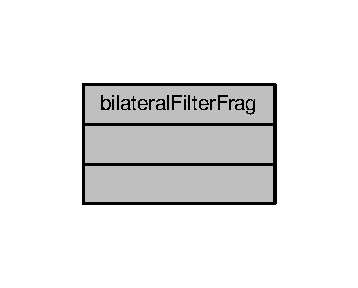
\includegraphics[width=172pt]{classbilateral_filter_frag__coll__graph}
\end{center}
\end{figure}


\subsection{Detailed Description}
Fragment shader to apply bilateral filter blur on an input. 

The documentation for this class was generated from the following file\-:\begin{DoxyCompactItemize}
\item 
shaders/\hyperlink{bilateral_filter_frag_8glsl}{bilateral\-Filter\-Frag.\-glsl}\end{DoxyCompactItemize}

\hypertarget{classbilateral_filter_vert}{\section{bilateral\-Filter\-Vert Class Reference}
\label{classbilateral_filter_vert}\index{bilateral\-Filter\-Vert@{bilateral\-Filter\-Vert}}
}


Vertex shader for our bilateral filter shader. Just passes through positions and tex coords.  




\subsection{Detailed Description}
Vertex shader for our bilateral filter shader. Just passes through positions and tex coords. 

The documentation for this class was generated from the following file\-:\begin{DoxyCompactItemize}
\item 
shaders/\hyperlink{bilateral_filter_vert_8glsl}{bilateral\-Filter\-Vert.\-glsl}\end{DoxyCompactItemize}

\hypertarget{classfluid_shader_frag}{\section{fluid\-Shader\-Frag Class Reference}
\label{classfluid_shader_frag}\index{fluid\-Shader\-Frag@{fluid\-Shader\-Frag}}
}


Fragment shader to apply the final shading of our fluid. This calculates the fragment normals.  




Collaboration diagram for fluid\-Shader\-Frag\-:\nopagebreak
\begin{figure}[H]
\begin{center}
\leavevmode
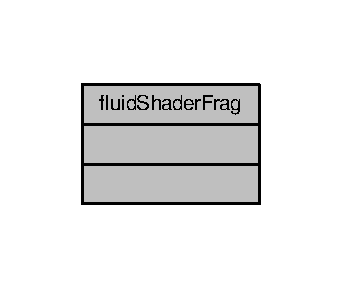
\includegraphics[width=164pt]{classfluid_shader_frag__coll__graph}
\end{center}
\end{figure}


\subsection{Detailed Description}
Fragment shader to apply the final shading of our fluid. This calculates the fragment normals. 

based on a depth pass texture. It also adds reflection and refraction based on a cube map. 

The documentation for this class was generated from the following file\-:\begin{DoxyCompactItemize}
\item 
shaders/\hyperlink{fluid_shader_frag_8glsl}{fluid\-Shader\-Frag.\-glsl}\end{DoxyCompactItemize}

\hypertarget{classfluid_shader_vert}{\section{fluid\-Shader\-Vert Class Reference}
\label{classfluid_shader_vert}\index{fluid\-Shader\-Vert@{fluid\-Shader\-Vert}}
}


Vertex shader for our fluid shader. Just passes through positions and tex coords.  




Collaboration diagram for fluid\-Shader\-Vert\-:\nopagebreak
\begin{figure}[H]
\begin{center}
\leavevmode
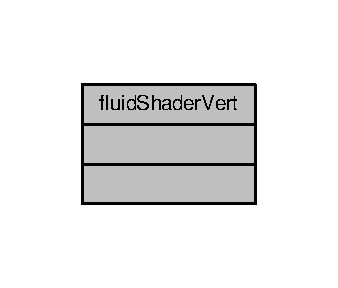
\includegraphics[width=162pt]{classfluid_shader_vert__coll__graph}
\end{center}
\end{figure}


\subsection{Detailed Description}
Vertex shader for our fluid shader. Just passes through positions and tex coords. 

The documentation for this class was generated from the following file\-:\begin{DoxyCompactItemize}
\item 
/home/dexternation/\-A\-G\-S\-D\-T\-Fluid\-Sim/shaders/\hyperlink{fluid_shader_vert_8glsl}{fluid\-Shader\-Vert.\-glsl}\end{DoxyCompactItemize}

\hypertarget{structlight_info}{\section{light\-Info Struct Reference}
\label{structlight_info}\index{light\-Info@{light\-Info}}
}


a structure to hold our light information  




Collaboration diagram for light\-Info\-:\nopagebreak
\begin{figure}[H]
\begin{center}
\leavevmode
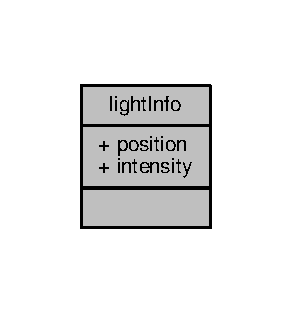
\includegraphics[width=140pt]{structlight_info__coll__graph}
\end{center}
\end{figure}
\subsection*{Public Attributes}
\begin{DoxyCompactItemize}
\item 
\hypertarget{structlight_info_a91464db499bb017224ed4137db3ad357}{vec4 {\bfseries position}}\label{structlight_info_a91464db499bb017224ed4137db3ad357}

\item 
\hypertarget{structlight_info_a0a3a282dd8998aed665222fd1902611f}{vec3 {\bfseries intensity}}\label{structlight_info_a0a3a282dd8998aed665222fd1902611f}

\end{DoxyCompactItemize}


\subsection{Detailed Description}
a structure to hold our light information 

The documentation for this struct was generated from the following file\-:\begin{DoxyCompactItemize}
\item 
/home/dexternation/\-A\-G\-S\-D\-T\-Fluid\-Sim/shaders/\hyperlink{fluid_shader_frag_8glsl}{fluid\-Shader\-Frag.\-glsl}\end{DoxyCompactItemize}

\hypertarget{class_main_window}{\section{Main\-Window Class Reference}
\label{class_main_window}\index{Main\-Window@{Main\-Window}}
}


Inheritance diagram for Main\-Window\-:\nopagebreak
\begin{figure}[H]
\begin{center}
\leavevmode
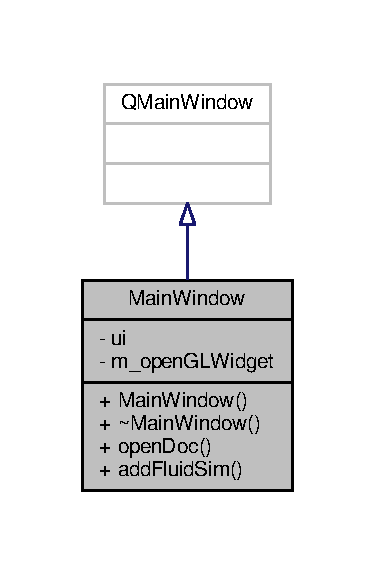
\includegraphics[width=180pt]{class_main_window__inherit__graph}
\end{center}
\end{figure}


Collaboration diagram for Main\-Window\-:\nopagebreak
\begin{figure}[H]
\begin{center}
\leavevmode
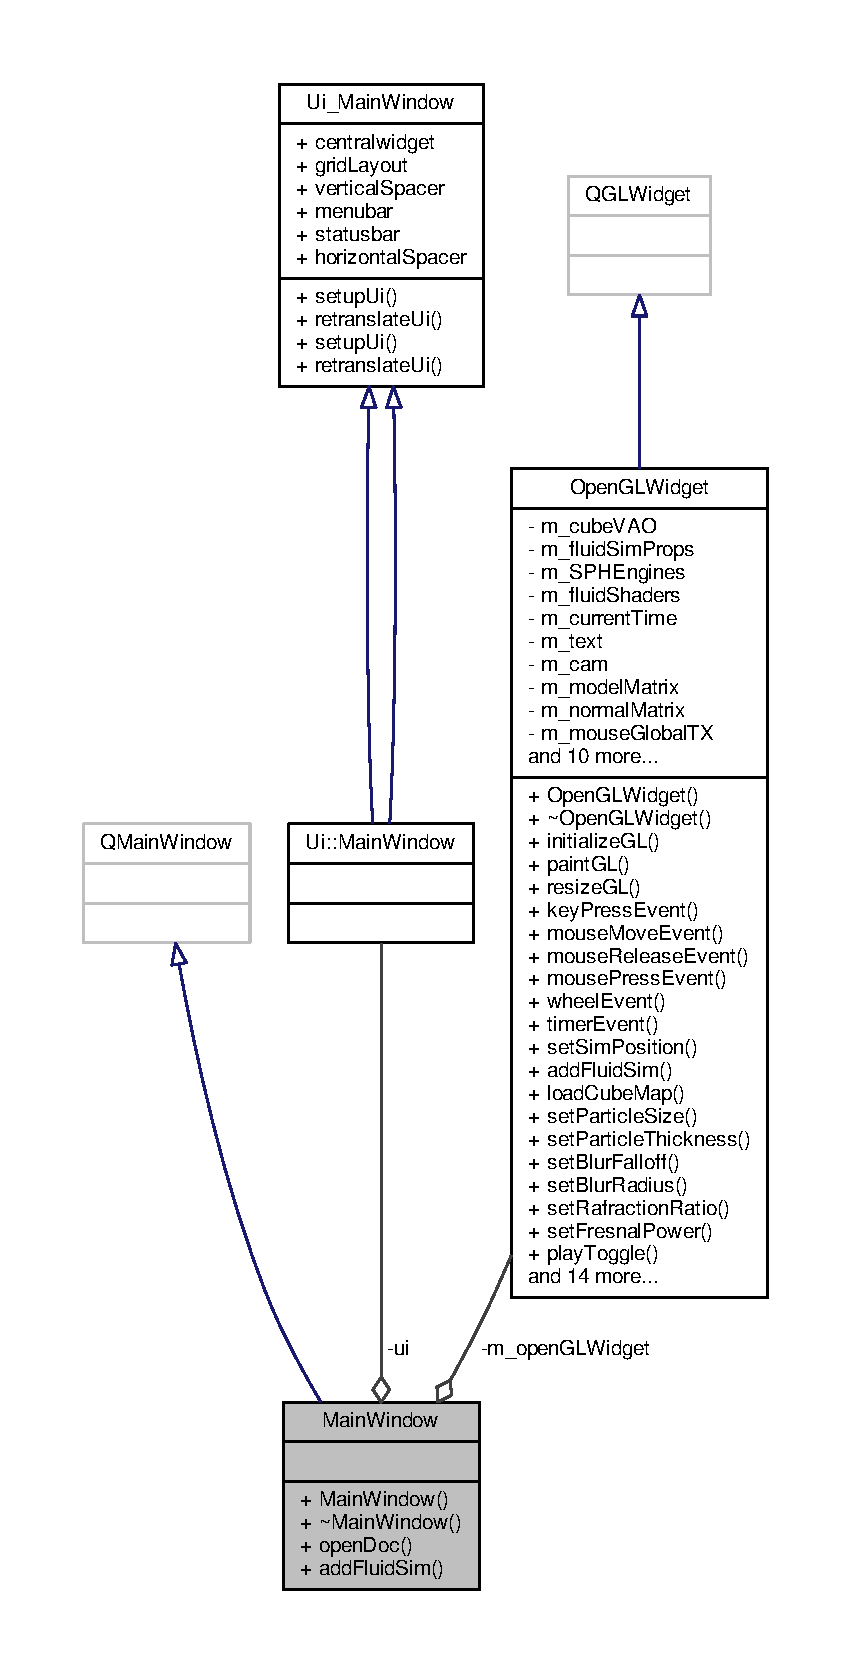
\includegraphics[height=550pt]{class_main_window__coll__graph}
\end{center}
\end{figure}
\subsection*{Public Slots}
\begin{DoxyCompactItemize}
\item 
\hypertarget{class_main_window_a452fc3db76653e3355cd9eb81bc4f0cf}{void \hyperlink{class_main_window_a452fc3db76653e3355cd9eb81bc4f0cf}{open\-Doc} ()}\label{class_main_window_a452fc3db76653e3355cd9eb81bc4f0cf}

\begin{DoxyCompactList}\small\item\em open documentation slot \end{DoxyCompactList}\item 
\hypertarget{class_main_window_ab411c296f30fa6a6f7dffe17826dd85f}{void \hyperlink{class_main_window_ab411c296f30fa6a6f7dffe17826dd85f}{add\-Fluid\-Sim} ()}\label{class_main_window_ab411c296f30fa6a6f7dffe17826dd85f}

\begin{DoxyCompactList}\small\item\em adds a fluid sim to our opengl scene \end{DoxyCompactList}\end{DoxyCompactItemize}
\subsection*{Public Member Functions}
\begin{DoxyCompactItemize}
\item 
\hypertarget{class_main_window_a8b244be8b7b7db1b08de2a2acb9409db}{{\bfseries Main\-Window} (Q\-Widget $\ast$parent=0)}\label{class_main_window_a8b244be8b7b7db1b08de2a2acb9409db}

\end{DoxyCompactItemize}
\subsection*{Private Attributes}
\begin{DoxyCompactItemize}
\item 
\hypertarget{class_main_window_a35466a70ed47252a0191168126a352a5}{\hyperlink{class_ui_1_1_main_window}{Ui\-::\-Main\-Window} $\ast$ {\bfseries ui}}\label{class_main_window_a35466a70ed47252a0191168126a352a5}

\item 
\hypertarget{class_main_window_af310504f60344259d8a43e495e90e54d}{\hyperlink{class_open_g_l_widget}{Open\-G\-L\-Widget} $\ast$ {\bfseries m\-\_\-open\-G\-L\-Widget}}\label{class_main_window_af310504f60344259d8a43e495e90e54d}

\end{DoxyCompactItemize}


The documentation for this class was generated from the following files\-:\begin{DoxyCompactItemize}
\item 
/home/dexternation/\-A\-G\-S\-D\-T\-Fluid\-Sim/include/mainwindow.\-h\item 
/home/dexternation/\-A\-G\-S\-D\-T\-Fluid\-Sim/src/mainwindow.\-cpp\end{DoxyCompactItemize}

\hypertarget{class_ui_1_1_main_window}{\section{Ui\-:\-:Main\-Window Class Reference}
\label{class_ui_1_1_main_window}\index{Ui\-::\-Main\-Window@{Ui\-::\-Main\-Window}}
}
Inheritance diagram for Ui\-:\-:Main\-Window\-:\begin{figure}[H]
\begin{center}
\leavevmode
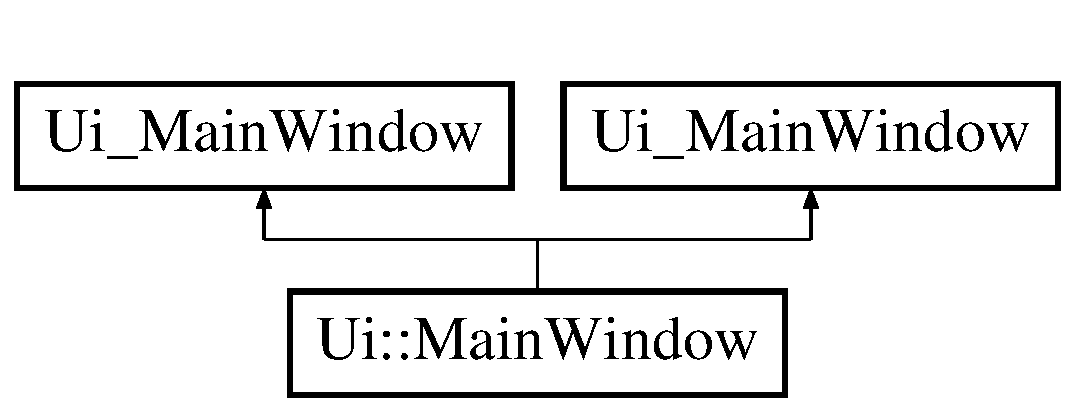
\includegraphics[height=2.000000cm]{class_ui_1_1_main_window}
\end{center}
\end{figure}
\subsection*{Additional Inherited Members}


The documentation for this class was generated from the following file\-:\begin{DoxyCompactItemize}
\item 
include/ui\-\_\-mainwindow.\-h\end{DoxyCompactItemize}

\hypertarget{class_open_g_l_widget}{\section{Open\-G\-L\-Widget Class Reference}
\label{class_open_g_l_widget}\index{Open\-G\-L\-Widget@{Open\-G\-L\-Widget}}
}


Basic Qt widget that holds a Open\-G\-L context.  




{\ttfamily \#include $<$Open\-G\-L\-Widget.\-h$>$}

Inheritance diagram for Open\-G\-L\-Widget\-:\begin{figure}[H]
\begin{center}
\leavevmode
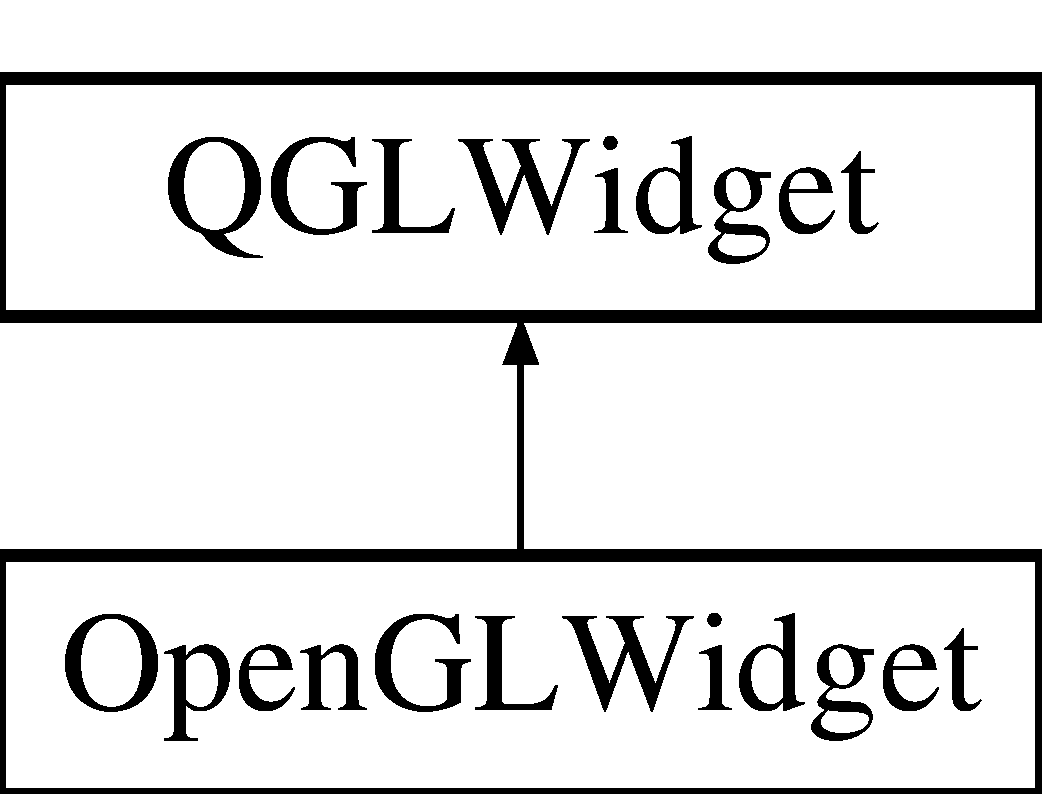
\includegraphics[height=2.000000cm]{class_open_g_l_widget}
\end{center}
\end{figure}
\subsection*{Public Slots}
\begin{DoxyCompactItemize}
\item 
void \hyperlink{class_open_g_l_widget_a6bc6106c82580697f386fdfd2fdb3a12}{set\-Sim\-Position} (float \-\_\-x, float \-\_\-y, float \-\_\-z, int \-\_\-sim\-No=0)
\begin{DoxyCompactList}\small\item\em slot to set sim position \end{DoxyCompactList}\item 
\hypertarget{class_open_g_l_widget_a9ccb72da15f23a16fb74b270a9e19489}{void \hyperlink{class_open_g_l_widget_a9ccb72da15f23a16fb74b270a9e19489}{add\-Fluid\-Sim} ()}\label{class_open_g_l_widget_a9ccb72da15f23a16fb74b270a9e19489}

\begin{DoxyCompactList}\small\item\em slot to add a fluid simulation to our scene \end{DoxyCompactList}\item 
void \hyperlink{class_open_g_l_widget_a39018f8fc74ce591bfac884c277621e6}{load\-Cube\-Map} (Q\-String \-\_\-loc)
\begin{DoxyCompactList}\small\item\em slot to load cube maps to for our enironment map \end{DoxyCompactList}\item 
void \hyperlink{class_open_g_l_widget_a3cdaf60ea4f98ee4782dec21b4810a41}{set\-Particle\-Size} (float \-\_\-size, int \-\_\-sim\-No=0)
\begin{DoxyCompactList}\small\item\em a slot to change our particle size \end{DoxyCompactList}\item 
void \hyperlink{class_open_g_l_widget_aec967838bdff11519892bc05a5d930b0}{set\-Particle\-Thickness} (float \-\_\-thickness, int \-\_\-sim\-No=0)
\begin{DoxyCompactList}\small\item\em a slot to change our particle thickess \end{DoxyCompactList}\item 
void \hyperlink{class_open_g_l_widget_a8e96b44ed40ec8a5fe726f427f01e6fe}{set\-Blur\-Falloff} (float \-\_\-falloff, int \-\_\-sim\-No=0)
\begin{DoxyCompactList}\small\item\em a slot to change our bilateral filter blur falloff \end{DoxyCompactList}\item 
void \hyperlink{class_open_g_l_widget_add467ba5217218564d08ffb638b2f190}{set\-Blur\-Radius} (float \-\_\-radius, int \-\_\-sim\-No=0)
\begin{DoxyCompactList}\small\item\em a slot to change our bilateral filter blur radius \end{DoxyCompactList}\item 
void \hyperlink{class_open_g_l_widget_a9ad49f35e3a76ec5ea58cedbe73afa34}{set\-Rafraction\-Ratio} (float \-\_\-eta, int \-\_\-sim\-No=0)
\begin{DoxyCompactList}\small\item\em a slot to set the refraction ratio of our fluid \end{DoxyCompactList}\item 
void \hyperlink{class_open_g_l_widget_adc34d0b2bed5d7a7f2d5b92fa1b82889}{set\-Fresnal\-Power} (float \-\_\-power, int \-\_\-sim\-No=0)
\begin{DoxyCompactList}\small\item\em a slot to set the fresnal power of our fluid \end{DoxyCompactList}\item 
void \hyperlink{class_open_g_l_widget_a2d1d9bb18d20f1479cb86e832ab17fd2}{play\-Toggle} (int \-\_\-sim\-No=0)
\begin{DoxyCompactList}\small\item\em play/pause toggle slot \end{DoxyCompactList}\item 
void \hyperlink{class_open_g_l_widget_a84585fd40a1fad03bbd118436f5fc477}{set\-Mass} (float \-\_\-mass, int \-\_\-sim\-No=0)
\begin{DoxyCompactList}\small\item\em set volume of our fluid slot \end{DoxyCompactList}\item 
void \hyperlink{class_open_g_l_widget_a785cd8493ea4c1a24a19a16835de4577}{set\-Density} (float \-\_\-den, int \-\_\-sim\-No=0)
\begin{DoxyCompactList}\small\item\em set density of our fluid slot \end{DoxyCompactList}\item 
void \hyperlink{class_open_g_l_widget_aad4c9ceaedc57507d3e9504d15dd8f4a}{set\-Visc\-Coef} (float \-\_\-visc, int \-\_\-sim\-No=0)
\begin{DoxyCompactList}\small\item\em set viscoty coeficient of our fluid slot \end{DoxyCompactList}\item 
void \hyperlink{class_open_g_l_widget_a806e81697e0c6bf0992696ab948bc1c5}{set\-Gas\-Const} (double \-\_\-gas\-Const, int \-\_\-sim\-No=0)
\begin{DoxyCompactList}\small\item\em set gas constant of our fluid slot \end{DoxyCompactList}\item 
void \hyperlink{class_open_g_l_widget_af0f0474b4ff16318e6cf2e7479b369c7}{set\-Smoothing\-Length} (float \-\_\-len, int \-\_\-sim\-No=0)
\begin{DoxyCompactList}\small\item\em set smoothing length of our fluid slot \end{DoxyCompactList}\item 
void \hyperlink{class_open_g_l_widget_a559ba717c412258c234ce5865c0b6976}{set\-Fluid\-Color} (Q\-Color \-\_\-col, int \-\_\-sim\-No=0)
\begin{DoxyCompactList}\small\item\em set the color of our fluid slot \end{DoxyCompactList}\item 
void \hyperlink{class_open_g_l_widget_a3c415ea6ecc1ccf6df49b08df74bbd1a}{set\-Playback\-Speed} (float \-\_\-speed, int \-\_\-sim\-No=0)
\begin{DoxyCompactList}\small\item\em a slot to set the playback speed of our simulation \end{DoxyCompactList}\item 
void \hyperlink{class_open_g_l_widget_ac8a71d325740372032c0061d3bf1daa0}{set\-Sim\-Time\-Step} (float \-\_\-time\-Step, int \-\_\-sim\-No=0)
\begin{DoxyCompactList}\small\item\em a slot to set the time step of our simulation \end{DoxyCompactList}\item 
void \hyperlink{class_open_g_l_widget_acc54210918549bd628db0080d576b483}{reset\-Sim} (int \-\_\-sim\-No)
\begin{DoxyCompactList}\small\item\em a slot to reset our simulation and remove all particles \end{DoxyCompactList}\item 
void \hyperlink{class_open_g_l_widget_ac4d67ea702f268f7d072e94a569cb5f0}{set\-Spawn\-Box\-Position} (float \-\_\-x, float \-\_\-y, float \-\_\-z, int \-\_\-sim\-No=0)
\begin{DoxyCompactList}\small\item\em a slot to set the spawn box position in our simulation \end{DoxyCompactList}\item 
void \hyperlink{class_open_g_l_widget_a60e5e6f2845384c3faeaa11c0fb800b4}{set\-Spawn\-Box\-Size} (float \-\_\-size, int \-\_\-sim\-No=0)
\begin{DoxyCompactList}\small\item\em a slot to set the spawn box size in our simulation \end{DoxyCompactList}\item 
void \hyperlink{class_open_g_l_widget_adce23eb4fa8b5a1d1ac0403c911abb37}{add\-Particles\-To\-Sim} (int \-\_\-num\-Particles, int \-\_\-sim\-No=0)
\begin{DoxyCompactList}\small\item\em slot to add particles to our simulation \end{DoxyCompactList}\item 
void \hyperlink{class_open_g_l_widget_a9ca3397753dcfbc56ada94d1e91000ed}{set\-Vel\-Correction} (float \-\_\-val, int \-\_\-sim\-No=0)
\begin{DoxyCompactList}\small\item\em slot to set the velocity correction of our simulation \end{DoxyCompactList}\item 
void \hyperlink{class_open_g_l_widget_ac4dea29c4b53c1c4906dacd4aa35d975}{set\-Display\-Hud} (bool \-\_\-display, int \-\_\-sim\-No=0)
\begin{DoxyCompactList}\small\item\em slot to toggle display of the hud of our simulatio \end{DoxyCompactList}\end{DoxyCompactItemize}
\subsection*{Public Member Functions}
\begin{DoxyCompactItemize}
\item 
\hyperlink{class_open_g_l_widget_a60b9008fd7762190918d5e2528a57248}{Open\-G\-L\-Widget} (const Q\-G\-L\-Format \-\_\-format, Q\-Widget $\ast$\-\_\-parent=0)
\begin{DoxyCompactList}\small\item\em ctor for our N\-G\-L drawing class \end{DoxyCompactList}\item 
\hypertarget{class_open_g_l_widget_a293847f6a7e6c40344a1acfca3e9eb51}{\hyperlink{class_open_g_l_widget_a293847f6a7e6c40344a1acfca3e9eb51}{$\sim$\-Open\-G\-L\-Widget} ()}\label{class_open_g_l_widget_a293847f6a7e6c40344a1acfca3e9eb51}

\begin{DoxyCompactList}\small\item\em dtor must close down and release Open\-G\-L resources \end{DoxyCompactList}\item 
\hypertarget{class_open_g_l_widget_a570df546f7206455c57addb624906576}{void \hyperlink{class_open_g_l_widget_a570df546f7206455c57addb624906576}{initialize\-G\-L} ()}\label{class_open_g_l_widget_a570df546f7206455c57addb624906576}

\begin{DoxyCompactList}\small\item\em the virtual initialize class is called once when the window is created and we have a valid G\-L context use this to setup any default G\-L stuff \end{DoxyCompactList}\item 
\hypertarget{class_open_g_l_widget_a260a543726f601659cbd1809b90f9e4b}{void \hyperlink{class_open_g_l_widget_a260a543726f601659cbd1809b90f9e4b}{paint\-G\-L} ()}\label{class_open_g_l_widget_a260a543726f601659cbd1809b90f9e4b}

\begin{DoxyCompactList}\small\item\em this is called everytime we want to draw the scene \end{DoxyCompactList}\item 
\hypertarget{class_open_g_l_widget_a55cf4659a7f10207fb6ab3fcf9273abc}{void \hyperlink{class_open_g_l_widget_a55cf4659a7f10207fb6ab3fcf9273abc}{resize\-G\-L} (const int \-\_\-w, const int \-\_\-h)}\label{class_open_g_l_widget_a55cf4659a7f10207fb6ab3fcf9273abc}

\begin{DoxyCompactList}\small\item\em called to resize the window \end{DoxyCompactList}\item 
\hypertarget{class_open_g_l_widget_a2e7ec0372fb6b2a0eb85a9524cfdd7fd}{void \hyperlink{class_open_g_l_widget_a2e7ec0372fb6b2a0eb85a9524cfdd7fd}{key\-Press\-Event} (Q\-Key\-Event $\ast$\-\_\-event)}\label{class_open_g_l_widget_a2e7ec0372fb6b2a0eb85a9524cfdd7fd}

\begin{DoxyCompactList}\small\item\em keyboard press event \end{DoxyCompactList}\item 
\hypertarget{class_open_g_l_widget_aa6d543f552c813df3b3a78dc5c4899fd}{void \hyperlink{class_open_g_l_widget_aa6d543f552c813df3b3a78dc5c4899fd}{mouse\-Move\-Event} (Q\-Mouse\-Event $\ast$\-\_\-event)}\label{class_open_g_l_widget_aa6d543f552c813df3b3a78dc5c4899fd}

\begin{DoxyCompactList}\small\item\em mouse move \end{DoxyCompactList}\item 
\hypertarget{class_open_g_l_widget_aa3f5541e5da2d5c52ca16b99f40dfd75}{void \hyperlink{class_open_g_l_widget_aa3f5541e5da2d5c52ca16b99f40dfd75}{mouse\-Release\-Event} (Q\-Mouse\-Event $\ast$\-\_\-event)}\label{class_open_g_l_widget_aa3f5541e5da2d5c52ca16b99f40dfd75}

\begin{DoxyCompactList}\small\item\em mouse button release \end{DoxyCompactList}\item 
\hypertarget{class_open_g_l_widget_adaab83f0bed689b0765d42b6ae760220}{void \hyperlink{class_open_g_l_widget_adaab83f0bed689b0765d42b6ae760220}{mouse\-Press\-Event} (Q\-Mouse\-Event $\ast$\-\_\-event)}\label{class_open_g_l_widget_adaab83f0bed689b0765d42b6ae760220}

\begin{DoxyCompactList}\small\item\em mouse button press \end{DoxyCompactList}\item 
void \hyperlink{class_open_g_l_widget_a0682546d360b7ce9ae1dce31a090cfca}{wheel\-Event} (Q\-Wheel\-Event $\ast$\-\_\-event)
\begin{DoxyCompactList}\small\item\em this method is called everytime the mouse wheel is moved inherited from Q\-Object and overridden here. \end{DoxyCompactList}\item 
\hypertarget{class_open_g_l_widget_a11473cec64e843211458fd83f9d6ad72}{void \hyperlink{class_open_g_l_widget_a11473cec64e843211458fd83f9d6ad72}{timer\-Event} (Q\-Timer\-Event $\ast$)}\label{class_open_g_l_widget_a11473cec64e843211458fd83f9d6ad72}

\begin{DoxyCompactList}\small\item\em a timer event function from the Q\-\_\-object \end{DoxyCompactList}\end{DoxyCompactItemize}


\subsection{Detailed Description}
Basic Qt widget that holds a Open\-G\-L context. 

\begin{DoxyAuthor}{Author}
Declan Russell 
\end{DoxyAuthor}
\begin{DoxyVersion}{Version}
1.\-0 
\end{DoxyVersion}
\begin{DoxyDate}{Date}
2/3/15 Initial version 
\end{DoxyDate}


\subsection{Constructor \& Destructor Documentation}
\hypertarget{class_open_g_l_widget_a60b9008fd7762190918d5e2528a57248}{\index{Open\-G\-L\-Widget@{Open\-G\-L\-Widget}!Open\-G\-L\-Widget@{Open\-G\-L\-Widget}}
\index{Open\-G\-L\-Widget@{Open\-G\-L\-Widget}!OpenGLWidget@{Open\-G\-L\-Widget}}
\subsubsection[{Open\-G\-L\-Widget}]{\setlength{\rightskip}{0pt plus 5cm}Open\-G\-L\-Widget\-::\-Open\-G\-L\-Widget (
\begin{DoxyParamCaption}
\item[{const Q\-G\-L\-Format}]{\-\_\-format, }
\item[{Q\-Widget $\ast$}]{\-\_\-parent = {\ttfamily 0}}
\end{DoxyParamCaption}
)\hspace{0.3cm}{\ttfamily [explicit]}}}\label{class_open_g_l_widget_a60b9008fd7762190918d5e2528a57248}


ctor for our N\-G\-L drawing class 


\begin{DoxyParams}[1]{Parameters}
\mbox{\tt in}  & {\em parent} & the parent window to the class \\
\hline
\end{DoxyParams}


\subsection{Member Function Documentation}
\hypertarget{class_open_g_l_widget_adce23eb4fa8b5a1d1ac0403c911abb37}{\index{Open\-G\-L\-Widget@{Open\-G\-L\-Widget}!add\-Particles\-To\-Sim@{add\-Particles\-To\-Sim}}
\index{add\-Particles\-To\-Sim@{add\-Particles\-To\-Sim}!OpenGLWidget@{Open\-G\-L\-Widget}}
\subsubsection[{add\-Particles\-To\-Sim}]{\setlength{\rightskip}{0pt plus 5cm}void Open\-G\-L\-Widget\-::add\-Particles\-To\-Sim (
\begin{DoxyParamCaption}
\item[{int}]{\-\_\-num\-Particles, }
\item[{int}]{\-\_\-sim\-No = {\ttfamily 0}}
\end{DoxyParamCaption}
)\hspace{0.3cm}{\ttfamily [inline]}, {\ttfamily [slot]}}}\label{class_open_g_l_widget_adce23eb4fa8b5a1d1ac0403c911abb37}


slot to add particles to our simulation 


\begin{DoxyParams}{Parameters}
{\em \-\_\-num\-Particles} & -\/ number of particles to add to simulation \\
\hline
{\em \-\_\-sim\-No} & -\/ simulation to add particles to \\
\hline
\end{DoxyParams}
\hypertarget{class_open_g_l_widget_a39018f8fc74ce591bfac884c277621e6}{\index{Open\-G\-L\-Widget@{Open\-G\-L\-Widget}!load\-Cube\-Map@{load\-Cube\-Map}}
\index{load\-Cube\-Map@{load\-Cube\-Map}!OpenGLWidget@{Open\-G\-L\-Widget}}
\subsubsection[{load\-Cube\-Map}]{\setlength{\rightskip}{0pt plus 5cm}void Open\-G\-L\-Widget\-::load\-Cube\-Map (
\begin{DoxyParamCaption}
\item[{Q\-String}]{\-\_\-loc}
\end{DoxyParamCaption}
)\hspace{0.3cm}{\ttfamily [slot]}}}\label{class_open_g_l_widget_a39018f8fc74ce591bfac884c277621e6}


slot to load cube maps to for our enironment map 

this function pressumes that all our cube map textures are in one texture 
\begin{DoxyParams}{Parameters}
{\em \-\_\-loc} & -\/ the location of our cube map texture \\
\hline
\end{DoxyParams}
\hypertarget{class_open_g_l_widget_a2d1d9bb18d20f1479cb86e832ab17fd2}{\index{Open\-G\-L\-Widget@{Open\-G\-L\-Widget}!play\-Toggle@{play\-Toggle}}
\index{play\-Toggle@{play\-Toggle}!OpenGLWidget@{Open\-G\-L\-Widget}}
\subsubsection[{play\-Toggle}]{\setlength{\rightskip}{0pt plus 5cm}void Open\-G\-L\-Widget\-::play\-Toggle (
\begin{DoxyParamCaption}
\item[{int}]{\-\_\-sim\-No = {\ttfamily 0}}
\end{DoxyParamCaption}
)\hspace{0.3cm}{\ttfamily [inline]}, {\ttfamily [slot]}}}\label{class_open_g_l_widget_a2d1d9bb18d20f1479cb86e832ab17fd2}


play/pause toggle slot 


\begin{DoxyParams}{Parameters}
{\em \-\_\-sim\-No} & -\/ which simulation we want to toggle play \\
\hline
\end{DoxyParams}
\hypertarget{class_open_g_l_widget_acc54210918549bd628db0080d576b483}{\index{Open\-G\-L\-Widget@{Open\-G\-L\-Widget}!reset\-Sim@{reset\-Sim}}
\index{reset\-Sim@{reset\-Sim}!OpenGLWidget@{Open\-G\-L\-Widget}}
\subsubsection[{reset\-Sim}]{\setlength{\rightskip}{0pt plus 5cm}void Open\-G\-L\-Widget\-::reset\-Sim (
\begin{DoxyParamCaption}
\item[{int}]{\-\_\-sim\-No}
\end{DoxyParamCaption}
)\hspace{0.3cm}{\ttfamily [inline]}, {\ttfamily [slot]}}}\label{class_open_g_l_widget_acc54210918549bd628db0080d576b483}


a slot to reset our simulation and remove all particles 

\-\_\-sim\-No -\/ simulation number to reset \hypertarget{class_open_g_l_widget_a8e96b44ed40ec8a5fe726f427f01e6fe}{\index{Open\-G\-L\-Widget@{Open\-G\-L\-Widget}!set\-Blur\-Falloff@{set\-Blur\-Falloff}}
\index{set\-Blur\-Falloff@{set\-Blur\-Falloff}!OpenGLWidget@{Open\-G\-L\-Widget}}
\subsubsection[{set\-Blur\-Falloff}]{\setlength{\rightskip}{0pt plus 5cm}void Open\-G\-L\-Widget\-::set\-Blur\-Falloff (
\begin{DoxyParamCaption}
\item[{float}]{\-\_\-falloff, }
\item[{int}]{\-\_\-sim\-No = {\ttfamily 0}}
\end{DoxyParamCaption}
)\hspace{0.3cm}{\ttfamily [inline]}, {\ttfamily [slot]}}}\label{class_open_g_l_widget_a8e96b44ed40ec8a5fe726f427f01e6fe}


a slot to change our bilateral filter blur falloff 


\begin{DoxyParams}{Parameters}
{\em \-\_\-falloff} & -\/ bilateral blur falloff \\
\hline
{\em \-\_\-sim\-No} & -\/ which simulation we want to change the blur fall off in \\
\hline
\end{DoxyParams}
\hypertarget{class_open_g_l_widget_add467ba5217218564d08ffb638b2f190}{\index{Open\-G\-L\-Widget@{Open\-G\-L\-Widget}!set\-Blur\-Radius@{set\-Blur\-Radius}}
\index{set\-Blur\-Radius@{set\-Blur\-Radius}!OpenGLWidget@{Open\-G\-L\-Widget}}
\subsubsection[{set\-Blur\-Radius}]{\setlength{\rightskip}{0pt plus 5cm}void Open\-G\-L\-Widget\-::set\-Blur\-Radius (
\begin{DoxyParamCaption}
\item[{float}]{\-\_\-radius, }
\item[{int}]{\-\_\-sim\-No = {\ttfamily 0}}
\end{DoxyParamCaption}
)\hspace{0.3cm}{\ttfamily [inline]}, {\ttfamily [slot]}}}\label{class_open_g_l_widget_add467ba5217218564d08ffb638b2f190}


a slot to change our bilateral filter blur radius 


\begin{DoxyParams}{Parameters}
{\em \-\_\-radius} & -\/ bilateral blur radius \\
\hline
{\em \-\_\-sim\-No} & -\/ which simulation we want to change the blur radius in \\
\hline
\end{DoxyParams}
\hypertarget{class_open_g_l_widget_a785cd8493ea4c1a24a19a16835de4577}{\index{Open\-G\-L\-Widget@{Open\-G\-L\-Widget}!set\-Density@{set\-Density}}
\index{set\-Density@{set\-Density}!OpenGLWidget@{Open\-G\-L\-Widget}}
\subsubsection[{set\-Density}]{\setlength{\rightskip}{0pt plus 5cm}void Open\-G\-L\-Widget\-::set\-Density (
\begin{DoxyParamCaption}
\item[{float}]{\-\_\-den, }
\item[{int}]{\-\_\-sim\-No = {\ttfamily 0}}
\end{DoxyParamCaption}
)\hspace{0.3cm}{\ttfamily [inline]}, {\ttfamily [slot]}}}\label{class_open_g_l_widget_a785cd8493ea4c1a24a19a16835de4577}


set density of our fluid slot 


\begin{DoxyParams}{Parameters}
{\em \-\_\-den} & -\/ desired rest density \\
\hline
{\em \-\_\-sim\-No} & -\/ which simulation we want to change \\
\hline
\end{DoxyParams}
\hypertarget{class_open_g_l_widget_ac4dea29c4b53c1c4906dacd4aa35d975}{\index{Open\-G\-L\-Widget@{Open\-G\-L\-Widget}!set\-Display\-Hud@{set\-Display\-Hud}}
\index{set\-Display\-Hud@{set\-Display\-Hud}!OpenGLWidget@{Open\-G\-L\-Widget}}
\subsubsection[{set\-Display\-Hud}]{\setlength{\rightskip}{0pt plus 5cm}void Open\-G\-L\-Widget\-::set\-Display\-Hud (
\begin{DoxyParamCaption}
\item[{bool}]{\-\_\-display, }
\item[{int}]{\-\_\-sim\-No = {\ttfamily 0}}
\end{DoxyParamCaption}
)\hspace{0.3cm}{\ttfamily [inline]}, {\ttfamily [slot]}}}\label{class_open_g_l_widget_ac4dea29c4b53c1c4906dacd4aa35d975}


slot to toggle display of the hud of our simulatio 


\begin{DoxyParams}{Parameters}
{\em \-\_\-display} & -\/ bool to indicate if we want to display it or not \\
\hline
{\em \-\_\-sim\-No} & -\/ simulation we wish to display Hud \\
\hline
\end{DoxyParams}
\hypertarget{class_open_g_l_widget_a559ba717c412258c234ce5865c0b6976}{\index{Open\-G\-L\-Widget@{Open\-G\-L\-Widget}!set\-Fluid\-Color@{set\-Fluid\-Color}}
\index{set\-Fluid\-Color@{set\-Fluid\-Color}!OpenGLWidget@{Open\-G\-L\-Widget}}
\subsubsection[{set\-Fluid\-Color}]{\setlength{\rightskip}{0pt plus 5cm}void Open\-G\-L\-Widget\-::set\-Fluid\-Color (
\begin{DoxyParamCaption}
\item[{Q\-Color}]{\-\_\-col, }
\item[{int}]{\-\_\-sim\-No = {\ttfamily 0}}
\end{DoxyParamCaption}
)\hspace{0.3cm}{\ttfamily [inline]}, {\ttfamily [slot]}}}\label{class_open_g_l_widget_a559ba717c412258c234ce5865c0b6976}


set the color of our fluid slot 


\begin{DoxyParams}{Parameters}
{\em \-\_\-col} & -\/ desired color to set the fluid to \\
\hline
{\em \-\_\-sim\-No} & -\/ which simulation we want to change the color in \\
\hline
\end{DoxyParams}
\hypertarget{class_open_g_l_widget_adc34d0b2bed5d7a7f2d5b92fa1b82889}{\index{Open\-G\-L\-Widget@{Open\-G\-L\-Widget}!set\-Fresnal\-Power@{set\-Fresnal\-Power}}
\index{set\-Fresnal\-Power@{set\-Fresnal\-Power}!OpenGLWidget@{Open\-G\-L\-Widget}}
\subsubsection[{set\-Fresnal\-Power}]{\setlength{\rightskip}{0pt plus 5cm}void Open\-G\-L\-Widget\-::set\-Fresnal\-Power (
\begin{DoxyParamCaption}
\item[{float}]{\-\_\-power, }
\item[{int}]{\-\_\-sim\-No = {\ttfamily 0}}
\end{DoxyParamCaption}
)\hspace{0.3cm}{\ttfamily [inline]}, {\ttfamily [slot]}}}\label{class_open_g_l_widget_adc34d0b2bed5d7a7f2d5b92fa1b82889}


a slot to set the fresnal power of our fluid 


\begin{DoxyParams}{Parameters}
{\em \-\_\-power} & -\/ desired fresnal power of our fluid \\
\hline
{\em \-\_\-sim\-No} & -\/ which simulation we want to change the fresnal power in \\
\hline
\end{DoxyParams}
\hypertarget{class_open_g_l_widget_a806e81697e0c6bf0992696ab948bc1c5}{\index{Open\-G\-L\-Widget@{Open\-G\-L\-Widget}!set\-Gas\-Const@{set\-Gas\-Const}}
\index{set\-Gas\-Const@{set\-Gas\-Const}!OpenGLWidget@{Open\-G\-L\-Widget}}
\subsubsection[{set\-Gas\-Const}]{\setlength{\rightskip}{0pt plus 5cm}void Open\-G\-L\-Widget\-::set\-Gas\-Const (
\begin{DoxyParamCaption}
\item[{double}]{\-\_\-gas\-Const, }
\item[{int}]{\-\_\-sim\-No = {\ttfamily 0}}
\end{DoxyParamCaption}
)\hspace{0.3cm}{\ttfamily [inline]}, {\ttfamily [slot]}}}\label{class_open_g_l_widget_a806e81697e0c6bf0992696ab948bc1c5}


set gas constant of our fluid slot 


\begin{DoxyParams}{Parameters}
{\em \-\_\-gas\-Const} & -\/ gas constant \\
\hline
{\em \-\_\-sim\-No} & -\/ which simulation we want to change \\
\hline
\end{DoxyParams}
\hypertarget{class_open_g_l_widget_a84585fd40a1fad03bbd118436f5fc477}{\index{Open\-G\-L\-Widget@{Open\-G\-L\-Widget}!set\-Mass@{set\-Mass}}
\index{set\-Mass@{set\-Mass}!OpenGLWidget@{Open\-G\-L\-Widget}}
\subsubsection[{set\-Mass}]{\setlength{\rightskip}{0pt plus 5cm}void Open\-G\-L\-Widget\-::set\-Mass (
\begin{DoxyParamCaption}
\item[{float}]{\-\_\-mass, }
\item[{int}]{\-\_\-sim\-No = {\ttfamily 0}}
\end{DoxyParamCaption}
)\hspace{0.3cm}{\ttfamily [inline]}, {\ttfamily [slot]}}}\label{class_open_g_l_widget_a84585fd40a1fad03bbd118436f5fc477}


set volume of our fluid slot 


\begin{DoxyParams}{Parameters}
{\em \-\_\-mass} & -\/ desired mass of particles \\
\hline
{\em \-\_\-sim\-No} & -\/ which simulation we want to change \\
\hline
\end{DoxyParams}
\hypertarget{class_open_g_l_widget_a3cdaf60ea4f98ee4782dec21b4810a41}{\index{Open\-G\-L\-Widget@{Open\-G\-L\-Widget}!set\-Particle\-Size@{set\-Particle\-Size}}
\index{set\-Particle\-Size@{set\-Particle\-Size}!OpenGLWidget@{Open\-G\-L\-Widget}}
\subsubsection[{set\-Particle\-Size}]{\setlength{\rightskip}{0pt plus 5cm}void Open\-G\-L\-Widget\-::set\-Particle\-Size (
\begin{DoxyParamCaption}
\item[{float}]{\-\_\-size, }
\item[{int}]{\-\_\-sim\-No = {\ttfamily 0}}
\end{DoxyParamCaption}
)\hspace{0.3cm}{\ttfamily [inline]}, {\ttfamily [slot]}}}\label{class_open_g_l_widget_a3cdaf60ea4f98ee4782dec21b4810a41}


a slot to change our particle size 


\begin{DoxyParams}{Parameters}
{\em \-\_\-size} & -\/ particle size \\
\hline
{\em \-\_\-sim\-No} & -\/ which simulation we want to change the particle size in \\
\hline
\end{DoxyParams}
\hypertarget{class_open_g_l_widget_aec967838bdff11519892bc05a5d930b0}{\index{Open\-G\-L\-Widget@{Open\-G\-L\-Widget}!set\-Particle\-Thickness@{set\-Particle\-Thickness}}
\index{set\-Particle\-Thickness@{set\-Particle\-Thickness}!OpenGLWidget@{Open\-G\-L\-Widget}}
\subsubsection[{set\-Particle\-Thickness}]{\setlength{\rightskip}{0pt plus 5cm}void Open\-G\-L\-Widget\-::set\-Particle\-Thickness (
\begin{DoxyParamCaption}
\item[{float}]{\-\_\-thickness, }
\item[{int}]{\-\_\-sim\-No = {\ttfamily 0}}
\end{DoxyParamCaption}
)\hspace{0.3cm}{\ttfamily [inline]}, {\ttfamily [slot]}}}\label{class_open_g_l_widget_aec967838bdff11519892bc05a5d930b0}


a slot to change our particle thickess 


\begin{DoxyParams}{Parameters}
{\em \-\_\-thickness} & -\/ particle thickness \\
\hline
{\em \-\_\-sim\-No} & -\/ which simulation we want to change the thickness in \\
\hline
\end{DoxyParams}
\hypertarget{class_open_g_l_widget_a3c415ea6ecc1ccf6df49b08df74bbd1a}{\index{Open\-G\-L\-Widget@{Open\-G\-L\-Widget}!set\-Playback\-Speed@{set\-Playback\-Speed}}
\index{set\-Playback\-Speed@{set\-Playback\-Speed}!OpenGLWidget@{Open\-G\-L\-Widget}}
\subsubsection[{set\-Playback\-Speed}]{\setlength{\rightskip}{0pt plus 5cm}void Open\-G\-L\-Widget\-::set\-Playback\-Speed (
\begin{DoxyParamCaption}
\item[{float}]{\-\_\-speed, }
\item[{int}]{\-\_\-sim\-No = {\ttfamily 0}}
\end{DoxyParamCaption}
)\hspace{0.3cm}{\ttfamily [inline]}, {\ttfamily [slot]}}}\label{class_open_g_l_widget_a3c415ea6ecc1ccf6df49b08df74bbd1a}


a slot to set the playback speed of our simulation 


\begin{DoxyParams}{Parameters}
{\em \-\_\-speed} & -\/ the speed of play back as a percentage 100.\-f is real time \\
\hline
{\em \-\_\-sim\-No} & -\/ which simulation we want to change the play back speed in \\
\hline
\end{DoxyParams}
\hypertarget{class_open_g_l_widget_a9ad49f35e3a76ec5ea58cedbe73afa34}{\index{Open\-G\-L\-Widget@{Open\-G\-L\-Widget}!set\-Rafraction\-Ratio@{set\-Rafraction\-Ratio}}
\index{set\-Rafraction\-Ratio@{set\-Rafraction\-Ratio}!OpenGLWidget@{Open\-G\-L\-Widget}}
\subsubsection[{set\-Rafraction\-Ratio}]{\setlength{\rightskip}{0pt plus 5cm}void Open\-G\-L\-Widget\-::set\-Rafraction\-Ratio (
\begin{DoxyParamCaption}
\item[{float}]{\-\_\-eta, }
\item[{int}]{\-\_\-sim\-No = {\ttfamily 0}}
\end{DoxyParamCaption}
)\hspace{0.3cm}{\ttfamily [inline]}, {\ttfamily [slot]}}}\label{class_open_g_l_widget_a9ad49f35e3a76ec5ea58cedbe73afa34}


a slot to set the refraction ratio of our fluid 


\begin{DoxyParams}{Parameters}
{\em \-\_\-eta} & -\/ desired refraction ratio \\
\hline
{\em \-\_\-sim\-No} & -\/ which simulation we want to change the rafraction ratio in \\
\hline
\end{DoxyParams}
\hypertarget{class_open_g_l_widget_a6bc6106c82580697f386fdfd2fdb3a12}{\index{Open\-G\-L\-Widget@{Open\-G\-L\-Widget}!set\-Sim\-Position@{set\-Sim\-Position}}
\index{set\-Sim\-Position@{set\-Sim\-Position}!OpenGLWidget@{Open\-G\-L\-Widget}}
\subsubsection[{set\-Sim\-Position}]{\setlength{\rightskip}{0pt plus 5cm}void Open\-G\-L\-Widget\-::set\-Sim\-Position (
\begin{DoxyParamCaption}
\item[{float}]{\-\_\-x, }
\item[{float}]{\-\_\-y, }
\item[{float}]{\-\_\-z, }
\item[{int}]{\-\_\-sim\-No = {\ttfamily 0}}
\end{DoxyParamCaption}
)\hspace{0.3cm}{\ttfamily [inline]}, {\ttfamily [slot]}}}\label{class_open_g_l_widget_a6bc6106c82580697f386fdfd2fdb3a12}


slot to set sim position 


\begin{DoxyParams}{Parameters}
{\em \-\_\-x} & -\/ x position of our simulation \\
\hline
{\em \-\_\-y} & -\/ y position of our simulation \\
\hline
{\em \-\_\-z} & -\/ z position of our simualtion \\
\hline
{\em \-\_\-sim\-No} & -\/ simulation to set the position of \\
\hline
\end{DoxyParams}
\hypertarget{class_open_g_l_widget_ac8a71d325740372032c0061d3bf1daa0}{\index{Open\-G\-L\-Widget@{Open\-G\-L\-Widget}!set\-Sim\-Time\-Step@{set\-Sim\-Time\-Step}}
\index{set\-Sim\-Time\-Step@{set\-Sim\-Time\-Step}!OpenGLWidget@{Open\-G\-L\-Widget}}
\subsubsection[{set\-Sim\-Time\-Step}]{\setlength{\rightskip}{0pt plus 5cm}void Open\-G\-L\-Widget\-::set\-Sim\-Time\-Step (
\begin{DoxyParamCaption}
\item[{float}]{\-\_\-time\-Step, }
\item[{int}]{\-\_\-sim\-No = {\ttfamily 0}}
\end{DoxyParamCaption}
)\hspace{0.3cm}{\ttfamily [inline]}, {\ttfamily [slot]}}}\label{class_open_g_l_widget_ac8a71d325740372032c0061d3bf1daa0}


a slot to set the time step of our simulation 


\begin{DoxyParams}{Parameters}
{\em \-\_\-time\-Step} & -\/ the time\-Step of our simulation \\
\hline
{\em \-\_\-sim\-No} & -\/ which simulation we want to change the play back speed in \\
\hline
\end{DoxyParams}
\hypertarget{class_open_g_l_widget_af0f0474b4ff16318e6cf2e7479b369c7}{\index{Open\-G\-L\-Widget@{Open\-G\-L\-Widget}!set\-Smoothing\-Length@{set\-Smoothing\-Length}}
\index{set\-Smoothing\-Length@{set\-Smoothing\-Length}!OpenGLWidget@{Open\-G\-L\-Widget}}
\subsubsection[{set\-Smoothing\-Length}]{\setlength{\rightskip}{0pt plus 5cm}void Open\-G\-L\-Widget\-::set\-Smoothing\-Length (
\begin{DoxyParamCaption}
\item[{float}]{\-\_\-len, }
\item[{int}]{\-\_\-sim\-No = {\ttfamily 0}}
\end{DoxyParamCaption}
)\hspace{0.3cm}{\ttfamily [inline]}, {\ttfamily [slot]}}}\label{class_open_g_l_widget_af0f0474b4ff16318e6cf2e7479b369c7}


set smoothing length of our fluid slot 


\begin{DoxyParams}{Parameters}
{\em \-\_\-len} & -\/ smoothing length \\
\hline
{\em \-\_\-sim\-No} & -\/ which simulation we want to change our smoothing length in \\
\hline
\end{DoxyParams}
\hypertarget{class_open_g_l_widget_ac4d67ea702f268f7d072e94a569cb5f0}{\index{Open\-G\-L\-Widget@{Open\-G\-L\-Widget}!set\-Spawn\-Box\-Position@{set\-Spawn\-Box\-Position}}
\index{set\-Spawn\-Box\-Position@{set\-Spawn\-Box\-Position}!OpenGLWidget@{Open\-G\-L\-Widget}}
\subsubsection[{set\-Spawn\-Box\-Position}]{\setlength{\rightskip}{0pt plus 5cm}void Open\-G\-L\-Widget\-::set\-Spawn\-Box\-Position (
\begin{DoxyParamCaption}
\item[{float}]{\-\_\-x, }
\item[{float}]{\-\_\-y, }
\item[{float}]{\-\_\-z, }
\item[{int}]{\-\_\-sim\-No = {\ttfamily 0}}
\end{DoxyParamCaption}
)\hspace{0.3cm}{\ttfamily [inline]}, {\ttfamily [slot]}}}\label{class_open_g_l_widget_ac4d67ea702f268f7d072e94a569cb5f0}


a slot to set the spawn box position in our simulation 


\begin{DoxyParams}{Parameters}
{\em \-\_\-x} & -\/ x position of spawn box location \\
\hline
{\em \-\_\-y} & -\/ y position of spawn box location \\
\hline
{\em \-\_\-z} & -\/ z position of spawn box location \\
\hline
{\em \-\_\-sim\-No} & -\/ simulation number to set the spawn box location \\
\hline
\end{DoxyParams}
\hypertarget{class_open_g_l_widget_a60e5e6f2845384c3faeaa11c0fb800b4}{\index{Open\-G\-L\-Widget@{Open\-G\-L\-Widget}!set\-Spawn\-Box\-Size@{set\-Spawn\-Box\-Size}}
\index{set\-Spawn\-Box\-Size@{set\-Spawn\-Box\-Size}!OpenGLWidget@{Open\-G\-L\-Widget}}
\subsubsection[{set\-Spawn\-Box\-Size}]{\setlength{\rightskip}{0pt plus 5cm}void Open\-G\-L\-Widget\-::set\-Spawn\-Box\-Size (
\begin{DoxyParamCaption}
\item[{float}]{\-\_\-size, }
\item[{int}]{\-\_\-sim\-No = {\ttfamily 0}}
\end{DoxyParamCaption}
)\hspace{0.3cm}{\ttfamily [inline]}, {\ttfamily [slot]}}}\label{class_open_g_l_widget_a60e5e6f2845384c3faeaa11c0fb800b4}


a slot to set the spawn box size in our simulation 


\begin{DoxyParams}{Parameters}
{\em \-\_\-size} & -\/ desired spawn box size \\
\hline
{\em \-\_\-sim\-No} & -\/ simulation number to set the spawn box size \\
\hline
\end{DoxyParams}
\hypertarget{class_open_g_l_widget_a9ca3397753dcfbc56ada94d1e91000ed}{\index{Open\-G\-L\-Widget@{Open\-G\-L\-Widget}!set\-Vel\-Correction@{set\-Vel\-Correction}}
\index{set\-Vel\-Correction@{set\-Vel\-Correction}!OpenGLWidget@{Open\-G\-L\-Widget}}
\subsubsection[{set\-Vel\-Correction}]{\setlength{\rightskip}{0pt plus 5cm}void Open\-G\-L\-Widget\-::set\-Vel\-Correction (
\begin{DoxyParamCaption}
\item[{float}]{\-\_\-val, }
\item[{int}]{\-\_\-sim\-No = {\ttfamily 0}}
\end{DoxyParamCaption}
)\hspace{0.3cm}{\ttfamily [inline]}, {\ttfamily [slot]}}}\label{class_open_g_l_widget_a9ca3397753dcfbc56ada94d1e91000ed}


slot to set the velocity correction of our simulation 


\begin{DoxyParams}{Parameters}
{\em \-\_\-val} & -\/ value of velocity correction \\
\hline
{\em \-\_\-sim\-No} & -\/ simulation to set velocity correction in \\
\hline
\end{DoxyParams}
\hypertarget{class_open_g_l_widget_aad4c9ceaedc57507d3e9504d15dd8f4a}{\index{Open\-G\-L\-Widget@{Open\-G\-L\-Widget}!set\-Visc\-Coef@{set\-Visc\-Coef}}
\index{set\-Visc\-Coef@{set\-Visc\-Coef}!OpenGLWidget@{Open\-G\-L\-Widget}}
\subsubsection[{set\-Visc\-Coef}]{\setlength{\rightskip}{0pt plus 5cm}void Open\-G\-L\-Widget\-::set\-Visc\-Coef (
\begin{DoxyParamCaption}
\item[{float}]{\-\_\-visc, }
\item[{int}]{\-\_\-sim\-No = {\ttfamily 0}}
\end{DoxyParamCaption}
)\hspace{0.3cm}{\ttfamily [inline]}, {\ttfamily [slot]}}}\label{class_open_g_l_widget_aad4c9ceaedc57507d3e9504d15dd8f4a}


set viscoty coeficient of our fluid slot 


\begin{DoxyParams}{Parameters}
{\em \-\_\-visc} & -\/ viscosity coeficient \\
\hline
{\em \-\_\-sim\-No} & -\/ which simulation we want to change \\
\hline
\end{DoxyParams}
\hypertarget{class_open_g_l_widget_a0682546d360b7ce9ae1dce31a090cfca}{\index{Open\-G\-L\-Widget@{Open\-G\-L\-Widget}!wheel\-Event@{wheel\-Event}}
\index{wheel\-Event@{wheel\-Event}!OpenGLWidget@{Open\-G\-L\-Widget}}
\subsubsection[{wheel\-Event}]{\setlength{\rightskip}{0pt plus 5cm}void Open\-G\-L\-Widget\-::wheel\-Event (
\begin{DoxyParamCaption}
\item[{Q\-Wheel\-Event $\ast$}]{\-\_\-event}
\end{DoxyParamCaption}
)}}\label{class_open_g_l_widget_a0682546d360b7ce9ae1dce31a090cfca}


this method is called everytime the mouse wheel is moved inherited from Q\-Object and overridden here. 


\begin{DoxyParams}{Parameters}
{\em \-\_\-event} & the Qt Event structure \\
\hline
\end{DoxyParams}


The documentation for this class was generated from the following files\-:\begin{DoxyCompactItemize}
\item 
include/\hyperlink{_open_g_l_widget_8h}{Open\-G\-L\-Widget.\-h}\item 
src/Open\-G\-L\-Widget.\-cpp\end{DoxyCompactItemize}

\hypertarget{structparticle_cell_prop}{\section{particle\-Cell\-Prop Struct Reference}
\label{structparticle_cell_prop}\index{particle\-Cell\-Prop@{particle\-Cell\-Prop}}
}


a structure to hold the properties of our particle cell  




{\ttfamily \#include $<$Cuda\-S\-P\-H\-Kernals.\-h$>$}



Collaboration diagram for particle\-Cell\-Prop\-:\nopagebreak
\begin{figure}[H]
\begin{center}
\leavevmode
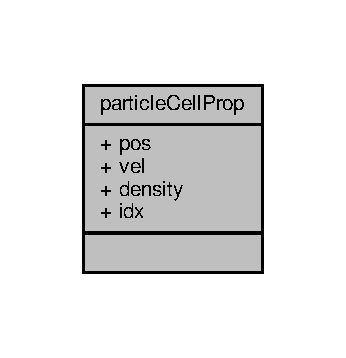
\includegraphics[width=166pt]{structparticle_cell_prop__coll__graph}
\end{center}
\end{figure}
\subsection*{Public Attributes}
\begin{DoxyCompactItemize}
\item 
\hypertarget{structparticle_cell_prop_a016a16c8e3e05c845ff225c15737cf2e}{float3 {\bfseries pos}}\label{structparticle_cell_prop_a016a16c8e3e05c845ff225c15737cf2e}

\item 
\hypertarget{structparticle_cell_prop_a2a2e5a1e900a4ef5635a7967c0049df3}{float3 {\bfseries vel}}\label{structparticle_cell_prop_a2a2e5a1e900a4ef5635a7967c0049df3}

\item 
\hypertarget{structparticle_cell_prop_a27ad7b6527abe273b0e4eb1d91e9b71c}{float {\bfseries density}}\label{structparticle_cell_prop_a27ad7b6527abe273b0e4eb1d91e9b71c}

\item 
\hypertarget{structparticle_cell_prop_ac32e55524eadd3499ccb99c0d04ef557}{int {\bfseries idx}}\label{structparticle_cell_prop_ac32e55524eadd3499ccb99c0d04ef557}

\end{DoxyCompactItemize}


\subsection{Detailed Description}
a structure to hold the properties of our particle cell 

The documentation for this struct was generated from the following file\-:\begin{DoxyCompactItemize}
\item 
include/\hyperlink{_cuda_s_p_h_kernals_8h}{Cuda\-S\-P\-H\-Kernals.\-h}\end{DoxyCompactItemize}

\hypertarget{classparticle_depth_frag}{\section{particle\-Depth\-Frag Class Reference}
\label{classparticle_depth_frag}\index{particle\-Depth\-Frag@{particle\-Depth\-Frag}}
}


Fragment shader for drawing point sprites as spheres. The output fragment will be the depth.  




Collaboration diagram for particle\-Depth\-Frag\-:\nopagebreak
\begin{figure}[H]
\begin{center}
\leavevmode
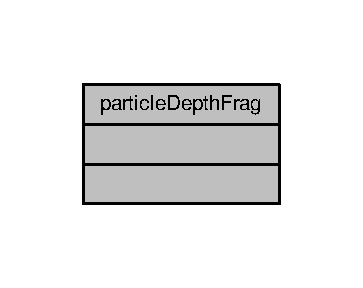
\includegraphics[width=174pt]{classparticle_depth_frag__coll__graph}
\end{center}
\end{figure}


\subsection{Detailed Description}
Fragment shader for drawing point sprites as spheres. The output fragment will be the depth. 

The documentation for this class was generated from the following file\-:\begin{DoxyCompactItemize}
\item 
shaders/\hyperlink{particle_depth_frag_8glsl}{particle\-Depth\-Frag.\-glsl}\end{DoxyCompactItemize}

\hypertarget{classparticle_depth_vert}{\section{particle\-Depth\-Vert Class Reference}
\label{classparticle_depth_vert}\index{particle\-Depth\-Vert@{particle\-Depth\-Vert}}
}


Vertex shader for our particle depth shader. Takes in points of particles and scales the point sprite with.  




\subsection{Detailed Description}
Vertex shader for our particle depth shader. Takes in points of particles and scales the point sprite with. 

the current scene projection matrix. 

The documentation for this class was generated from the following file\-:\begin{DoxyCompactItemize}
\item 
shaders/\hyperlink{particle_depth_vert_8glsl}{particle\-Depth\-Vert.\-glsl}\end{DoxyCompactItemize}

\hypertarget{structplane_prop}{\section{plane\-Prop Struct Reference}
\label{structplane_prop}\index{plane\-Prop@{plane\-Prop}}
}


a structure to hold the properties of our planes  




{\ttfamily \#include $<$Cuda\-S\-P\-H\-Kernals.\-h$>$}

\subsection*{Public Attributes}
\begin{DoxyCompactItemize}
\item 
\hypertarget{structplane_prop_a34453f09c8dbed51a1ac1c1cd5a610ea}{float3 {\bfseries pos}}\label{structplane_prop_a34453f09c8dbed51a1ac1c1cd5a610ea}

\item 
\hypertarget{structplane_prop_a4ed447d1e01222bd8b958ccd003d0563}{float3 {\bfseries normal}}\label{structplane_prop_a4ed447d1e01222bd8b958ccd003d0563}

\item 
\hypertarget{structplane_prop_a2d5b86467cb070520ede6dad51b0f2dc}{float {\bfseries rest\-Coef}}\label{structplane_prop_a2d5b86467cb070520ede6dad51b0f2dc}

\end{DoxyCompactItemize}


\subsection{Detailed Description}
a structure to hold the properties of our planes 

The documentation for this struct was generated from the following file\-:\begin{DoxyCompactItemize}
\item 
include/\hyperlink{_cuda_s_p_h_kernals_8h}{Cuda\-S\-P\-H\-Kernals.\-h}\end{DoxyCompactItemize}

\hypertarget{structqt__meta__stringdata___main_window__t}{\section{qt\-\_\-meta\-\_\-stringdata\-\_\-\-Main\-Window\-\_\-t Struct Reference}
\label{structqt__meta__stringdata___main_window__t}\index{qt\-\_\-meta\-\_\-stringdata\-\_\-\-Main\-Window\-\_\-t@{qt\-\_\-meta\-\_\-stringdata\-\_\-\-Main\-Window\-\_\-t}}
}
\subsection*{Public Attributes}
\begin{DoxyCompactItemize}
\item 
\hypertarget{structqt__meta__stringdata___main_window__t_a0a55531510dd06148b7b0f445e2b6c59}{Q\-Byte\-Array\-Data {\bfseries data} \mbox{[}3\mbox{]}}\label{structqt__meta__stringdata___main_window__t_a0a55531510dd06148b7b0f445e2b6c59}

\item 
\hypertarget{structqt__meta__stringdata___main_window__t_a3d76efa0e7bbfe9e02dc76fa032cd0e5}{char {\bfseries stringdata} \mbox{[}26\mbox{]}}\label{structqt__meta__stringdata___main_window__t_a3d76efa0e7bbfe9e02dc76fa032cd0e5}

\end{DoxyCompactItemize}


The documentation for this struct was generated from the following file\-:\begin{DoxyCompactItemize}
\item 
moc/moc\-\_\-mainwindow.\-cpp\end{DoxyCompactItemize}

\hypertarget{structqt__meta__stringdata___open_g_l_widget__t}{\section{qt\-\_\-meta\-\_\-stringdata\-\_\-\-Open\-G\-L\-Widget\-\_\-t Struct Reference}
\label{structqt__meta__stringdata___open_g_l_widget__t}\index{qt\-\_\-meta\-\_\-stringdata\-\_\-\-Open\-G\-L\-Widget\-\_\-t@{qt\-\_\-meta\-\_\-stringdata\-\_\-\-Open\-G\-L\-Widget\-\_\-t}}
}


Collaboration diagram for qt\-\_\-meta\-\_\-stringdata\-\_\-\-Open\-G\-L\-Widget\-\_\-t\-:\nopagebreak
\begin{figure}[H]
\begin{center}
\leavevmode
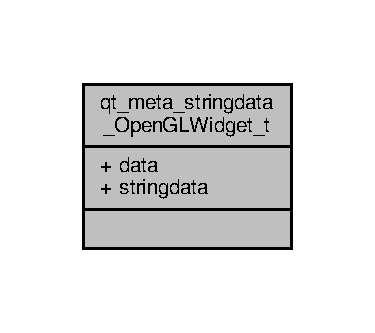
\includegraphics[width=180pt]{structqt__meta__stringdata___open_g_l_widget__t__coll__graph}
\end{center}
\end{figure}
\subsection*{Public Attributes}
\begin{DoxyCompactItemize}
\item 
\hypertarget{structqt__meta__stringdata___open_g_l_widget__t_ad12a546ae59866732c758206e9e72938}{Q\-Byte\-Array\-Data {\bfseries data} \mbox{[}48\mbox{]}}\label{structqt__meta__stringdata___open_g_l_widget__t_ad12a546ae59866732c758206e9e72938}

\item 
\hypertarget{structqt__meta__stringdata___open_g_l_widget__t_a356daa95022344d6aa7de96775220623}{char {\bfseries stringdata} \mbox{[}517\mbox{]}}\label{structqt__meta__stringdata___open_g_l_widget__t_a356daa95022344d6aa7de96775220623}

\end{DoxyCompactItemize}


The documentation for this struct was generated from the following file\-:\begin{DoxyCompactItemize}
\item 
/home/dexternation/\-A\-G\-S\-D\-T\-Fluid\-Sim/moc/moc\-\_\-\-Open\-G\-L\-Widget.\-cpp\end{DoxyCompactItemize}

\hypertarget{classsky_box_frag}{\section{sky\-Box\-Frag Class Reference}
\label{classsky_box_frag}\index{sky\-Box\-Frag@{sky\-Box\-Frag}}
}


Fragment shader for our shy box shader.  




\subsection{Detailed Description}
Fragment shader for our shy box shader. 

The documentation for this class was generated from the following file\-:\begin{DoxyCompactItemize}
\item 
shaders/\hyperlink{sky_box_frag_8glsl}{sky\-Box\-Frag.\-glsl}\end{DoxyCompactItemize}

\hypertarget{classsky_box_vert}{\section{sky\-Box\-Vert Class Reference}
\label{classsky_box_vert}\index{sky\-Box\-Vert@{sky\-Box\-Vert}}
}


Vertex shader for our sky box shader. Just passes through positions and tex coords and positions.  




Collaboration diagram for sky\-Box\-Vert\-:\nopagebreak
\begin{figure}[H]
\begin{center}
\leavevmode
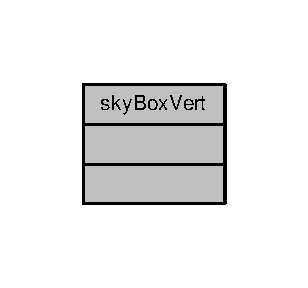
\includegraphics[width=148pt]{classsky_box_vert__coll__graph}
\end{center}
\end{figure}


\subsection{Detailed Description}
Vertex shader for our sky box shader. Just passes through positions and tex coords and positions. 

The documentation for this class was generated from the following file\-:\begin{DoxyCompactItemize}
\item 
/home/dexternation/\-A\-G\-S\-D\-T\-Fluid\-Sim/shaders/\hyperlink{sky_box_vert_8glsl}{sky\-Box\-Vert.\-glsl}\end{DoxyCompactItemize}

\hypertarget{class_s_p_h_engine}{\section{S\-P\-H\-Engine Class Reference}
\label{class_s_p_h_engine}\index{S\-P\-H\-Engine@{S\-P\-H\-Engine}}
}


our cuda libraries  




{\ttfamily \#include $<$S\-P\-H\-Engine.\-h$>$}

\subsection*{Public Member Functions}
\begin{DoxyCompactItemize}
\item 
\hyperlink{class_s_p_h_engine_a8be3b3f99242c3548ade6ff9314fc46c}{S\-P\-H\-Engine} (unsigned int \-\_\-num\-Particles=0, float \-\_\-mass=10.f, float \-\_\-density=998.\-2f, float \-\_\-contaner\-Size=10)
\begin{DoxyCompactList}\small\item\em defualt constructor \end{DoxyCompactList}\item 
\hypertarget{class_s_p_h_engine_a0969407c141667c1147d409a0397257d}{\hyperlink{class_s_p_h_engine_a0969407c141667c1147d409a0397257d}{$\sim$\-S\-P\-H\-Engine} ()}\label{class_s_p_h_engine_a0969407c141667c1147d409a0397257d}

\begin{DoxyCompactList}\small\item\em default destructor \end{DoxyCompactList}\item 
\hypertarget{class_s_p_h_engine_a0df6d1b33d50afb152e2992de5af5700}{void \hyperlink{class_s_p_h_engine_a0df6d1b33d50afb152e2992de5af5700}{init} ()}\label{class_s_p_h_engine_a0df6d1b33d50afb152e2992de5af5700}

\begin{DoxyCompactList}\small\item\em Initialises our class. This allocates all memory needed for the simulation. \end{DoxyCompactList}\item 
void \hyperlink{class_s_p_h_engine_a1a17b5c04756850b68cf95b917019241}{update} (float \-\_\-time\-Step)
\begin{DoxyCompactList}\small\item\em updates our particles positions with navier-\/stokes equations based on timestep of the update. \end{DoxyCompactList}\item 
\hypertarget{class_s_p_h_engine_a91f224d67175615716059dba23c38a98}{void \hyperlink{class_s_p_h_engine_a91f224d67175615716059dba23c38a98}{draw\-Arrays} ()}\label{class_s_p_h_engine_a91f224d67175615716059dba23c38a98}

\begin{DoxyCompactList}\small\item\em Draws our V\-A\-O. This contatins a buffer of positions mapped to vertex\-Attri\-B\-Array 0. \end{DoxyCompactList}\item 
\hypertarget{class_s_p_h_engine_aee51f7802e02c838732d9acab37da89a}{G\-Luint \hyperlink{class_s_p_h_engine_aee51f7802e02c838732d9acab37da89a}{get\-Position\-Buffer} ()}\label{class_s_p_h_engine_aee51f7802e02c838732d9acab37da89a}

\begin{DoxyCompactList}\small\item\em returns the output postion open\-G\-L buffer of our particles \end{DoxyCompactList}\item 
\hypertarget{class_s_p_h_engine_acbc638f7ab8fa2ab356dadf677df10c6}{void \hyperlink{class_s_p_h_engine_acbc638f7ab8fa2ab356dadf677df10c6}{set\-Desity} (float \-\_\-density)}\label{class_s_p_h_engine_acbc638f7ab8fa2ab356dadf677df10c6}

\begin{DoxyCompactList}\small\item\em Mutator for the desity of our fluid. \end{DoxyCompactList}\item 
\hypertarget{class_s_p_h_engine_a8ee29d26f9451d81a07abde5b1aa53c6}{float \hyperlink{class_s_p_h_engine_a8ee29d26f9451d81a07abde5b1aa53c6}{get\-Density} ()}\label{class_s_p_h_engine_a8ee29d26f9451d81a07abde5b1aa53c6}

\begin{DoxyCompactList}\small\item\em accessor to query the density of our fluid \end{DoxyCompactList}\item 
\hypertarget{class_s_p_h_engine_a0f937d1c09511f302455f102fae167c3}{void \hyperlink{class_s_p_h_engine_a0f937d1c09511f302455f102fae167c3}{set\-Particle\-Mass} (float \-\_\-mass)}\label{class_s_p_h_engine_a0f937d1c09511f302455f102fae167c3}

\begin{DoxyCompactList}\small\item\em mutator to set the mass of our fluid particles \end{DoxyCompactList}\item 
\hypertarget{class_s_p_h_engine_a196e04ba23d9d9c73924f3af8a8240ed}{void \hyperlink{class_s_p_h_engine_a196e04ba23d9d9c73924f3af8a8240ed}{set\-Smoothing\-Length} (float \-\_\-length)}\label{class_s_p_h_engine_a196e04ba23d9d9c73924f3af8a8240ed}

\begin{DoxyCompactList}\small\item\em Mutator for the smoothing length of our simulation. Can also be thought of as hash cell size. \end{DoxyCompactList}\item 
\hypertarget{class_s_p_h_engine_a5eebbb4eaf3c773e263396d49a76fc3e}{float \hyperlink{class_s_p_h_engine_a5eebbb4eaf3c773e263396d49a76fc3e}{get\-Smoothing\-Length} ()}\label{class_s_p_h_engine_a5eebbb4eaf3c773e263396d49a76fc3e}

\begin{DoxyCompactList}\small\item\em accessor to query the smoothing length of our fluid \end{DoxyCompactList}\item 
\hypertarget{class_s_p_h_engine_a293fc06859e21473b03626a55c5c3a69}{void \hyperlink{class_s_p_h_engine_a293fc06859e21473b03626a55c5c3a69}{set\-Gas\-Constant} (float \-\_\-gas\-Const)}\label{class_s_p_h_engine_a293fc06859e21473b03626a55c5c3a69}

\begin{DoxyCompactList}\small\item\em Mutator for the gas constant of our fluid. \end{DoxyCompactList}\item 
\hypertarget{class_s_p_h_engine_a683d29b540672f364c306b304bd50ea7}{float \hyperlink{class_s_p_h_engine_a683d29b540672f364c306b304bd50ea7}{get\-Gas\-Const} ()}\label{class_s_p_h_engine_a683d29b540672f364c306b304bd50ea7}

\begin{DoxyCompactList}\small\item\em accessor to query the gas constant of our fluid \end{DoxyCompactList}\item 
\hypertarget{class_s_p_h_engine_a296c06a01cb0a93dfa150c3acea64493}{void \hyperlink{class_s_p_h_engine_a296c06a01cb0a93dfa150c3acea64493}{set\-Visc\-Coef} (float \-\_\-visc\-Coef)}\label{class_s_p_h_engine_a296c06a01cb0a93dfa150c3acea64493}

\begin{DoxyCompactList}\small\item\em Mutator for our viscosity coeficient of our fluid. \end{DoxyCompactList}\item 
\hypertarget{class_s_p_h_engine_a6d3709693af1379db5b60b02171d8c8b}{float \hyperlink{class_s_p_h_engine_a6d3709693af1379db5b60b02171d8c8b}{get\-Visc\-Coef} ()}\label{class_s_p_h_engine_a6d3709693af1379db5b60b02171d8c8b}

\begin{DoxyCompactList}\small\item\em accessor to query the viscosity coeficient of our fluid \end{DoxyCompactList}\item 
\hypertarget{class_s_p_h_engine_ac1e6f83f2da1ec79a6e6a633b810daba}{void \hyperlink{class_s_p_h_engine_ac1e6f83f2da1ec79a6e6a633b810daba}{set\-Tension\-Coef} (float \-\_\-tens\-Coef)}\label{class_s_p_h_engine_ac1e6f83f2da1ec79a6e6a633b810daba}

\begin{DoxyCompactList}\small\item\em mutation for our tension coeficient of our fluid \end{DoxyCompactList}\item 
\hypertarget{class_s_p_h_engine_afa874402b050ea1f618bf2caf7f988b4}{float \hyperlink{class_s_p_h_engine_afa874402b050ea1f618bf2caf7f988b4}{get\-Tension\-Coef} ()}\label{class_s_p_h_engine_afa874402b050ea1f618bf2caf7f988b4}

\begin{DoxyCompactList}\small\item\em accessor to query our tension coeficient of our fluid \end{DoxyCompactList}\item 
\hypertarget{class_s_p_h_engine_a6b418198ceab591b1abfa5f645dbc9d7}{void \hyperlink{class_s_p_h_engine_a6b418198ceab591b1abfa5f645dbc9d7}{set\-Vel\-Cor\-Coef} (float \-\_\-vel\-Cor\-Coef)}\label{class_s_p_h_engine_a6b418198ceab591b1abfa5f645dbc9d7}

\begin{DoxyCompactList}\small\item\em mutator to our velocity correction \end{DoxyCompactList}\item 
void \hyperlink{class_s_p_h_engine_aad9d9bc9a1a7e5f64a5e045c339f8b3e}{set\-Max\-Num\-Samples} (int \-\_\-num\-Samples)
\begin{DoxyCompactList}\small\item\em mutator for our maximum number of samples per particle in our fluid solver \end{DoxyCompactList}\item 
void \hyperlink{class_s_p_h_engine_afe2b02e535cf064f91f2de4312c8ae39}{add\-Collision\-Object} (float3 \-\_\-min, float3 \-\_\-max, float3 \-\_\-rest\-Coef, bool \-\_\-is\-Container)
\begin{DoxyCompactList}\small\item\em adds a colllision object for our fluid. So far supports containers and collision cuboids \end{DoxyCompactList}\item 
\hypertarget{class_s_p_h_engine_a387ab48532ca20b2eb31319e862e243b}{int \hyperlink{class_s_p_h_engine_a387ab48532ca20b2eb31319e862e243b}{get\-Num\-Particles} ()}\label{class_s_p_h_engine_a387ab48532ca20b2eb31319e862e243b}

\begin{DoxyCompactList}\small\item\em accessor to number of particles in simulation \end{DoxyCompactList}\item 
\hypertarget{class_s_p_h_engine_a692ed8ae0cdb67f4a774fa2a94ad635f}{void \hyperlink{class_s_p_h_engine_a692ed8ae0cdb67f4a774fa2a94ad635f}{signal\-Reset} ()}\label{class_s_p_h_engine_a692ed8ae0cdb67f4a774fa2a94ad635f}

\begin{DoxyCompactList}\small\item\em signals our engine to reset the simulation \end{DoxyCompactList}\item 
void \hyperlink{class_s_p_h_engine_a4e61b1f56e20ab4eee7edd111c59912f}{signal\-Add\-Particles} (int \-\_\-num\-Particles)
\begin{DoxyCompactList}\small\item\em signals the engine to add particles to our simulation \end{DoxyCompactList}\item 
void \hyperlink{class_s_p_h_engine_a130606677b2c3edbc9b95006672c1578}{set\-Spawn\-Box\-Pos} (float \-\_\-x, float \-\_\-y, float \-\_\-z)
\begin{DoxyCompactList}\small\item\em sets the spawn box position \end{DoxyCompactList}\item 
float3 \hyperlink{class_s_p_h_engine_a452295b33bfa893db3c9484da9ce9fb5}{get\-Spawn\-Box\-Pos} ()
\begin{DoxyCompactList}\small\item\em accessor to our spawn box position \end{DoxyCompactList}\item 
void \hyperlink{class_s_p_h_engine_a2bf5d2bc9fc8bcc39d42108150123663}{set\-Spawn\-Box\-Size} (float \-\_\-size)
\begin{DoxyCompactList}\small\item\em set the size of our spawn box \end{DoxyCompactList}\item 
float \hyperlink{class_s_p_h_engine_a234554f5b25de8cc34541e1fd0a4b52b}{get\-Spawn\-Box\-Size} ()
\begin{DoxyCompactList}\small\item\em accessor to our spawn box size \end{DoxyCompactList}\end{DoxyCompactItemize}


\subsection{Detailed Description}
our cuda libraries 

This class uses cuda and parralel algorithms to manage particles in a fluid simulation.

our S\-P\-H kernals

\begin{DoxyAuthor}{Author}
Declan Russell 
\end{DoxyAuthor}
\begin{DoxyDate}{Date}
09/03/2015 
\end{DoxyDate}
\begin{DoxyVersion}{Version}
1.\-0 Our fluid simulation uses smoothed particle hydrodynamics and true navier stokes equations to compute our particle positions in our simulation. This class also manages its own open\-G\-L buffer storing postions of particles in vertex attrip pointer 0. In case you wish to draw these particles. 
\end{DoxyVersion}


\subsection{Constructor \& Destructor Documentation}
\hypertarget{class_s_p_h_engine_a8be3b3f99242c3548ade6ff9314fc46c}{\index{S\-P\-H\-Engine@{S\-P\-H\-Engine}!S\-P\-H\-Engine@{S\-P\-H\-Engine}}
\index{S\-P\-H\-Engine@{S\-P\-H\-Engine}!SPHEngine@{S\-P\-H\-Engine}}
\subsubsection[{S\-P\-H\-Engine}]{\setlength{\rightskip}{0pt plus 5cm}S\-P\-H\-Engine\-::\-S\-P\-H\-Engine (
\begin{DoxyParamCaption}
\item[{unsigned int}]{\-\_\-num\-Particles = {\ttfamily 0}, }
\item[{float}]{\-\_\-mass = {\ttfamily 10.f}, }
\item[{float}]{\-\_\-density = {\ttfamily 998.2f}, }
\item[{float}]{\-\_\-contaner\-Size = {\ttfamily 10}}
\end{DoxyParamCaption}
)}}\label{class_s_p_h_engine_a8be3b3f99242c3548ade6ff9314fc46c}


defualt constructor 


\begin{DoxyParams}{Parameters}
{\em \-\_\-num\-Particles} & how many particles we want to have on simulation initialisation. \\
\hline
{\em \-\_\-mass} & -\/ mass per partilce of our fluid \\
\hline
{\em \-\_\-density} & -\/ the density of our fluid \\
\hline
{\em \-\_\-contaner\-Size} & -\/ the contaner size of for our fluid. e.\-g. 1 is a cube of 1$\ast$1$\ast$1. \\
\hline
\end{DoxyParams}


\subsection{Member Function Documentation}
\hypertarget{class_s_p_h_engine_afe2b02e535cf064f91f2de4312c8ae39}{\index{S\-P\-H\-Engine@{S\-P\-H\-Engine}!add\-Collision\-Object@{add\-Collision\-Object}}
\index{add\-Collision\-Object@{add\-Collision\-Object}!SPHEngine@{S\-P\-H\-Engine}}
\subsubsection[{add\-Collision\-Object}]{\setlength{\rightskip}{0pt plus 5cm}void S\-P\-H\-Engine\-::add\-Collision\-Object (
\begin{DoxyParamCaption}
\item[{float3}]{\-\_\-min, }
\item[{float3}]{\-\_\-max, }
\item[{float3}]{\-\_\-rest\-Coef, }
\item[{bool}]{\-\_\-is\-Container}
\end{DoxyParamCaption}
)}}\label{class_s_p_h_engine_afe2b02e535cf064f91f2de4312c8ae39}


adds a colllision object for our fluid. So far supports containers and collision cuboids 

\begin{DoxyWarning}{Warning}
Very simple A\-A\-B\-B collision. Probably rubish and unoptimized 
\end{DoxyWarning}

\begin{DoxyParams}{Parameters}
{\em \-\_\-min} & -\/ container minimum \\
\hline
{\em \-\_\-max} & -\/ container maximum \\
\hline
{\em \-\_\-rest\-Coef} & -\/ coeficient of restitution of our container in our 3 axis \\
\hline
{\em \-\_\-is\-Container} & -\/ indicate whether or not we are adding a container of a box \\
\hline
\end{DoxyParams}
\hypertarget{class_s_p_h_engine_a452295b33bfa893db3c9484da9ce9fb5}{\index{S\-P\-H\-Engine@{S\-P\-H\-Engine}!get\-Spawn\-Box\-Pos@{get\-Spawn\-Box\-Pos}}
\index{get\-Spawn\-Box\-Pos@{get\-Spawn\-Box\-Pos}!SPHEngine@{S\-P\-H\-Engine}}
\subsubsection[{get\-Spawn\-Box\-Pos}]{\setlength{\rightskip}{0pt plus 5cm}float3 S\-P\-H\-Engine\-::get\-Spawn\-Box\-Pos (
\begin{DoxyParamCaption}
{}
\end{DoxyParamCaption}
)\hspace{0.3cm}{\ttfamily [inline]}}}\label{class_s_p_h_engine_a452295b33bfa893db3c9484da9ce9fb5}


accessor to our spawn box position 

\begin{DoxyReturn}{Returns}
float3 spawn box position 
\end{DoxyReturn}
\hypertarget{class_s_p_h_engine_a234554f5b25de8cc34541e1fd0a4b52b}{\index{S\-P\-H\-Engine@{S\-P\-H\-Engine}!get\-Spawn\-Box\-Size@{get\-Spawn\-Box\-Size}}
\index{get\-Spawn\-Box\-Size@{get\-Spawn\-Box\-Size}!SPHEngine@{S\-P\-H\-Engine}}
\subsubsection[{get\-Spawn\-Box\-Size}]{\setlength{\rightskip}{0pt plus 5cm}float S\-P\-H\-Engine\-::get\-Spawn\-Box\-Size (
\begin{DoxyParamCaption}
{}
\end{DoxyParamCaption}
)\hspace{0.3cm}{\ttfamily [inline]}}}\label{class_s_p_h_engine_a234554f5b25de8cc34541e1fd0a4b52b}


accessor to our spawn box size 

\begin{DoxyReturn}{Returns}
float spawn box size 
\end{DoxyReturn}
\hypertarget{class_s_p_h_engine_aad9d9bc9a1a7e5f64a5e045c339f8b3e}{\index{S\-P\-H\-Engine@{S\-P\-H\-Engine}!set\-Max\-Num\-Samples@{set\-Max\-Num\-Samples}}
\index{set\-Max\-Num\-Samples@{set\-Max\-Num\-Samples}!SPHEngine@{S\-P\-H\-Engine}}
\subsubsection[{set\-Max\-Num\-Samples}]{\setlength{\rightskip}{0pt plus 5cm}void S\-P\-H\-Engine\-::set\-Max\-Num\-Samples (
\begin{DoxyParamCaption}
\item[{int}]{\-\_\-num\-Samples}
\end{DoxyParamCaption}
)\hspace{0.3cm}{\ttfamily [inline]}}}\label{class_s_p_h_engine_aad9d9bc9a1a7e5f64a5e045c339f8b3e}


mutator for our maximum number of samples per particle in our fluid solver 


\begin{DoxyParams}{Parameters}
{\em \-\_\-num\-Samples} & -\/ desired maximum number of samples per particle in fluid solver \\
\hline
\end{DoxyParams}
\hypertarget{class_s_p_h_engine_a130606677b2c3edbc9b95006672c1578}{\index{S\-P\-H\-Engine@{S\-P\-H\-Engine}!set\-Spawn\-Box\-Pos@{set\-Spawn\-Box\-Pos}}
\index{set\-Spawn\-Box\-Pos@{set\-Spawn\-Box\-Pos}!SPHEngine@{S\-P\-H\-Engine}}
\subsubsection[{set\-Spawn\-Box\-Pos}]{\setlength{\rightskip}{0pt plus 5cm}void S\-P\-H\-Engine\-::set\-Spawn\-Box\-Pos (
\begin{DoxyParamCaption}
\item[{float}]{\-\_\-x, }
\item[{float}]{\-\_\-y, }
\item[{float}]{\-\_\-z}
\end{DoxyParamCaption}
)\hspace{0.3cm}{\ttfamily [inline]}}}\label{class_s_p_h_engine_a130606677b2c3edbc9b95006672c1578}


sets the spawn box position 


\begin{DoxyParams}{Parameters}
{\em \-\_\-x} & -\/ x position of spawn box \\
\hline
{\em \-\_\-y} & -\/ y position of spawn box \\
\hline
{\em \-\_\-z} & -\/ z position of spawn box \\
\hline
\end{DoxyParams}
\hypertarget{class_s_p_h_engine_a2bf5d2bc9fc8bcc39d42108150123663}{\index{S\-P\-H\-Engine@{S\-P\-H\-Engine}!set\-Spawn\-Box\-Size@{set\-Spawn\-Box\-Size}}
\index{set\-Spawn\-Box\-Size@{set\-Spawn\-Box\-Size}!SPHEngine@{S\-P\-H\-Engine}}
\subsubsection[{set\-Spawn\-Box\-Size}]{\setlength{\rightskip}{0pt plus 5cm}void S\-P\-H\-Engine\-::set\-Spawn\-Box\-Size (
\begin{DoxyParamCaption}
\item[{float}]{\-\_\-size}
\end{DoxyParamCaption}
)\hspace{0.3cm}{\ttfamily [inline]}}}\label{class_s_p_h_engine_a2bf5d2bc9fc8bcc39d42108150123663}


set the size of our spawn box 


\begin{DoxyParams}{Parameters}
{\em \-\_\-size} & -\/ the size of our spawn box \\
\hline
\end{DoxyParams}
\hypertarget{class_s_p_h_engine_a4e61b1f56e20ab4eee7edd111c59912f}{\index{S\-P\-H\-Engine@{S\-P\-H\-Engine}!signal\-Add\-Particles@{signal\-Add\-Particles}}
\index{signal\-Add\-Particles@{signal\-Add\-Particles}!SPHEngine@{S\-P\-H\-Engine}}
\subsubsection[{signal\-Add\-Particles}]{\setlength{\rightskip}{0pt plus 5cm}void S\-P\-H\-Engine\-::signal\-Add\-Particles (
\begin{DoxyParamCaption}
\item[{int}]{\-\_\-num\-Particles}
\end{DoxyParamCaption}
)}}\label{class_s_p_h_engine_a4e61b1f56e20ab4eee7edd111c59912f}


signals the engine to add particles to our simulation 


\begin{DoxyParams}{Parameters}
{\em \-\_\-num\-Particles} & -\/ the number of particles to add to our simulation \\
\hline
\end{DoxyParams}
\hypertarget{class_s_p_h_engine_a1a17b5c04756850b68cf95b917019241}{\index{S\-P\-H\-Engine@{S\-P\-H\-Engine}!update@{update}}
\index{update@{update}!SPHEngine@{S\-P\-H\-Engine}}
\subsubsection[{update}]{\setlength{\rightskip}{0pt plus 5cm}void S\-P\-H\-Engine\-::update (
\begin{DoxyParamCaption}
\item[{float}]{\-\_\-time\-Step}
\end{DoxyParamCaption}
)}}\label{class_s_p_h_engine_a1a17b5c04756850b68cf95b917019241}


updates our particles positions with navier-\/stokes equations based on timestep of the update. 


\begin{DoxyParams}{Parameters}
{\em \-\_\-time\-Step} & -\/ the timestep we wish to update our particles with. \\
\hline
\end{DoxyParams}


The documentation for this class was generated from the following files\-:\begin{DoxyCompactItemize}
\item 
include/\hyperlink{_s_p_h_engine_8h}{S\-P\-H\-Engine.\-h}\item 
src/S\-P\-H\-Engine.\-cpp\end{DoxyCompactItemize}

\hypertarget{classthickness_frag}{\section{thickness\-Frag Class Reference}
\label{classthickness_frag}\index{thickness\-Frag@{thickness\-Frag}}
}


Fragment shader to output the thickness of our fluid. It is important for you to run this with.  




\subsection{Detailed Description}
Fragment shader to output the thickness of our fluid. It is important for you to run this with. 

additive blending and no depth test for it to work. The more items that are drawn on top of each other then the thicker the fluid. 

The documentation for this class was generated from the following file\-:\begin{DoxyCompactItemize}
\item 
shaders/\hyperlink{thickness_frag_8glsl}{thickness\-Frag.\-glsl}\end{DoxyCompactItemize}

\hypertarget{classthickness_vert}{\section{thickness\-Vert Class Reference}
\label{classthickness_vert}\index{thickness\-Vert@{thickness\-Vert}}
}


Vertex shader for our thickness shader. Takes in points of particles and scales the point sprite with.  




Collaboration diagram for thickness\-Vert\-:\nopagebreak
\begin{figure}[H]
\begin{center}
\leavevmode
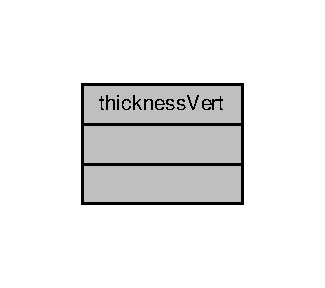
\includegraphics[width=156pt]{classthickness_vert__coll__graph}
\end{center}
\end{figure}


\subsection{Detailed Description}
Vertex shader for our thickness shader. Takes in points of particles and scales the point sprite with. 

the current scene projection matrix. 

The documentation for this class was generated from the following file\-:\begin{DoxyCompactItemize}
\item 
/home/dexternation/\-A\-G\-S\-D\-T\-Fluid\-Sim/shaders/\hyperlink{thickness_vert_8glsl}{thickness\-Vert.\-glsl}\end{DoxyCompactItemize}

\hypertarget{class_ui___main_window}{\section{Ui\-\_\-\-Main\-Window Class Reference}
\label{class_ui___main_window}\index{Ui\-\_\-\-Main\-Window@{Ui\-\_\-\-Main\-Window}}
}


Inheritance diagram for Ui\-\_\-\-Main\-Window\-:\nopagebreak
\begin{figure}[H]
\begin{center}
\leavevmode
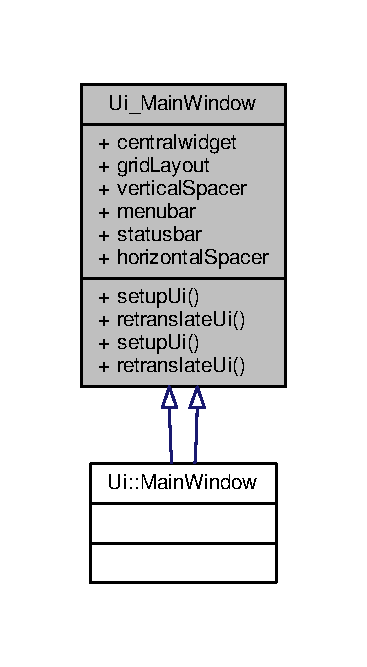
\includegraphics[width=176pt]{class_ui___main_window__inherit__graph}
\end{center}
\end{figure}


Collaboration diagram for Ui\-\_\-\-Main\-Window\-:\nopagebreak
\begin{figure}[H]
\begin{center}
\leavevmode
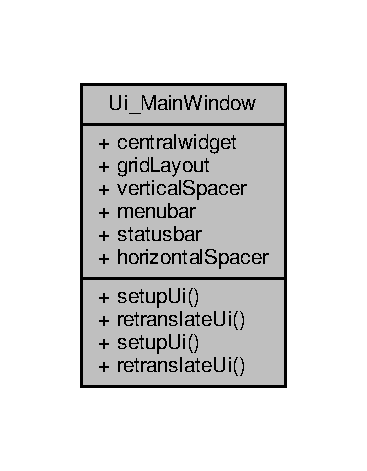
\includegraphics[width=176pt]{class_ui___main_window__coll__graph}
\end{center}
\end{figure}
\subsection*{Public Member Functions}
\begin{DoxyCompactItemize}
\item 
\hypertarget{class_ui___main_window_acf4a0872c4c77d8f43a2ec66ed849b58}{void {\bfseries setup\-Ui} (Q\-Main\-Window $\ast$\hyperlink{class_main_window}{Main\-Window})}\label{class_ui___main_window_acf4a0872c4c77d8f43a2ec66ed849b58}

\item 
\hypertarget{class_ui___main_window_a097dd160c3534a204904cb374412c618}{void {\bfseries retranslate\-Ui} (Q\-Main\-Window $\ast$\hyperlink{class_main_window}{Main\-Window})}\label{class_ui___main_window_a097dd160c3534a204904cb374412c618}

\item 
\hypertarget{class_ui___main_window_acf4a0872c4c77d8f43a2ec66ed849b58}{void {\bfseries setup\-Ui} (Q\-Main\-Window $\ast$\hyperlink{class_main_window}{Main\-Window})}\label{class_ui___main_window_acf4a0872c4c77d8f43a2ec66ed849b58}

\item 
\hypertarget{class_ui___main_window_a097dd160c3534a204904cb374412c618}{void {\bfseries retranslate\-Ui} (Q\-Main\-Window $\ast$\hyperlink{class_main_window}{Main\-Window})}\label{class_ui___main_window_a097dd160c3534a204904cb374412c618}

\end{DoxyCompactItemize}
\subsection*{Public Attributes}
\begin{DoxyCompactItemize}
\item 
\hypertarget{class_ui___main_window_a39420100bfee3ba57f137af5a3b0f8e9}{Q\-Widget $\ast$ {\bfseries centralwidget}}\label{class_ui___main_window_a39420100bfee3ba57f137af5a3b0f8e9}

\item 
\hypertarget{class_ui___main_window_ac4586abe48f0aabf940b0dc2df3772ed}{Q\-Grid\-Layout $\ast$ {\bfseries grid\-Layout}}\label{class_ui___main_window_ac4586abe48f0aabf940b0dc2df3772ed}

\item 
\hypertarget{class_ui___main_window_a8384329c3663ff274e926a12024aab52}{Q\-Spacer\-Item $\ast$ {\bfseries vertical\-Spacer}}\label{class_ui___main_window_a8384329c3663ff274e926a12024aab52}

\item 
\hypertarget{class_ui___main_window_a734b1d3bb71c1b8e1ea01b7fa4344fce}{Q\-Menu\-Bar $\ast$ {\bfseries menubar}}\label{class_ui___main_window_a734b1d3bb71c1b8e1ea01b7fa4344fce}

\item 
\hypertarget{class_ui___main_window_a07519bbb9a350befd6feb4e84ef299fd}{Q\-Status\-Bar $\ast$ {\bfseries statusbar}}\label{class_ui___main_window_a07519bbb9a350befd6feb4e84ef299fd}

\item 
\hypertarget{class_ui___main_window_a7871ea8c4b6c595d7ccd53960b344719}{Q\-Spacer\-Item $\ast$ {\bfseries horizontal\-Spacer}}\label{class_ui___main_window_a7871ea8c4b6c595d7ccd53960b344719}

\end{DoxyCompactItemize}


The documentation for this class was generated from the following file\-:\begin{DoxyCompactItemize}
\item 
/home/dexternation/\-A\-G\-S\-D\-T\-Fluid\-Sim/include/ui\-\_\-mainwindow.\-h\end{DoxyCompactItemize}

\chapter{File Documentation}
\hypertarget{_cuda_s_p_h_kernals_8cu}{\section{/home/dexternation/\-A\-G\-S\-D\-T\-Fluid\-Sim/cuda\-Src/\-Cuda\-S\-P\-H\-Kernals.cu File Reference}
\label{_cuda_s_p_h_kernals_8cu}\index{/home/dexternation/\-A\-G\-S\-D\-T\-Fluid\-Sim/cuda\-Src/\-Cuda\-S\-P\-H\-Kernals.\-cu@{/home/dexternation/\-A\-G\-S\-D\-T\-Fluid\-Sim/cuda\-Src/\-Cuda\-S\-P\-H\-Kernals.\-cu}}
}
{\ttfamily \#include $<$thrust/sort.\-h$>$}\\*
{\ttfamily \#include $<$thrust/fill.\-h$>$}\\*
{\ttfamily \#include $<$thrust/device\-\_\-ptr.\-h$>$}\\*
{\ttfamily \#include $<$thrust/scan.\-h$>$}\\*
{\ttfamily \#include \char`\"{}Cuda\-S\-P\-H\-Kernals.\-h\char`\"{}}\\*
{\ttfamily \#include \char`\"{}helper\-\_\-math.\-h\char`\"{}}\\*
Include dependency graph for Cuda\-S\-P\-H\-Kernals.\-cu\-:\nopagebreak
\begin{figure}[H]
\begin{center}
\leavevmode
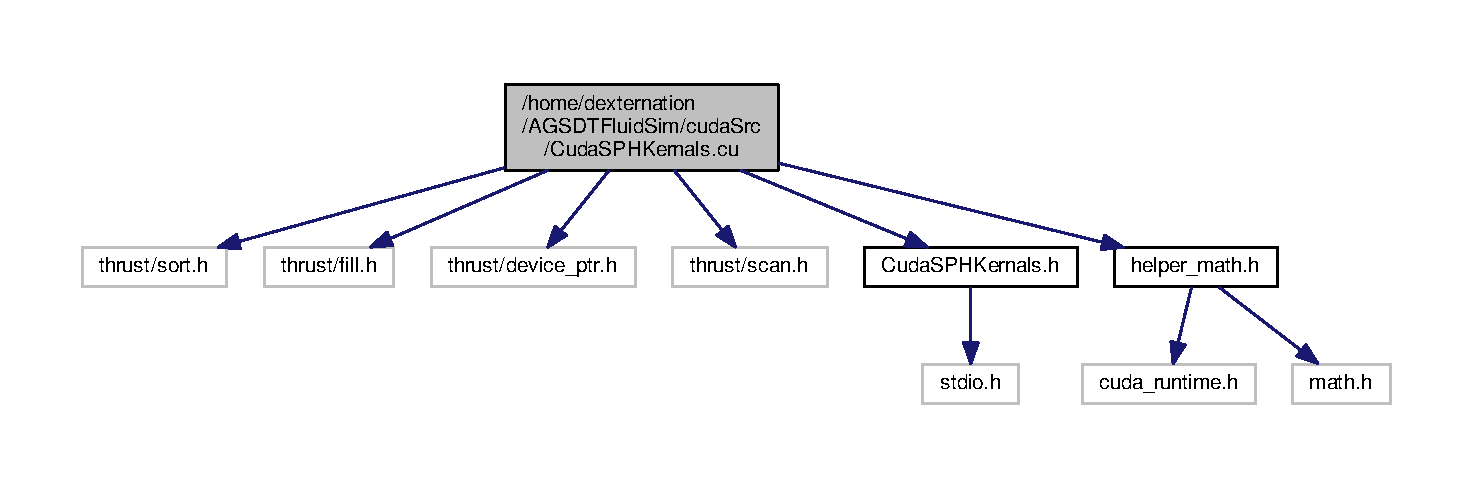
\includegraphics[width=350pt]{_cuda_s_p_h_kernals_8cu__incl}
\end{center}
\end{figure}
\subsection*{Macros}
\begin{DoxyCompactItemize}
\item 
\hypertarget{_cuda_s_p_h_kernals_8cu_a1daf785e3f68d293c7caa1c756d5cb74}{\#define {\bfseries pi}~3.\-14159265359f}\label{_cuda_s_p_h_kernals_8cu_a1daf785e3f68d293c7caa1c756d5cb74}

\end{DoxyCompactItemize}
\subsection*{Functions}
\begin{DoxyCompactItemize}
\item 
\-\_\-\-\_\-global\-\_\-\-\_\- void \hyperlink{_cuda_s_p_h_kernals_8cu_afdcbd8ca539116cc7b8d030b1e418e77}{point\-Hash} (unsigned int $\ast$d\-\_\-hash\-Array, float3 $\ast$d\-\_\-pos\-Array, unsigned int num\-Particles, float resolution, float \-\_\-grid\-Scaler)
\begin{DoxyCompactList}\small\item\em Kernal designed to produce a has key based on the location of a particle. \end{DoxyCompactList}\item 
\-\_\-\-\_\-global\-\_\-\-\_\- void \hyperlink{_cuda_s_p_h_kernals_8cu_ad805b6eb0d36394de57c25b3d06718ca}{count\-Cell\-Occ\-Kernal} (unsigned int $\ast$d\-\_\-hash\-Array, unsigned int $\ast$d\-\_\-cell\-Occ\-Array, int \-\_\-hash\-Table\-Size, unsigned int \-\_\-num\-Points)
\begin{DoxyCompactList}\small\item\em This kernal is designed to count the cell occpancy of a hash table. \end{DoxyCompactList}\item 
\-\_\-\-\_\-device\-\_\-\-\_\- float \hyperlink{_cuda_s_p_h_kernals_8cu_aaaee82afeb737d25fb86efb6949aa1b5}{density\-Weighting} (float \-\_\-dst, float \-\_\-smoothing\-Length, float \-\_\-dens\-Kern\-Const)
\begin{DoxyCompactList}\small\item\em This is our desity weighting kernal used in our navier stokes equations. \end{DoxyCompactList}\item 
\-\_\-\-\_\-device\-\_\-\-\_\- float3 \hyperlink{_cuda_s_p_h_kernals_8cu_ad44155cc5df4e6c30367f437d6fcb489}{pressure\-Weighting} (float3 \-\_\-r, float \-\_\-dst, float \-\_\-smoothing\-Length, float \-\_\-press\-Kern\-Const)
\begin{DoxyCompactList}\small\item\em This is our desity weighting kernal used in our navier stokes equations. \end{DoxyCompactList}\item 
\-\_\-\-\_\-device\-\_\-\-\_\- float3 \hyperlink{_cuda_s_p_h_kernals_8cu_ad682f881cf72f537f3cad1ba7993b5b5}{viscosity\-Weighting} (float3 \-\_\-r, float \-\_\-dst, float \-\_\-smoothing\-Length, float \-\_\-visc\-Kern\-Const)
\begin{DoxyCompactList}\small\item\em This is our viscosty weighting kernal used in our navier stokes equations. \end{DoxyCompactList}\item 
\hypertarget{_cuda_s_p_h_kernals_8cu_a8e6781d18982655b4efd3db1e6548a41}{\-\_\-\-\_\-global\-\_\-\-\_\- void {\bfseries fluid\-Solver\-Per\-Cell\-Kernal} (int \-\_\-max\-Samples, float3 $\ast$d\-\_\-pos\-Array, float3 $\ast$d\-\_\-vel\-Array, unsigned int $\ast$d\-\_\-cell\-Occ\-Array, unsigned int $\ast$d\-\_\-cell\-Indx\-Array, int \-\_\-hash\-Resolution, int \-\_\-hash\-Table\-Size, float \-\_\-smoothing\-Length, float \-\_\-timestep, float \-\_\-particle\-Mass, float \-\_\-rest\-Density, float \-\_\-gas\-Constant, float \-\_\-vis\-Coef, float \-\_\-vel\-Correction, float dens\-Kern\-Const, float press\-Kern\-Const, float visc\-Kern\-Const)}\label{_cuda_s_p_h_kernals_8cu_a8e6781d18982655b4efd3db1e6548a41}

\item 
\hypertarget{_cuda_s_p_h_kernals_8cu_a560b747b87c9a6159b06cc73e719e144}{\-\_\-\-\_\-global\-\_\-\-\_\- void {\bfseries collision\-Det\-Kernal} (\hyperlink{struct_simple_cuboid_collision_object}{Simple\-Cuboid\-Collision\-Object} $\ast$d\-\_\-\-Collision\-Object\-Array, unsigned int \-\_\-num\-Objects, float3 $\ast$d\-\_\-pos\-Array, float3 $\ast$d\-\_\-vel\-Array, unsigned int \-\_\-num\-Particles, float \-\_\-time\-Step)}\label{_cuda_s_p_h_kernals_8cu_a560b747b87c9a6159b06cc73e719e144}

\item 
void \hyperlink{_cuda_s_p_h_kernals_8cu_afdcf7b761d59cb7dc7242693f8098380}{create\-Hash\-Table} (cuda\-Stream\-\_\-t \-\_\-stream, unsigned int $\ast$d\-\_\-hash\-Array, float3 $\ast$d\-\_\-pos\-Array, unsigned int \-\_\-num\-Particles, float \-\_\-smoothing\-Length, float \-\_\-grid\-Size, int \-\_\-max\-Num\-Threads)
\begin{DoxyCompactList}\small\item\em Creates a spatial hash key based on our particle postion. \end{DoxyCompactList}\item 
void \hyperlink{_cuda_s_p_h_kernals_8cu_a1541f8b1ee73799a0cecc7030773a6a9}{sort\-By\-Key} (unsigned int $\ast$d\-\_\-hash\-Array, float3 $\ast$d\-\_\-pos\-Array, float3 $\ast$d\-\_\-vel\-Array, unsigned int \-\_\-num\-Particles)
\begin{DoxyCompactList}\small\item\em Sorts our hash key buffer and postion buffer such that points of the same key occupy contiguous memory. \end{DoxyCompactList}\item 
void \hyperlink{_cuda_s_p_h_kernals_8cu_a5f674fd3497767724a4425bbb91a2248}{count\-Cell\-Occupancy} (cuda\-Stream\-\_\-t \-\_\-stream, unsigned int $\ast$d\-\_\-hash\-Array, unsigned int $\ast$d\-\_\-cell\-Occ\-Array, unsigned int \-\_\-hash\-Table\-Size, unsigned int \-\_\-num\-Points, unsigned int \-\_\-max\-Num\-Threads)
\begin{DoxyCompactList}\small\item\em Computes the particle occupancy of our hash cell. \end{DoxyCompactList}\item 
void \hyperlink{_cuda_s_p_h_kernals_8cu_a32490018a3312806721e0576ff6f8c7b}{fill\-Uint} (unsigned int $\ast$\-\_\-pointer, unsigned int \-\_\-array\-Size, unsigned int \-\_\-fill)
\begin{DoxyCompactList}\small\item\em simple function so that we can fill a buffer with unsigned ints. \end{DoxyCompactList}\item 
void \hyperlink{_cuda_s_p_h_kernals_8cu_a5ef63636297ac3ddbc0866064a75e12d}{create\-Cell\-Idx} (unsigned int $\ast$d\-\_\-cell\-Occ\-Array, unsigned int \-\_\-size, unsigned int $\ast$d\-\_\-cell\-Idx\-Array)
\begin{DoxyCompactList}\small\item\em Creates an index array for our cells using thrusts exclusive scan. \end{DoxyCompactList}\item 
void \hyperlink{_cuda_s_p_h_kernals_8cu_a59c1e6aa2f1fb9792cde8f2ab4eba1d5}{fluid\-Solver} (cuda\-Stream\-\_\-t \-\_\-stream, float3 $\ast$d\-\_\-pos\-Array, float3 $\ast$d\-\_\-vel\-Array, unsigned int $\ast$d\-\_\-cell\-Occ\-Array, unsigned int $\ast$d\-\_\-cell\-Indx\-Array, unsigned int \-\_\-hash\-Table\-Size, int \-\_\-hash\-Resolution, unsigned int \-\_\-max\-Num\-Threads, float \-\_\-smoothing\-Length, float \-\_\-timestep, float \-\_\-particle\-Mass, float \-\_\-rest\-Density, float \-\_\-gas\-Constant, float \-\_\-vis\-Coef, float \-\_\-vel\-Correction, float \-\_\-dens\-Kern\-Const, float \-\_\-press\-Kern\-Const, float \-\_\-visc\-Kern\-Const)
\begin{DoxyCompactList}\small\item\em Solver function that will call our solver kernal to calculate the new positions of the particles in. \end{DoxyCompactList}\item 
void \hyperlink{_cuda_s_p_h_kernals_8cu_a7a0632beb23e4ab002f75b630f13cdb8}{collision\-Detection\-Solver} (cuda\-Stream\-\_\-t \-\_\-stream, \hyperlink{struct_simple_cuboid_collision_object}{Simple\-Cuboid\-Collision\-Object} $\ast$d\-\_\-coll\-Obj\-Array, unsigned int \-\_\-num\-Objects, float3 $\ast$d\-\_\-pos\-Array, float3 $\ast$d\-\_\-vel\-Array, float \-\_\-time\-Step, unsigned int \-\_\-num\-Particles, unsigned int \-\_\-max\-Num\-Threads)
\begin{DoxyCompactList}\small\item\em Collision detection between particles and planes. \end{DoxyCompactList}\end{DoxyCompactItemize}


\subsection{Detailed Description}
\begin{DoxyAuthor}{Author}
Declan Russell 
\end{DoxyAuthor}
\begin{DoxyDate}{Date}
08/03/2015 
\end{DoxyDate}
\begin{DoxyVersion}{Version}
1.\-0 
\end{DoxyVersion}


\subsection{Function Documentation}
\hypertarget{_cuda_s_p_h_kernals_8cu_a7a0632beb23e4ab002f75b630f13cdb8}{\index{Cuda\-S\-P\-H\-Kernals.\-cu@{Cuda\-S\-P\-H\-Kernals.\-cu}!collision\-Detection\-Solver@{collision\-Detection\-Solver}}
\index{collision\-Detection\-Solver@{collision\-Detection\-Solver}!CudaSPHKernals.cu@{Cuda\-S\-P\-H\-Kernals.\-cu}}
\subsubsection[{collision\-Detection\-Solver}]{\setlength{\rightskip}{0pt plus 5cm}void collision\-Detection\-Solver (
\begin{DoxyParamCaption}
\item[{cuda\-Stream\-\_\-t}]{\-\_\-stream, }
\item[{{\bf Simple\-Cuboid\-Collision\-Object} $\ast$}]{d\-\_\-coll\-Obj\-Array, }
\item[{unsigned int}]{\-\_\-num\-Objects, }
\item[{float3 $\ast$}]{d\-\_\-pos\-Array, }
\item[{float3 $\ast$}]{d\-\_\-vel\-Array, }
\item[{float}]{\-\_\-time\-Step, }
\item[{unsigned int}]{\-\_\-num\-Particles, }
\item[{unsigned int}]{\-\_\-max\-Num\-Threads}
\end{DoxyParamCaption}
)}}\label{_cuda_s_p_h_kernals_8cu_a7a0632beb23e4ab002f75b630f13cdb8}


Collision detection between particles and planes. 


\begin{DoxyParams}{Parameters}
{\em \-\_\-stream} & -\/ the cuda stream we wish this kernal to run on \\
\hline
{\em d\-\_\-coll\-Obj\-Array} & -\/ pointer to device buffer of our collision object array \\
\hline
{\em \-\_\-num\-Objects} & -\/ number of collision objects in our array \\
\hline
{\em d\-\_\-pos\-Array} & -\/ pointer to device buffer of our particle positions \\
\hline
{\em d\-\_\-vel\-Array} & -\/ pointer to device buffer of our particle velocities \\
\hline
{\em \-\_\-time\-Step} & -\/ time step of our update \\
\hline
{\em \-\_\-num\-Particles} & -\/ the number of particles in our scene \\
\hline
{\em \-\_\-max\-Num\-Threads} & -\/ the maximum nuber of threads we need to launch per block \\
\hline
\end{DoxyParams}


Here is the caller graph for this function\-:\nopagebreak
\begin{figure}[H]
\begin{center}
\leavevmode
\includegraphics[width=342pt]{_cuda_s_p_h_kernals_8cu_a7a0632beb23e4ab002f75b630f13cdb8_icgraph}
\end{center}
\end{figure}


\hypertarget{_cuda_s_p_h_kernals_8cu_ad805b6eb0d36394de57c25b3d06718ca}{\index{Cuda\-S\-P\-H\-Kernals.\-cu@{Cuda\-S\-P\-H\-Kernals.\-cu}!count\-Cell\-Occ\-Kernal@{count\-Cell\-Occ\-Kernal}}
\index{count\-Cell\-Occ\-Kernal@{count\-Cell\-Occ\-Kernal}!CudaSPHKernals.cu@{Cuda\-S\-P\-H\-Kernals.\-cu}}
\subsubsection[{count\-Cell\-Occ\-Kernal}]{\setlength{\rightskip}{0pt plus 5cm}\-\_\-\-\_\-global\-\_\-\-\_\- void count\-Cell\-Occ\-Kernal (
\begin{DoxyParamCaption}
\item[{unsigned int $\ast$}]{d\-\_\-hash\-Array, }
\item[{unsigned int $\ast$}]{d\-\_\-cell\-Occ\-Array, }
\item[{int}]{\-\_\-hash\-Table\-Size, }
\item[{unsigned int}]{\-\_\-num\-Points}
\end{DoxyParamCaption}
)}}\label{_cuda_s_p_h_kernals_8cu_ad805b6eb0d36394de57c25b3d06718ca}


This kernal is designed to count the cell occpancy of a hash table. 


\begin{DoxyParams}{Parameters}
{\em d\-\_\-hash\-Array} & -\/ pointer to hash table buffer \\
\hline
{\em d\-\_\-cell\-Occ\-Array} & -\/ output array of cell occupancy count \\
\hline
{\em \-\_\-hash\-Table\-Size} & -\/ the size of our hash table \\
\hline
{\em \-\_\-num\-Points} & -\/ the number of particles in our hashed array \\
\hline
\end{DoxyParams}
\hypertarget{_cuda_s_p_h_kernals_8cu_a5f674fd3497767724a4425bbb91a2248}{\index{Cuda\-S\-P\-H\-Kernals.\-cu@{Cuda\-S\-P\-H\-Kernals.\-cu}!count\-Cell\-Occupancy@{count\-Cell\-Occupancy}}
\index{count\-Cell\-Occupancy@{count\-Cell\-Occupancy}!CudaSPHKernals.cu@{Cuda\-S\-P\-H\-Kernals.\-cu}}
\subsubsection[{count\-Cell\-Occupancy}]{\setlength{\rightskip}{0pt plus 5cm}void count\-Cell\-Occupancy (
\begin{DoxyParamCaption}
\item[{cuda\-Stream\-\_\-t}]{\-\_\-stream, }
\item[{unsigned int $\ast$}]{d\-\_\-hash\-Array, }
\item[{unsigned int $\ast$}]{d\-\_\-cell\-Occ\-Array, }
\item[{unsigned int}]{\-\_\-hash\-Table\-Size, }
\item[{unsigned int}]{\-\_\-num\-Points, }
\item[{unsigned int}]{\-\_\-max\-Num\-Threads}
\end{DoxyParamCaption}
)}}\label{_cuda_s_p_h_kernals_8cu_a5f674fd3497767724a4425bbb91a2248}


Computes the particle occupancy of our hash cell. 


\begin{DoxyParams}{Parameters}
{\em \-\_\-stream} & -\/ the cuda stream we wish this kernal to run on \\
\hline
{\em d\-\_\-hash\-Array} & -\/ pointer to our hash key buffer \\
\hline
{\em d\-\_\-cell\-Occ\-Array} & -\/ pointer to our cell occupancy array \\
\hline
{\em \-\_\-hash\-Table\-Size} & -\/ size of our hash table \\
\hline
{\em \-\_\-num\-Points} & -\/ number of points in our hash table \\
\hline
{\em \-\_\-max\-Num\-Threads} & -\/ the maximum number of threads that we have per block on our device \\
\hline
\end{DoxyParams}


Here is the caller graph for this function\-:\nopagebreak
\begin{figure}[H]
\begin{center}
\leavevmode
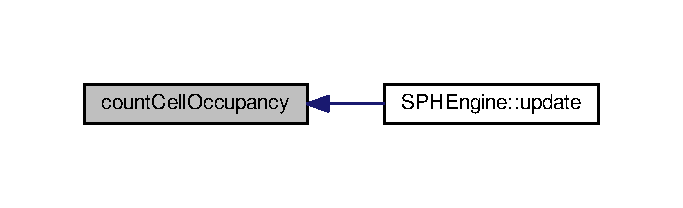
\includegraphics[width=328pt]{_cuda_s_p_h_kernals_8cu_a5f674fd3497767724a4425bbb91a2248_icgraph}
\end{center}
\end{figure}


\hypertarget{_cuda_s_p_h_kernals_8cu_a5ef63636297ac3ddbc0866064a75e12d}{\index{Cuda\-S\-P\-H\-Kernals.\-cu@{Cuda\-S\-P\-H\-Kernals.\-cu}!create\-Cell\-Idx@{create\-Cell\-Idx}}
\index{create\-Cell\-Idx@{create\-Cell\-Idx}!CudaSPHKernals.cu@{Cuda\-S\-P\-H\-Kernals.\-cu}}
\subsubsection[{create\-Cell\-Idx}]{\setlength{\rightskip}{0pt plus 5cm}void create\-Cell\-Idx (
\begin{DoxyParamCaption}
\item[{unsigned int $\ast$}]{d\-\_\-cell\-Occ\-Array, }
\item[{unsigned int}]{\-\_\-size, }
\item[{unsigned int $\ast$}]{d\-\_\-cell\-Idx\-Array}
\end{DoxyParamCaption}
)}}\label{_cuda_s_p_h_kernals_8cu_a5ef63636297ac3ddbc0866064a75e12d}


Creates an index array for our cells using thrusts exclusive scan. 


\begin{DoxyParams}{Parameters}
{\em d\-\_\-cell\-Occ\-Array} & -\/ pointer to our hash table cell occupancy buffer on our device \\
\hline
{\em \-\_\-size} & -\/ the size of our buffer on our divice \\
\hline
{\em d\-\_\-cell\-Idx\-Array} & -\/ our output buffer on our device to store our index's \\
\hline
\end{DoxyParams}


Here is the caller graph for this function\-:\nopagebreak
\begin{figure}[H]
\begin{center}
\leavevmode
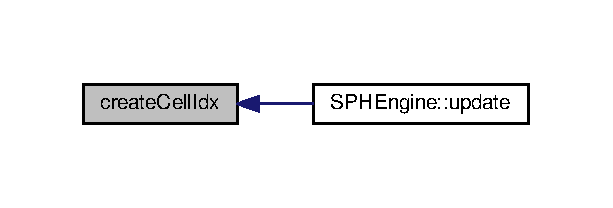
\includegraphics[width=294pt]{_cuda_s_p_h_kernals_8cu_a5ef63636297ac3ddbc0866064a75e12d_icgraph}
\end{center}
\end{figure}


\hypertarget{_cuda_s_p_h_kernals_8cu_afdcf7b761d59cb7dc7242693f8098380}{\index{Cuda\-S\-P\-H\-Kernals.\-cu@{Cuda\-S\-P\-H\-Kernals.\-cu}!create\-Hash\-Table@{create\-Hash\-Table}}
\index{create\-Hash\-Table@{create\-Hash\-Table}!CudaSPHKernals.cu@{Cuda\-S\-P\-H\-Kernals.\-cu}}
\subsubsection[{create\-Hash\-Table}]{\setlength{\rightskip}{0pt plus 5cm}void create\-Hash\-Table (
\begin{DoxyParamCaption}
\item[{cuda\-Stream\-\_\-t}]{\-\_\-stream, }
\item[{unsigned int $\ast$}]{d\-\_\-hash\-Array, }
\item[{float3 $\ast$}]{d\-\_\-pos\-Array, }
\item[{unsigned int}]{\-\_\-num\-Particles, }
\item[{float}]{\-\_\-smoothing\-Length, }
\item[{float}]{\-\_\-grid\-Size, }
\item[{int}]{\-\_\-max\-Num\-Threads}
\end{DoxyParamCaption}
)}}\label{_cuda_s_p_h_kernals_8cu_afdcf7b761d59cb7dc7242693f8098380}


Creates a spatial hash key based on our particle postion. 


\begin{DoxyParams}{Parameters}
{\em \-\_\-stream} & -\/ the cuda stream we wish this kernal to run on \\
\hline
{\em d\-\_\-hash\-Array} & -\/ a pointer to the cuda buffer that we wish to store our hash keys \\
\hline
{\em d\-\_\-pos\-Array} & -\/ pointer to the cuda buffer that holds the particle postions we wish to hash \\
\hline
{\em \-\_\-num\-Particles} & -\/ the number of particles. Used to calculate how many kernals to launch \\
\hline
{\em \-\_\-smoothing\-Length} & -\/ Smoothing length of our hash. How big each cell of our hash is. \\
\hline
{\em \-\_\-grid\-Size} & -\/ the size of our grid. .g. 1 is a grid of size 1$\ast$1$\ast$1. \\
\hline
{\em \-\_\-max\-Num\-Threads} & -\/ the maximum number off threads we have in a block on our device. Can be found out with device query \\
\hline
\end{DoxyParams}


Here is the caller graph for this function\-:\nopagebreak
\begin{figure}[H]
\begin{center}
\leavevmode
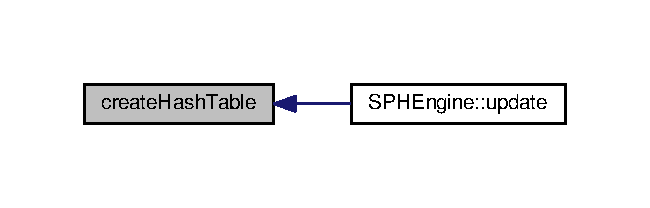
\includegraphics[width=312pt]{_cuda_s_p_h_kernals_8cu_afdcf7b761d59cb7dc7242693f8098380_icgraph}
\end{center}
\end{figure}


\hypertarget{_cuda_s_p_h_kernals_8cu_aaaee82afeb737d25fb86efb6949aa1b5}{\index{Cuda\-S\-P\-H\-Kernals.\-cu@{Cuda\-S\-P\-H\-Kernals.\-cu}!density\-Weighting@{density\-Weighting}}
\index{density\-Weighting@{density\-Weighting}!CudaSPHKernals.cu@{Cuda\-S\-P\-H\-Kernals.\-cu}}
\subsubsection[{density\-Weighting}]{\setlength{\rightskip}{0pt plus 5cm}\-\_\-\-\_\-device\-\_\-\-\_\- float density\-Weighting (
\begin{DoxyParamCaption}
\item[{float}]{\-\_\-dst, }
\item[{float}]{\-\_\-smoothing\-Length, }
\item[{float}]{\-\_\-dens\-Kern\-Const}
\end{DoxyParamCaption}
)}}\label{_cuda_s_p_h_kernals_8cu_aaaee82afeb737d25fb86efb6949aa1b5}


This is our desity weighting kernal used in our navier stokes equations. 


\begin{DoxyParams}{Parameters}
{\em \-\_\-dst} & -\/ the distance away of the neighbouring \\
\hline
{\em \-\_\-smoothing\-Length} & -\/ the smoothing length of our simulation. Can be thought of a hash cell size. \\
\hline
{\em \-\_\-dens\-Kern\-Cosnt} & -\/ constant part of our kernal. Easier to calculate once on C\-P\-U and have loaded into device kernal. \\
\hline
\end{DoxyParams}
\begin{DoxyReturn}{Returns}
return the weighting that our neighbouring particle has on our current particle 
\end{DoxyReturn}
\hypertarget{_cuda_s_p_h_kernals_8cu_a32490018a3312806721e0576ff6f8c7b}{\index{Cuda\-S\-P\-H\-Kernals.\-cu@{Cuda\-S\-P\-H\-Kernals.\-cu}!fill\-Uint@{fill\-Uint}}
\index{fill\-Uint@{fill\-Uint}!CudaSPHKernals.cu@{Cuda\-S\-P\-H\-Kernals.\-cu}}
\subsubsection[{fill\-Uint}]{\setlength{\rightskip}{0pt plus 5cm}void fill\-Uint (
\begin{DoxyParamCaption}
\item[{unsigned int $\ast$}]{\-\_\-pointer, }
\item[{unsigned int}]{\-\_\-array\-Size, }
\item[{unsigned int}]{\-\_\-fill}
\end{DoxyParamCaption}
)}}\label{_cuda_s_p_h_kernals_8cu_a32490018a3312806721e0576ff6f8c7b}


simple function so that we can fill a buffer with unsigned ints. 


\begin{DoxyParams}{Parameters}
{\em \-\_\-pointer} & -\/ pointer to the buffer you wish to fill \\
\hline
{\em \-\_\-array\-Size} & -\/ size of the buffer you wish to fill \\
\hline
{\em \-\_\-fill} & -\/ what you wish to fill it with \\
\hline
\end{DoxyParams}


Here is the caller graph for this function\-:\nopagebreak
\begin{figure}[H]
\begin{center}
\leavevmode
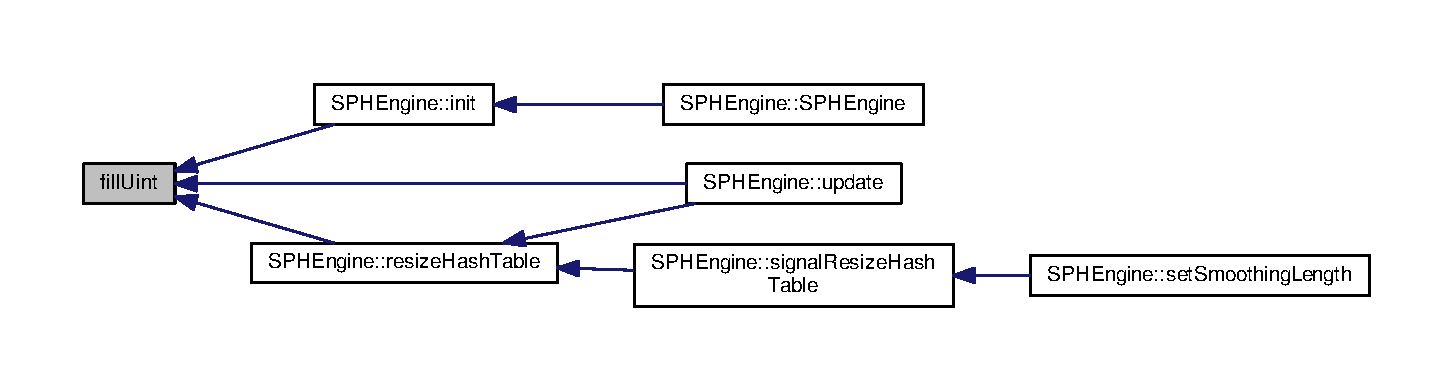
\includegraphics[width=350pt]{_cuda_s_p_h_kernals_8cu_a32490018a3312806721e0576ff6f8c7b_icgraph}
\end{center}
\end{figure}


\hypertarget{_cuda_s_p_h_kernals_8cu_a59c1e6aa2f1fb9792cde8f2ab4eba1d5}{\index{Cuda\-S\-P\-H\-Kernals.\-cu@{Cuda\-S\-P\-H\-Kernals.\-cu}!fluid\-Solver@{fluid\-Solver}}
\index{fluid\-Solver@{fluid\-Solver}!CudaSPHKernals.cu@{Cuda\-S\-P\-H\-Kernals.\-cu}}
\subsubsection[{fluid\-Solver}]{\setlength{\rightskip}{0pt plus 5cm}void fluid\-Solver (
\begin{DoxyParamCaption}
\item[{cuda\-Stream\-\_\-t}]{\-\_\-stream, }
\item[{float3 $\ast$}]{d\-\_\-pos\-Array, }
\item[{float3 $\ast$}]{d\-\_\-vel\-Array, }
\item[{unsigned int $\ast$}]{d\-\_\-cell\-Occ\-Array, }
\item[{unsigned int $\ast$}]{d\-\_\-cell\-Indx\-Array, }
\item[{unsigned int}]{\-\_\-hash\-Table\-Size, }
\item[{int}]{\-\_\-hash\-Resolution, }
\item[{unsigned int}]{\-\_\-max\-Num\-Threads, }
\item[{float}]{\-\_\-smoothing\-Length, }
\item[{float}]{\-\_\-timestep, }
\item[{float}]{\-\_\-particle\-Mass = {\ttfamily 1}, }
\item[{float}]{\-\_\-rest\-Density = {\ttfamily 1}, }
\item[{float}]{\-\_\-gas\-Constant = {\ttfamily 1}, }
\item[{float}]{\-\_\-vis\-Coef = {\ttfamily 1}, }
\item[{float}]{\-\_\-vel\-Correction = {\ttfamily 0.3}, }
\item[{float}]{\-\_\-dens\-Kern\-Const = {\ttfamily 1}, }
\item[{float}]{\-\_\-press\-Kern\-Const = {\ttfamily 1}, }
\item[{float}]{\-\_\-visc\-Kern\-Const = {\ttfamily 1}}
\end{DoxyParamCaption}
)}}\label{_cuda_s_p_h_kernals_8cu_a59c1e6aa2f1fb9792cde8f2ab4eba1d5}


Solver function that will call our solver kernal to calculate the new positions of the particles in. 

our fluid simulation. 
\begin{DoxyParams}{Parameters}
{\em \-\_\-stream} & -\/ the cuda stream we wish this kernal to run on \\
\hline
{\em d\-\_\-pos\-Array} & -\/ pointer to our gpu buffer that holds the postions of our particles \\
\hline
{\em d\-\_\-vel\-Array} & -\/ pointer to our gpu buffer that holds the velocities of our particles \\
\hline
{\em d\-\_\-cell\-Occ\-Array} & -\/ pointer to our gpu buffer that holds the cell occupancy count of our hash table \\
\hline
{\em d\-\_\-cell\-Indx\-Array} & -\/ pointer to our gpu buffer that holds the cell index's of our particles \\
\hline
{\em \-\_\-hash\-Table\-Size} & -\/ the size of our hash table. This is used to calculate how many blocks we need to launch our kernal with \\
\hline
{\em \-\_\-hash\-Resolution} & -\/ resolution of our hash table \\
\hline
{\em \-\_\-max\-Num\-Threads} & -\/ the maximum nuber of threads we need to launch per block \\
\hline
{\em \-\_\-smoothing\-Length} & -\/ smoothing length of our simulation. Can also be thought of as cell size. \\
\hline
{\em \-\_\-time\-Step} & -\/ the timestep that we want to increment our particles positions in our solver \\
\hline
{\em \-\_\-particle\-Mass} & -\/ the mass of each particle. Defaults to 1. \\
\hline
{\em \-\_\-rest\-Density} & -\/ the density of each particle at rest. Defaults to 1. \\
\hline
{\em \-\_\-gas\-Constant} & -\/ the gas constant of our fluid. Used for calculating pressure. Defaults to 1. \\
\hline
{\em \-\_\-vis\-Coef} & -\/ the coeficient of viscosity in our fluid simulation. Defaults to 1. \\
\hline
{\em \-\_\-vel\-Correction} & -\/ velocity correction using our X\-S\-P\-H method. Helps with compression, defaults to 0.\-3. \\
\hline
{\em \-\_\-dens\-Kern\-Const} & -\/ constant part of the density kernal. Faster to compute once on C\-P\-U and load in. \\
\hline
{\em \-\_\-press\-Kern\-Const} & -\/ constant part of the pressure kernal. Faster to compute once on C\-P\-U and load in. \\
\hline
{\em \-\_\-visc\-Kern\-Const} & -\/ constant part of the viscosity kernal. Faster to compute once on C\-P\-U and load in. \\
\hline
\end{DoxyParams}


Here is the caller graph for this function\-:\nopagebreak
\begin{figure}[H]
\begin{center}
\leavevmode
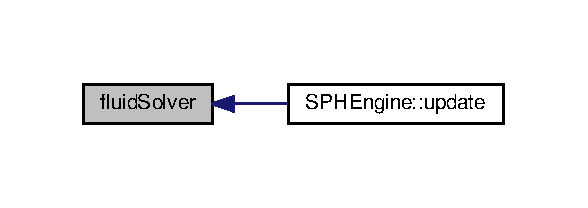
\includegraphics[width=282pt]{_cuda_s_p_h_kernals_8cu_a59c1e6aa2f1fb9792cde8f2ab4eba1d5_icgraph}
\end{center}
\end{figure}


\hypertarget{_cuda_s_p_h_kernals_8cu_afdcbd8ca539116cc7b8d030b1e418e77}{\index{Cuda\-S\-P\-H\-Kernals.\-cu@{Cuda\-S\-P\-H\-Kernals.\-cu}!point\-Hash@{point\-Hash}}
\index{point\-Hash@{point\-Hash}!CudaSPHKernals.cu@{Cuda\-S\-P\-H\-Kernals.\-cu}}
\subsubsection[{point\-Hash}]{\setlength{\rightskip}{0pt plus 5cm}\-\_\-\-\_\-global\-\_\-\-\_\- void point\-Hash (
\begin{DoxyParamCaption}
\item[{unsigned int $\ast$}]{d\-\_\-hash\-Array, }
\item[{float3 $\ast$}]{d\-\_\-pos\-Array, }
\item[{unsigned int}]{num\-Particles, }
\item[{float}]{resolution, }
\item[{float}]{\-\_\-grid\-Scaler}
\end{DoxyParamCaption}
)}}\label{_cuda_s_p_h_kernals_8cu_afdcbd8ca539116cc7b8d030b1e418e77}


Kernal designed to produce a has key based on the location of a particle. 

Hash function taken from Teschner, M., Heidelberger, B., Mueller, M., Pomeranets, D. and Gross, M. (2003). Optimized spatial hashing for collision detection of deformable objects 
\begin{DoxyParams}{Parameters}
{\em d\-\_\-hash\-Array} & -\/ pointer to a buffer to output our hash keys \\
\hline
{\em d\-\_\-pos\-Array} & -\/ pointer to the buffer that holds our particle positions \\
\hline
{\em num\-Particles} & -\/ the number of particles in our buffer \\
\hline
{\em resolution} & -\/ the resolution of our hash table \\
\hline
{\em \-\_\-grid\-Scaler} & -\/ Scales our points to between 0-\/1. \\
\hline
\end{DoxyParams}
\hypertarget{_cuda_s_p_h_kernals_8cu_ad44155cc5df4e6c30367f437d6fcb489}{\index{Cuda\-S\-P\-H\-Kernals.\-cu@{Cuda\-S\-P\-H\-Kernals.\-cu}!pressure\-Weighting@{pressure\-Weighting}}
\index{pressure\-Weighting@{pressure\-Weighting}!CudaSPHKernals.cu@{Cuda\-S\-P\-H\-Kernals.\-cu}}
\subsubsection[{pressure\-Weighting}]{\setlength{\rightskip}{0pt plus 5cm}\-\_\-\-\_\-device\-\_\-\-\_\- float3 pressure\-Weighting (
\begin{DoxyParamCaption}
\item[{float3}]{\-\_\-r, }
\item[{float}]{\-\_\-dst, }
\item[{float}]{\-\_\-smoothing\-Length, }
\item[{float}]{\-\_\-press\-Kern\-Const}
\end{DoxyParamCaption}
)}}\label{_cuda_s_p_h_kernals_8cu_ad44155cc5df4e6c30367f437d6fcb489}


This is our desity weighting kernal used in our navier stokes equations. 


\begin{DoxyParams}{Parameters}
{\em \-\_\-r} & -\/ vector from our neighbour particle to our current particle between 0$<$x$<$=smoothing\-Length \\
\hline
{\em \-\_\-dst} & -\/ the distance between our particles \\
\hline
{\em \-\_\-smoothing\-Length} & -\/ the smoothing length of our simulation. Can be thought of a hash cell size. \\
\hline
{\em \-\_\-press\-Kern\-Cosnt} & -\/ constant part of our kernal. Easier to calculate once on C\-P\-U and have loaded into device kernal. \\
\hline
\end{DoxyParams}
\begin{DoxyReturn}{Returns}
return the weighting that our neighbouring particle has on our current particle 
\end{DoxyReturn}
\hypertarget{_cuda_s_p_h_kernals_8cu_a1541f8b1ee73799a0cecc7030773a6a9}{\index{Cuda\-S\-P\-H\-Kernals.\-cu@{Cuda\-S\-P\-H\-Kernals.\-cu}!sort\-By\-Key@{sort\-By\-Key}}
\index{sort\-By\-Key@{sort\-By\-Key}!CudaSPHKernals.cu@{Cuda\-S\-P\-H\-Kernals.\-cu}}
\subsubsection[{sort\-By\-Key}]{\setlength{\rightskip}{0pt plus 5cm}void sort\-By\-Key (
\begin{DoxyParamCaption}
\item[{unsigned int $\ast$}]{d\-\_\-hash\-Array, }
\item[{float3 $\ast$}]{d\-\_\-pos\-Array, }
\item[{float3 $\ast$}]{d\-\_\-vel\-Array, }
\item[{unsigned int}]{\-\_\-num\-Particles}
\end{DoxyParamCaption}
)}}\label{_cuda_s_p_h_kernals_8cu_a1541f8b1ee73799a0cecc7030773a6a9}


Sorts our hash key buffer and postion buffer such that points of the same key occupy contiguous memory. 


\begin{DoxyParams}{Parameters}
{\em d\-\_\-hash\-Array} & -\/ pointer to our hash key buffer \\
\hline
{\em d\-\_\-pos\-Array} & -\/ pointer to our particle position buffer \\
\hline
{\em d\-\_\-vel\-Array} & -\/ pointer to our particle velocity buffer \\
\hline
{\em \-\_\-num\-Particles} & -\/ the number of particels in our buffer \\
\hline
\end{DoxyParams}


Here is the caller graph for this function\-:\nopagebreak
\begin{figure}[H]
\begin{center}
\leavevmode
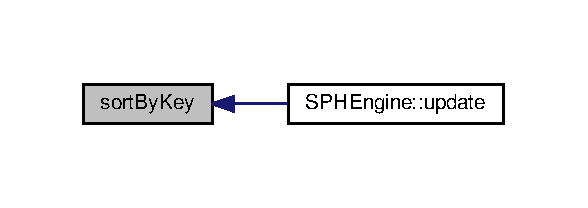
\includegraphics[width=282pt]{_cuda_s_p_h_kernals_8cu_a1541f8b1ee73799a0cecc7030773a6a9_icgraph}
\end{center}
\end{figure}


\hypertarget{_cuda_s_p_h_kernals_8cu_ad682f881cf72f537f3cad1ba7993b5b5}{\index{Cuda\-S\-P\-H\-Kernals.\-cu@{Cuda\-S\-P\-H\-Kernals.\-cu}!viscosity\-Weighting@{viscosity\-Weighting}}
\index{viscosity\-Weighting@{viscosity\-Weighting}!CudaSPHKernals.cu@{Cuda\-S\-P\-H\-Kernals.\-cu}}
\subsubsection[{viscosity\-Weighting}]{\setlength{\rightskip}{0pt plus 5cm}\-\_\-\-\_\-device\-\_\-\-\_\- float3 viscosity\-Weighting (
\begin{DoxyParamCaption}
\item[{float3}]{\-\_\-r, }
\item[{float}]{\-\_\-dst, }
\item[{float}]{\-\_\-smoothing\-Length, }
\item[{float}]{\-\_\-visc\-Kern\-Const}
\end{DoxyParamCaption}
)}}\label{_cuda_s_p_h_kernals_8cu_ad682f881cf72f537f3cad1ba7993b5b5}


This is our viscosty weighting kernal used in our navier stokes equations. 


\begin{DoxyParams}{Parameters}
{\em \-\_\-r} & -\/ vector from our neighbour particle to our current particle \\
\hline
{\em \-\_\-dst} & -\/ the distance between our particles \\
\hline
{\em \-\_\-smoothing\-Length} & -\/ the smoothing length of our simulation. Can be thought of a hash cell size. \\
\hline
{\em \-\_\-visc\-Kern\-Cosnt} & -\/ constant part of our kernal. Easier to calculate once on C\-P\-U and have loaded into device kernal. \\
\hline
\end{DoxyParams}
\begin{DoxyReturn}{Returns}
return the weighting that our neighbouring particle has on our current particle 
\end{DoxyReturn}

\hypertarget{_cuda_s_p_h_kernals_8h}{\section{include/\-Cuda\-S\-P\-H\-Kernals.h File Reference}
\label{_cuda_s_p_h_kernals_8h}\index{include/\-Cuda\-S\-P\-H\-Kernals.\-h@{include/\-Cuda\-S\-P\-H\-Kernals.\-h}}
}


Used for prototyping our our functions used for our S\-P\-H simulation calculations.  


{\ttfamily \#include $<$stdio.\-h$>$}\\*
\subsection*{Classes}
\begin{DoxyCompactItemize}
\item 
struct \hyperlink{structparticle_cell_prop}{particle\-Cell\-Prop}
\begin{DoxyCompactList}\small\item\em a structure to hold the properties of our particle cell \end{DoxyCompactList}\item 
struct \hyperlink{struct_simple_cuboid_collision_object}{Simple\-Cuboid\-Collision\-Object}
\begin{DoxyCompactList}\small\item\em a cuboid collion object properties \end{DoxyCompactList}\end{DoxyCompactItemize}
\subsection*{Functions}
\begin{DoxyCompactItemize}
\item 
void \hyperlink{_cuda_s_p_h_kernals_8h_a5ef63636297ac3ddbc0866064a75e12d}{create\-Cell\-Idx} (unsigned int $\ast$d\-\_\-cell\-Occ\-Array, unsigned int \-\_\-size, unsigned int $\ast$d\-\_\-cell\-Idx\-Array)
\begin{DoxyCompactList}\small\item\em Creates an index array for our cells using thrusts exclusive scan. \end{DoxyCompactList}\item 
void \hyperlink{_cuda_s_p_h_kernals_8h_afdcf7b761d59cb7dc7242693f8098380}{create\-Hash\-Table} (cuda\-Stream\-\_\-t \-\_\-stream, unsigned int $\ast$d\-\_\-hash\-Array, float3 $\ast$d\-\_\-pos\-Array, unsigned int \-\_\-num\-Particles, float \-\_\-smoothing\-Length, float \-\_\-grid\-Size, int \-\_\-max\-Num\-Threads)
\begin{DoxyCompactList}\small\item\em Creates a spatial hash key based on our particle postion. \end{DoxyCompactList}\item 
void \hyperlink{_cuda_s_p_h_kernals_8h_a1541f8b1ee73799a0cecc7030773a6a9}{sort\-By\-Key} (unsigned int $\ast$d\-\_\-hash\-Array, float3 $\ast$d\-\_\-pos\-Array, float3 $\ast$d\-\_\-vel\-Array, unsigned int \-\_\-num\-Particles)
\begin{DoxyCompactList}\small\item\em Sorts our hash key buffer and postion buffer such that points of the same key occupy contiguous memory. \end{DoxyCompactList}\item 
void \hyperlink{_cuda_s_p_h_kernals_8h_a5f674fd3497767724a4425bbb91a2248}{count\-Cell\-Occupancy} (cuda\-Stream\-\_\-t \-\_\-stream, unsigned int $\ast$d\-\_\-hash\-Array, unsigned int $\ast$d\-\_\-cell\-Occ\-Array, unsigned int \-\_\-hash\-Table\-Size, unsigned int \-\_\-num\-Points, unsigned int \-\_\-max\-Num\-Threads)
\begin{DoxyCompactList}\small\item\em Computes the particle occupancy of our hash cell. \end{DoxyCompactList}\item 
void \hyperlink{_cuda_s_p_h_kernals_8h_a32490018a3312806721e0576ff6f8c7b}{fill\-Uint} (unsigned int $\ast$\-\_\-pointer, unsigned int \-\_\-array\-Size, unsigned int \-\_\-fill)
\begin{DoxyCompactList}\small\item\em simple function so that we can fill a buffer with unsigned ints. \end{DoxyCompactList}\item 
void \hyperlink{_cuda_s_p_h_kernals_8h_adb6bcaa76e0b8b0bffe9b300e9579ade}{fluid\-Solver} (cuda\-Stream\-\_\-t \-\_\-stream, float3 $\ast$d\-\_\-pos\-Array, float3 $\ast$d\-\_\-vel\-Array, unsigned int $\ast$d\-\_\-cell\-Occ\-Array, unsigned int $\ast$d\-\_\-cell\-Indx\-Array, unsigned int \-\_\-hash\-Table\-Size, int \-\_\-hash\-Resolution, unsigned int \-\_\-max\-Num\-Threads, float \-\_\-smoothing\-Length, float \-\_\-timestep, float \-\_\-particle\-Mass=1, float \-\_\-rest\-Density=1, float \-\_\-gas\-Constant=1, float \-\_\-vis\-Coef=1, float \-\_\-vel\-Correction=0.\-3, float \-\_\-dens\-Kern\-Const=1, float \-\_\-press\-Kern\-Const=1, float \-\_\-visc\-Kern\-Const=1)
\begin{DoxyCompactList}\small\item\em Solver function that will call our solver kernal to calculate the new positions of the particles in. \end{DoxyCompactList}\item 
void \hyperlink{_cuda_s_p_h_kernals_8h_a1985239f9afd133a3db010848f3950f6}{collision\-Detection\-Solver} (cuda\-Stream\-\_\-t \-\_\-stream, \hyperlink{struct_simple_cuboid_collision_object}{Simple\-Cuboid\-Collision\-Object} $\ast$d\-\_\-plane\-Array, unsigned int \-\_\-num\-Objects, float3 $\ast$d\-\_\-pos\-Array, float3 $\ast$d\-\_\-vel\-Array, float \-\_\-time\-Step, unsigned int \-\_\-num\-Particles, unsigned int \-\_\-max\-Num\-Threads)
\begin{DoxyCompactList}\small\item\em Collision detection between particles and planes. \end{DoxyCompactList}\end{DoxyCompactItemize}


\subsection{Detailed Description}
Used for prototyping our our functions used for our S\-P\-H simulation calculations. \begin{DoxyAuthor}{Author}
Declan Russell 
\end{DoxyAuthor}
\begin{DoxyDate}{Date}
08/03/2015 
\end{DoxyDate}
\begin{DoxyVersion}{Version}
1.\-0 This file is linked with \hyperlink{_cuda_s_p_h_kernals_8cu}{Cuda\-S\-P\-H\-Kernals.\-cu} by gcc after \hyperlink{_cuda_s_p_h_kernals_8cu}{Cuda\-S\-P\-H\-Kernals.\-cu} has been compiled by nvcc. 
\end{DoxyVersion}


\subsection{Function Documentation}
\hypertarget{_cuda_s_p_h_kernals_8h_a1985239f9afd133a3db010848f3950f6}{\index{Cuda\-S\-P\-H\-Kernals.\-h@{Cuda\-S\-P\-H\-Kernals.\-h}!collision\-Detection\-Solver@{collision\-Detection\-Solver}}
\index{collision\-Detection\-Solver@{collision\-Detection\-Solver}!CudaSPHKernals.h@{Cuda\-S\-P\-H\-Kernals.\-h}}
\subsubsection[{collision\-Detection\-Solver}]{\setlength{\rightskip}{0pt plus 5cm}void collision\-Detection\-Solver (
\begin{DoxyParamCaption}
\item[{cuda\-Stream\-\_\-t}]{\-\_\-stream, }
\item[{{\bf Simple\-Cuboid\-Collision\-Object} $\ast$}]{d\-\_\-plane\-Array, }
\item[{unsigned int}]{\-\_\-num\-Objects, }
\item[{float3 $\ast$}]{d\-\_\-pos\-Array, }
\item[{float3 $\ast$}]{d\-\_\-vel\-Array, }
\item[{float}]{\-\_\-time\-Step, }
\item[{unsigned int}]{\-\_\-num\-Particles, }
\item[{unsigned int}]{\-\_\-max\-Num\-Threads}
\end{DoxyParamCaption}
)}}\label{_cuda_s_p_h_kernals_8h_a1985239f9afd133a3db010848f3950f6}


Collision detection between particles and planes. 


\begin{DoxyParams}{Parameters}
{\em \-\_\-stream} & -\/ the cuda stream we wish this kernal to run on \\
\hline
{\em d\-\_\-\-Plane\-Array} & -\/ pointer to device buffer of our planes information \\
\hline
{\em \-\_\-num\-Planes} & -\/ number of planes in our array \\
\hline
{\em d\-\_\-pos\-Array} & -\/ pointer to device buffer of our particle positions \\
\hline
{\em d\-\_\-vel\-Array} & -\/ pointer to device buffer of our particle velocities \\
\hline
{\em \-\_\-time\-Step} & -\/ time step of our update \\
\hline
{\em \-\_\-num\-Particles} & -\/ the number of particles in our scene \\
\hline
{\em \-\_\-max\-Num\-Threads} & -\/ the maximum nuber of threads we need to launch per block \\
\hline
\end{DoxyParams}
\hypertarget{_cuda_s_p_h_kernals_8h_a5f674fd3497767724a4425bbb91a2248}{\index{Cuda\-S\-P\-H\-Kernals.\-h@{Cuda\-S\-P\-H\-Kernals.\-h}!count\-Cell\-Occupancy@{count\-Cell\-Occupancy}}
\index{count\-Cell\-Occupancy@{count\-Cell\-Occupancy}!CudaSPHKernals.h@{Cuda\-S\-P\-H\-Kernals.\-h}}
\subsubsection[{count\-Cell\-Occupancy}]{\setlength{\rightskip}{0pt plus 5cm}void count\-Cell\-Occupancy (
\begin{DoxyParamCaption}
\item[{cuda\-Stream\-\_\-t}]{\-\_\-stream, }
\item[{unsigned int $\ast$}]{d\-\_\-hash\-Array, }
\item[{unsigned int $\ast$}]{d\-\_\-cell\-Occ\-Array, }
\item[{unsigned int}]{\-\_\-hash\-Table\-Size, }
\item[{unsigned int}]{\-\_\-num\-Points, }
\item[{unsigned int}]{\-\_\-max\-Num\-Threads}
\end{DoxyParamCaption}
)}}\label{_cuda_s_p_h_kernals_8h_a5f674fd3497767724a4425bbb91a2248}


Computes the particle occupancy of our hash cell. 


\begin{DoxyParams}{Parameters}
{\em \-\_\-stream} & -\/ the cuda stream we wish this kernal to run on \\
\hline
{\em d\-\_\-hash\-Array} & -\/ pointer to our hash key buffer \\
\hline
{\em d\-\_\-cell\-Occ\-Array} & -\/ pointer to our cell occupancy array \\
\hline
{\em \-\_\-hash\-Table\-Size} & -\/ size of our hash table \\
\hline
{\em \-\_\-num\-Points} & -\/ number of points in our hash table \\
\hline
{\em \-\_\-max\-Num\-Threads} & -\/ the maximum number of threads that we have per block on our device \\
\hline
\end{DoxyParams}
\hypertarget{_cuda_s_p_h_kernals_8h_a5ef63636297ac3ddbc0866064a75e12d}{\index{Cuda\-S\-P\-H\-Kernals.\-h@{Cuda\-S\-P\-H\-Kernals.\-h}!create\-Cell\-Idx@{create\-Cell\-Idx}}
\index{create\-Cell\-Idx@{create\-Cell\-Idx}!CudaSPHKernals.h@{Cuda\-S\-P\-H\-Kernals.\-h}}
\subsubsection[{create\-Cell\-Idx}]{\setlength{\rightskip}{0pt plus 5cm}void create\-Cell\-Idx (
\begin{DoxyParamCaption}
\item[{unsigned int $\ast$}]{d\-\_\-cell\-Occ\-Array, }
\item[{unsigned int}]{\-\_\-size, }
\item[{unsigned int $\ast$}]{d\-\_\-cell\-Idx\-Array}
\end{DoxyParamCaption}
)}}\label{_cuda_s_p_h_kernals_8h_a5ef63636297ac3ddbc0866064a75e12d}


Creates an index array for our cells using thrusts exclusive scan. 


\begin{DoxyParams}{Parameters}
{\em d\-\_\-cell\-Occ\-Array} & -\/ pointer to our hash table cell occupancy buffer on our device \\
\hline
{\em \-\_\-size} & -\/ the size of our buffer on our divice \\
\hline
{\em d\-\_\-cell\-Idx\-Array} & -\/ our output buffer on our device to store our index's \\
\hline
\end{DoxyParams}
\hypertarget{_cuda_s_p_h_kernals_8h_afdcf7b761d59cb7dc7242693f8098380}{\index{Cuda\-S\-P\-H\-Kernals.\-h@{Cuda\-S\-P\-H\-Kernals.\-h}!create\-Hash\-Table@{create\-Hash\-Table}}
\index{create\-Hash\-Table@{create\-Hash\-Table}!CudaSPHKernals.h@{Cuda\-S\-P\-H\-Kernals.\-h}}
\subsubsection[{create\-Hash\-Table}]{\setlength{\rightskip}{0pt plus 5cm}void create\-Hash\-Table (
\begin{DoxyParamCaption}
\item[{cuda\-Stream\-\_\-t}]{\-\_\-stream, }
\item[{unsigned int $\ast$}]{d\-\_\-hash\-Array, }
\item[{float3 $\ast$}]{d\-\_\-pos\-Array, }
\item[{unsigned int}]{\-\_\-num\-Particles, }
\item[{float}]{\-\_\-smoothing\-Length, }
\item[{float}]{\-\_\-grid\-Size, }
\item[{int}]{\-\_\-max\-Num\-Threads}
\end{DoxyParamCaption}
)}}\label{_cuda_s_p_h_kernals_8h_afdcf7b761d59cb7dc7242693f8098380}


Creates a spatial hash key based on our particle postion. 

This is taken from Teschner, M., Heidelberger, B., Mueller, M., Pomeranets, D. and Gross, M. (2003). Optimized spatial hashing for collision detection of deformable objects 
\begin{DoxyParams}{Parameters}
{\em \-\_\-stream} & -\/ the cuda stream we wish this kernal to run on \\
\hline
{\em d\-\_\-hash\-Array} & -\/ a pointer to the cuda buffer that we wish to store our hash keys \\
\hline
{\em d\-\_\-pos\-Array} & -\/ pointer to the cuda buffer that holds the particle postions we wish to hash \\
\hline
{\em \-\_\-num\-Particles} & -\/ the number of particles. Used to calculate how many kernals to launch \\
\hline
{\em \-\_\-smoothing\-Length} & -\/ Smoothing length of our hash. How big each cell of our hash is. \\
\hline
{\em \-\_\-grid\-Size} & -\/ the size of our grid. .g. 1 is a grid of size 1$\ast$1$\ast$1. \\
\hline
{\em \-\_\-max\-Num\-Threads} & -\/ the maximum number off threads we have in a block on our device. Can be found out with device query \\
\hline
\end{DoxyParams}
\hypertarget{_cuda_s_p_h_kernals_8h_a32490018a3312806721e0576ff6f8c7b}{\index{Cuda\-S\-P\-H\-Kernals.\-h@{Cuda\-S\-P\-H\-Kernals.\-h}!fill\-Uint@{fill\-Uint}}
\index{fill\-Uint@{fill\-Uint}!CudaSPHKernals.h@{Cuda\-S\-P\-H\-Kernals.\-h}}
\subsubsection[{fill\-Uint}]{\setlength{\rightskip}{0pt plus 5cm}void fill\-Uint (
\begin{DoxyParamCaption}
\item[{unsigned int $\ast$}]{\-\_\-pointer, }
\item[{unsigned int}]{\-\_\-array\-Size, }
\item[{unsigned int}]{\-\_\-fill}
\end{DoxyParamCaption}
)}}\label{_cuda_s_p_h_kernals_8h_a32490018a3312806721e0576ff6f8c7b}


simple function so that we can fill a buffer with unsigned ints. 


\begin{DoxyParams}{Parameters}
{\em \-\_\-pointer} & -\/ pointer to the buffer you wish to fill \\
\hline
{\em \-\_\-array\-Size} & -\/ size of the buffer you wish to fill \\
\hline
{\em \-\_\-fill} & -\/ what you wish to fill it with \\
\hline
\end{DoxyParams}
\hypertarget{_cuda_s_p_h_kernals_8h_adb6bcaa76e0b8b0bffe9b300e9579ade}{\index{Cuda\-S\-P\-H\-Kernals.\-h@{Cuda\-S\-P\-H\-Kernals.\-h}!fluid\-Solver@{fluid\-Solver}}
\index{fluid\-Solver@{fluid\-Solver}!CudaSPHKernals.h@{Cuda\-S\-P\-H\-Kernals.\-h}}
\subsubsection[{fluid\-Solver}]{\setlength{\rightskip}{0pt plus 5cm}void fluid\-Solver (
\begin{DoxyParamCaption}
\item[{cuda\-Stream\-\_\-t}]{\-\_\-stream, }
\item[{float3 $\ast$}]{d\-\_\-pos\-Array, }
\item[{float3 $\ast$}]{d\-\_\-vel\-Array, }
\item[{unsigned int $\ast$}]{d\-\_\-cell\-Occ\-Array, }
\item[{unsigned int $\ast$}]{d\-\_\-cell\-Indx\-Array, }
\item[{unsigned int}]{\-\_\-hash\-Table\-Size, }
\item[{int}]{\-\_\-hash\-Resolution, }
\item[{unsigned int}]{\-\_\-max\-Num\-Threads, }
\item[{float}]{\-\_\-smoothing\-Length, }
\item[{float}]{\-\_\-timestep, }
\item[{float}]{\-\_\-particle\-Mass = {\ttfamily 1}, }
\item[{float}]{\-\_\-rest\-Density = {\ttfamily 1}, }
\item[{float}]{\-\_\-gas\-Constant = {\ttfamily 1}, }
\item[{float}]{\-\_\-vis\-Coef = {\ttfamily 1}, }
\item[{float}]{\-\_\-vel\-Correction = {\ttfamily 0.3}, }
\item[{float}]{\-\_\-dens\-Kern\-Const = {\ttfamily 1}, }
\item[{float}]{\-\_\-press\-Kern\-Const = {\ttfamily 1}, }
\item[{float}]{\-\_\-visc\-Kern\-Const = {\ttfamily 1}}
\end{DoxyParamCaption}
)}}\label{_cuda_s_p_h_kernals_8h_adb6bcaa76e0b8b0bffe9b300e9579ade}


Solver function that will call our solver kernal to calculate the new positions of the particles in. 

our fluid simulation. 
\begin{DoxyParams}{Parameters}
{\em \-\_\-stream} & -\/ the cuda stream we wish this kernal to run on \\
\hline
{\em d\-\_\-pos\-Array} & -\/ pointer to our gpu buffer that holds the postions of our particles \\
\hline
{\em d\-\_\-vel\-Array} & -\/ pointer to our gpu buffer that holds the velocities of our particles \\
\hline
{\em d\-\_\-acc\-Array} & -\/ pointer to our gpu buffer that holds the accelleration of our particles \\
\hline
{\em d\-\_\-cell\-Occ\-Array} & -\/ pointer to our gpu buffer that holds the cell occupancy count of our hash table \\
\hline
{\em d\-\_\-cell\-Indx\-Array} & -\/ pointer to our gpu buffer that holds the cell index's of our particles \\
\hline
{\em \-\_\-hash\-Table\-Size} & -\/ the size of our hash table. This is used to calculate how many blocks we need to launch our kernal with \\
\hline
{\em \-\_\-max\-Num\-Threads} & -\/ the maximum nuber of threads we need to launch per block \\
\hline
{\em \-\_\-smoothing\-Length} & -\/ smoothing length of our simulation. Can also be thought of as cell size. \\
\hline
{\em \-\_\-time\-Step} & -\/ the timestep that we want to increment our particles positions in our solver \\
\hline
{\em \-\_\-particle\-Mass} & -\/ the mass of each particle. Defaults to 1. \\
\hline
{\em \-\_\-rest\-Density} & -\/ the density of each particle at rest. Defaults to 1. \\
\hline
{\em \-\_\-gas\-Constant} & -\/ the gas constant of our fluid. Used for calculating pressure. Defaults to 1. \\
\hline
{\em \-\_\-vis\-Coef} & -\/ the coeficient of viscosity in our fluid simulation. Defaults to 1. \\
\hline
{\em \-\_\-vel\-Correction} & -\/ velocity correction using our X\-S\-P\-H method. Helps with compression, defaults to 0.\-3. \\
\hline
{\em \-\_\-dens\-Kern\-Const} & -\/ constant part of the density kernal. Faster to compute once on C\-P\-U and load in. \\
\hline
{\em \-\_\-press\-Kern\-Const} & -\/ constant part of the pressure kernal. Faster to compute once on C\-P\-U and load in. \\
\hline
{\em \-\_\-visc\-Kern\-Const} & -\/ constant part of the viscosity kernal. Faster to compute once on C\-P\-U and load in. \\
\hline
\end{DoxyParams}
\hypertarget{_cuda_s_p_h_kernals_8h_a1541f8b1ee73799a0cecc7030773a6a9}{\index{Cuda\-S\-P\-H\-Kernals.\-h@{Cuda\-S\-P\-H\-Kernals.\-h}!sort\-By\-Key@{sort\-By\-Key}}
\index{sort\-By\-Key@{sort\-By\-Key}!CudaSPHKernals.h@{Cuda\-S\-P\-H\-Kernals.\-h}}
\subsubsection[{sort\-By\-Key}]{\setlength{\rightskip}{0pt plus 5cm}void sort\-By\-Key (
\begin{DoxyParamCaption}
\item[{unsigned int $\ast$}]{d\-\_\-hash\-Array, }
\item[{float3 $\ast$}]{d\-\_\-pos\-Array, }
\item[{float3 $\ast$}]{d\-\_\-vel\-Array, }
\item[{unsigned int}]{\-\_\-num\-Particles}
\end{DoxyParamCaption}
)}}\label{_cuda_s_p_h_kernals_8h_a1541f8b1ee73799a0cecc7030773a6a9}


Sorts our hash key buffer and postion buffer such that points of the same key occupy contiguous memory. 


\begin{DoxyParams}{Parameters}
{\em d\-\_\-hash\-Array} & -\/ pointer to our hash key buffer \\
\hline
{\em d\-\_\-pos\-Array} & -\/ pointer to our particle position buffer \\
\hline
{\em d\-\_\-vel\-Array} & -\/ pointer to our particle velocity buffer \\
\hline
{\em d\-\_\-acc\-Array} & -\/ pointer to our particle acceleration buffer \\
\hline
{\em \-\_\-num\-Particles} & -\/ the number of particels in our buffer \\
\hline
\end{DoxyParams}

\hypertarget{_open_g_l_widget_8h}{\section{include/\-Open\-G\-L\-Widget.h File Reference}
\label{_open_g_l_widget_8h}\index{include/\-Open\-G\-L\-Widget.\-h@{include/\-Open\-G\-L\-Widget.\-h}}
}
{\ttfamily \#include $<$G\-L/glew.\-h$>$}\\*
{\ttfamily \#include $<$Q\-G\-L\-Widget$>$}\\*
{\ttfamily \#include $<$Q\-Event$>$}\\*
{\ttfamily \#include $<$Q\-Resize\-Event$>$}\\*
{\ttfamily \#include $<$Q\-Message\-Box$>$}\\*
{\ttfamily \#include $<$Q\-String$>$}\\*
{\ttfamily \#include $<$Q\-Time$>$}\\*
{\ttfamily \#include $<$Q\-Color$>$}\\*
{\ttfamily \#include $<$ngl/\-Mat4.\-h$>$}\\*
{\ttfamily \#include $<$ngl/\-Camera.\-h$>$}\\*
{\ttfamily \#include $<$ngl/\-Text.\-h$>$}\\*
{\ttfamily \#include \char`\"{}S\-P\-H\-Engine.\-h\char`\"{}}\\*
{\ttfamily \#include \char`\"{}Fluid\-Shader.\-h\char`\"{}}\\*
\subsection*{Classes}
\begin{DoxyCompactItemize}
\item 
class \hyperlink{class_open_g_l_widget}{Open\-G\-L\-Widget}
\begin{DoxyCompactList}\small\item\em Basic Qt widget that holds a Open\-G\-L context. \end{DoxyCompactList}\end{DoxyCompactItemize}

\hypertarget{_s_p_h_engine_8h}{\section{include/\-S\-P\-H\-Engine.h File Reference}
\label{_s_p_h_engine_8h}\index{include/\-S\-P\-H\-Engine.\-h@{include/\-S\-P\-H\-Engine.\-h}}
}
{\ttfamily \#include $<$G\-L/glew.\-h$>$}\\*
{\ttfamily \#include $<$cuda\-\_\-runtime.\-h$>$}\\*
{\ttfamily \#include $<$cuda\-\_\-gl\-\_\-interop.\-h$>$}\\*
{\ttfamily \#include \char`\"{}Cuda\-S\-P\-H\-Kernals.\-h\char`\"{}}\\*
\subsection*{Classes}
\begin{DoxyCompactItemize}
\item 
class \hyperlink{class_s_p_h_engine}{S\-P\-H\-Engine}
\begin{DoxyCompactList}\small\item\em our cuda libraries \end{DoxyCompactList}\end{DoxyCompactItemize}

\hypertarget{bilateral_filter_frag_8glsl}{\section{/home/dexternation/\-A\-G\-S\-D\-T\-Fluid\-Sim/shaders/bilateral\-Filter\-Frag.glsl File Reference}
\label{bilateral_filter_frag_8glsl}\index{/home/dexternation/\-A\-G\-S\-D\-T\-Fluid\-Sim/shaders/bilateral\-Filter\-Frag.\-glsl@{/home/dexternation/\-A\-G\-S\-D\-T\-Fluid\-Sim/shaders/bilateral\-Filter\-Frag.\-glsl}}
}
\subsection*{Functions}
\begin{DoxyCompactItemize}
\item 
float \hyperlink{bilateral_filter_frag_8glsl_a4a4466509a3efe0b0eb00be16e5da684}{bil\-Filter} (vec2 blur\-Dir, float depth)
\begin{DoxyCompactList}\small\item\em our bilateral filter function \end{DoxyCompactList}\item 
\hypertarget{bilateral_filter_frag_8glsl_a6288eba0f8e8ad3ab1544ad731eb7667}{void \hyperlink{bilateral_filter_frag_8glsl_a6288eba0f8e8ad3ab1544ad731eb7667}{main} (void)}\label{bilateral_filter_frag_8glsl_a6288eba0f8e8ad3ab1544ad731eb7667}

\begin{DoxyCompactList}\small\item\em our main shader function \end{DoxyCompactList}\end{DoxyCompactItemize}
\subsection*{Variables}
\begin{DoxyCompactItemize}
\item 
\hypertarget{bilateral_filter_frag_8glsl_a3b19027caa70314998e90a0e13d915d3}{in vec2 \hyperlink{bilateral_filter_frag_8glsl_a3b19027caa70314998e90a0e13d915d3}{V\-Tex\-Coord}}\label{bilateral_filter_frag_8glsl_a3b19027caa70314998e90a0e13d915d3}

\begin{DoxyCompactList}\small\item\em in variable of the texture coordinates \end{DoxyCompactList}\item 
\hypertarget{bilateral_filter_frag_8glsl_ab59292ab7df136fb38e0290755f90dea}{uniform sampler2\-D \hyperlink{bilateral_filter_frag_8glsl_ab59292ab7df136fb38e0290755f90dea}{depth\-Tex}}\label{bilateral_filter_frag_8glsl_ab59292ab7df136fb38e0290755f90dea}

\begin{DoxyCompactList}\small\item\em texture for holding the depth pass \end{DoxyCompactList}\item 
\hypertarget{bilateral_filter_frag_8glsl_a834f840f0604abea8d2500555d4fb854}{uniform float \hyperlink{bilateral_filter_frag_8glsl_a834f840f0604abea8d2500555d4fb854}{blur\-Depth\-Falloff}}\label{bilateral_filter_frag_8glsl_a834f840f0604abea8d2500555d4fb854}

\begin{DoxyCompactList}\small\item\em unifrom to set the blur falloff \end{DoxyCompactList}\item 
\hypertarget{bilateral_filter_frag_8glsl_a2d45ac1478cca0b31f3b65fff9cb3530}{uniform float \hyperlink{bilateral_filter_frag_8glsl_a2d45ac1478cca0b31f3b65fff9cb3530}{filter\-Radius}}\label{bilateral_filter_frag_8glsl_a2d45ac1478cca0b31f3b65fff9cb3530}

\begin{DoxyCompactList}\small\item\em uniform to set the blur radius \end{DoxyCompactList}\item 
\hypertarget{bilateral_filter_frag_8glsl_a8a381e990c0bb33ed6cf2e9f97faf0d9}{uniform float \hyperlink{bilateral_filter_frag_8glsl_a8a381e990c0bb33ed6cf2e9f97faf0d9}{texel\-Size}}\label{bilateral_filter_frag_8glsl_a8a381e990c0bb33ed6cf2e9f97faf0d9}

\begin{DoxyCompactList}\small\item\em uniform for the size of our texel \end{DoxyCompactList}\item 
\hypertarget{bilateral_filter_frag_8glsl_a575f888600764d6ebd67a3fd89a7d034}{out vec4 \hyperlink{bilateral_filter_frag_8glsl_a575f888600764d6ebd67a3fd89a7d034}{fragout}}\label{bilateral_filter_frag_8glsl_a575f888600764d6ebd67a3fd89a7d034}

\begin{DoxyCompactList}\small\item\em our out our fragment \end{DoxyCompactList}\end{DoxyCompactItemize}


\subsection{Detailed Description}
\begin{DoxyAuthor}{Author}
Declan Russell 
\end{DoxyAuthor}
\begin{DoxyDate}{Date}
14/03/15 
\end{DoxyDate}
\begin{DoxyVersion}{Version}
2.\-0  G\-L\-S\-L 
\end{DoxyVersion}


\subsection{Function Documentation}
\hypertarget{bilateral_filter_frag_8glsl_a4a4466509a3efe0b0eb00be16e5da684}{\index{bilateral\-Filter\-Frag.\-glsl@{bilateral\-Filter\-Frag.\-glsl}!bil\-Filter@{bil\-Filter}}
\index{bil\-Filter@{bil\-Filter}!bilateralFilterFrag.glsl@{bilateral\-Filter\-Frag.\-glsl}}
\subsubsection[{bil\-Filter}]{\setlength{\rightskip}{0pt plus 5cm}float bil\-Filter (
\begin{DoxyParamCaption}
\item[{vec2}]{blur\-Dir, }
\item[{float}]{depth}
\end{DoxyParamCaption}
)}}\label{bilateral_filter_frag_8glsl_a4a4466509a3efe0b0eb00be16e5da684}


our bilateral filter function 


\begin{DoxyParams}{Parameters}
{\em blur\-Dir} & -\/ the direction of our blur \\
\hline
{\em depth} & -\/ the depth of our current input fragment \\
\hline
\end{DoxyParams}


Here is the caller graph for this function\-:\nopagebreak
\begin{figure}[H]
\begin{center}
\leavevmode
\includegraphics[width=202pt]{bilateral_filter_frag_8glsl_a4a4466509a3efe0b0eb00be16e5da684_icgraph}
\end{center}
\end{figure}



\hypertarget{bilateral_filter_vert_8glsl}{\section{shaders/bilateral\-Filter\-Vert.glsl File Reference}
\label{bilateral_filter_vert_8glsl}\index{shaders/bilateral\-Filter\-Vert.\-glsl@{shaders/bilateral\-Filter\-Vert.\-glsl}}
}
\subsection*{Functions}
\begin{DoxyCompactItemize}
\item 
\hyperlink{bilateral_filter_vert_8glsl_a76e82f4a2abee8cef9ec3419ca1ad185}{layout} (location=0) in vec2 vertex\-Position
\begin{DoxyCompactList}\small\item\em our vertex postion buffer \end{DoxyCompactList}\item 
\hypertarget{bilateral_filter_vert_8glsl_a6288eba0f8e8ad3ab1544ad731eb7667}{void \hyperlink{bilateral_filter_vert_8glsl_a6288eba0f8e8ad3ab1544ad731eb7667}{main} (void)}\label{bilateral_filter_vert_8glsl_a6288eba0f8e8ad3ab1544ad731eb7667}

\begin{DoxyCompactList}\small\item\em our main vertex function \end{DoxyCompactList}\end{DoxyCompactItemize}
\subsection*{Variables}
\begin{DoxyCompactItemize}
\item 
\hypertarget{bilateral_filter_vert_8glsl_a849580e4568e3dc8125d8e541b50a483}{out vec2 \hyperlink{bilateral_filter_vert_8glsl_a849580e4568e3dc8125d8e541b50a483}{V\-Tex\-Coord}}\label{bilateral_filter_vert_8glsl_a849580e4568e3dc8125d8e541b50a483}

\begin{DoxyCompactList}\small\item\em tex\-Coords to be passed to our fragment shader \end{DoxyCompactList}\end{DoxyCompactItemize}


\subsection{Detailed Description}
\begin{DoxyAuthor}{Author}
Declan Russell 
\end{DoxyAuthor}
\begin{DoxyDate}{Date}
14/03/15 
\end{DoxyDate}
\begin{DoxyVersion}{Version}
1.\-0  G\-L\-S\-L 
\end{DoxyVersion}


\subsection{Function Documentation}
\hypertarget{bilateral_filter_vert_8glsl_a76e82f4a2abee8cef9ec3419ca1ad185}{\index{bilateral\-Filter\-Vert.\-glsl@{bilateral\-Filter\-Vert.\-glsl}!layout@{layout}}
\index{layout@{layout}!bilateralFilterVert.glsl@{bilateral\-Filter\-Vert.\-glsl}}
\subsubsection[{layout}]{\setlength{\rightskip}{0pt plus 5cm}layout (
\begin{DoxyParamCaption}
\item[{location}]{ = {\ttfamily 0}}
\end{DoxyParamCaption}
)}}\label{bilateral_filter_vert_8glsl_a76e82f4a2abee8cef9ec3419ca1ad185}


our vertex postion buffer 

our vertex texcoord buffer 
\hypertarget{fluid_shader_frag_8glsl}{\section{shaders/fluid\-Shader\-Frag.glsl File Reference}
\label{fluid_shader_frag_8glsl}\index{shaders/fluid\-Shader\-Frag.\-glsl@{shaders/fluid\-Shader\-Frag.\-glsl}}
}
\subsection*{Classes}
\begin{DoxyCompactItemize}
\item 
struct \hyperlink{structlight_info}{light\-Info}
\begin{DoxyCompactList}\small\item\em a structure to hold our light information \end{DoxyCompactList}\end{DoxyCompactItemize}
\subsection*{Functions}
\begin{DoxyCompactItemize}
\item 
vec3 \hyperlink{fluid_shader_frag_8glsl_aa92a70677efb9df36d42919ab01aaaf4}{ads} (vec3 \hyperlink{thickness_vert_8glsl_af78042b263da1185c97c3202ced45aab}{position}, vec3 normal)
\begin{DoxyCompactList}\small\item\em calculates our phong shading \end{DoxyCompactList}\item 
vec3 \hyperlink{fluid_shader_frag_8glsl_abd810f8b2d0a0892c1c9d96228c3017d}{uv\-To\-Eye} (vec2 \-\_\-uv, float \-\_\-depth)
\begin{DoxyCompactList}\small\item\em converts uv coords and depth to eye space coodinates \end{DoxyCompactList}\item 
\hypertarget{fluid_shader_frag_8glsl_a6288eba0f8e8ad3ab1544ad731eb7667}{void \hyperlink{fluid_shader_frag_8glsl_a6288eba0f8e8ad3ab1544ad731eb7667}{main} (void)}\label{fluid_shader_frag_8glsl_a6288eba0f8e8ad3ab1544ad731eb7667}

\begin{DoxyCompactList}\small\item\em our fragment shader main \end{DoxyCompactList}\end{DoxyCompactItemize}
\subsection*{Variables}
\begin{DoxyCompactItemize}
\item 
\hypertarget{fluid_shader_frag_8glsl_ab59292ab7df136fb38e0290755f90dea}{uniform sampler2\-D \hyperlink{fluid_shader_frag_8glsl_ab59292ab7df136fb38e0290755f90dea}{depth\-Tex}}\label{fluid_shader_frag_8glsl_ab59292ab7df136fb38e0290755f90dea}

\begin{DoxyCompactList}\small\item\em texture for holding the depth pass \end{DoxyCompactList}\item 
\hypertarget{fluid_shader_frag_8glsl_ae98cad87e3271b9fe544fdeb6cb0ec5a}{uniform sampler2\-D \hyperlink{fluid_shader_frag_8glsl_ae98cad87e3271b9fe544fdeb6cb0ec5a}{thickness\-Tex}}\label{fluid_shader_frag_8glsl_ae98cad87e3271b9fe544fdeb6cb0ec5a}

\begin{DoxyCompactList}\small\item\em texture for holding the thickness pass \end{DoxyCompactList}\item 
\hypertarget{fluid_shader_frag_8glsl_a9dac566b8dcb58f380dec54a9a51b3fa}{uniform sampler\-Cube \hyperlink{fluid_shader_frag_8glsl_a9dac566b8dcb58f380dec54a9a51b3fa}{cube\-Map\-Tex}}\label{fluid_shader_frag_8glsl_a9dac566b8dcb58f380dec54a9a51b3fa}

\begin{DoxyCompactList}\small\item\em texture for holding the cube map \end{DoxyCompactList}\item 
\hypertarget{fluid_shader_frag_8glsl_a2e4c2975a979371b6b81bc6c96378ec4}{uniform float \hyperlink{fluid_shader_frag_8glsl_a2e4c2975a979371b6b81bc6c96378ec4}{texel\-Size\-X}}\label{fluid_shader_frag_8glsl_a2e4c2975a979371b6b81bc6c96378ec4}

\begin{DoxyCompactList}\small\item\em the size of each texel in the x direction \end{DoxyCompactList}\item 
\hypertarget{fluid_shader_frag_8glsl_abcc4dc2465be1f7c9cd6323c736e2f25}{uniform float \hyperlink{fluid_shader_frag_8glsl_abcc4dc2465be1f7c9cd6323c736e2f25}{texel\-Size\-Y}}\label{fluid_shader_frag_8glsl_abcc4dc2465be1f7c9cd6323c736e2f25}

\begin{DoxyCompactList}\small\item\em the size of each texel in the y direction \end{DoxyCompactList}\item 
\hypertarget{fluid_shader_frag_8glsl_adb721f94dc6d8e24d528c437244e5433}{uniform mat4 \hyperlink{fluid_shader_frag_8glsl_adb721f94dc6d8e24d528c437244e5433}{P\-Inv}}\label{fluid_shader_frag_8glsl_adb721f94dc6d8e24d528c437244e5433}

\begin{DoxyCompactList}\small\item\em inverse projection matrix \end{DoxyCompactList}\item 
\hypertarget{fluid_shader_frag_8glsl_a81f796db8a1c3681fb3eee2ca9d59d26}{uniform mat4 \hyperlink{fluid_shader_frag_8glsl_a81f796db8a1c3681fb3eee2ca9d59d26}{normal\-Matrix}}\label{fluid_shader_frag_8glsl_a81f796db8a1c3681fb3eee2ca9d59d26}

\begin{DoxyCompactList}\small\item\em normal matrix \end{DoxyCompactList}\item 
\hypertarget{fluid_shader_frag_8glsl_a8cdb209f9b5837fd63f115f80bbdb9f4}{uniform float \hyperlink{fluid_shader_frag_8glsl_a8cdb209f9b5837fd63f115f80bbdb9f4}{fresnal\-Power}}\label{fluid_shader_frag_8glsl_a8cdb209f9b5837fd63f115f80bbdb9f4}

\begin{DoxyCompactList}\small\item\em our fresnal power \end{DoxyCompactList}\item 
\hypertarget{fluid_shader_frag_8glsl_a06337330b43d1cd2a840c144eba787b4}{uniform float \hyperlink{fluid_shader_frag_8glsl_a06337330b43d1cd2a840c144eba787b4}{refract\-Ratio}}\label{fluid_shader_frag_8glsl_a06337330b43d1cd2a840c144eba787b4}

\begin{DoxyCompactList}\small\item\em refraction ratio \end{DoxyCompactList}\item 
\hypertarget{fluid_shader_frag_8glsl_a6f4af602438afe00ebcc9105bdaea4d9}{uniform float \hyperlink{fluid_shader_frag_8glsl_a6f4af602438afe00ebcc9105bdaea4d9}{fresnal\-Const}}\label{fluid_shader_frag_8glsl_a6f4af602438afe00ebcc9105bdaea4d9}

\begin{DoxyCompactList}\small\item\em fresnal constant \end{DoxyCompactList}\item 
\hypertarget{fluid_shader_frag_8glsl_a1b6b0074b43684c435f4275d6fb7bf1a}{uniform vec3 \hyperlink{fluid_shader_frag_8glsl_a1b6b0074b43684c435f4275d6fb7bf1a}{color}}\label{fluid_shader_frag_8glsl_a1b6b0074b43684c435f4275d6fb7bf1a}

\begin{DoxyCompactList}\small\item\em color of our fluid \end{DoxyCompactList}\item 
\hypertarget{fluid_shader_frag_8glsl_a3b19027caa70314998e90a0e13d915d3}{in vec2 \hyperlink{fluid_shader_frag_8glsl_a3b19027caa70314998e90a0e13d915d3}{V\-Tex\-Coord}}\label{fluid_shader_frag_8glsl_a3b19027caa70314998e90a0e13d915d3}

\begin{DoxyCompactList}\small\item\em texture coordinates of billboard \end{DoxyCompactList}\item 
\hypertarget{fluid_shader_frag_8glsl_a2d61698f25b9852932908e6c44421549}{uniform \hyperlink{structlight_info}{light\-Info} \hyperlink{fluid_shader_frag_8glsl_a2d61698f25b9852932908e6c44421549}{light}}\label{fluid_shader_frag_8glsl_a2d61698f25b9852932908e6c44421549}

\begin{DoxyCompactList}\small\item\em our scene light \end{DoxyCompactList}\item 
\hypertarget{fluid_shader_frag_8glsl_aa178290dec8fcda23ab79da823747989}{uniform vec3 \hyperlink{fluid_shader_frag_8glsl_aa178290dec8fcda23ab79da823747989}{Kd}}\label{fluid_shader_frag_8glsl_aa178290dec8fcda23ab79da823747989}

\begin{DoxyCompactList}\small\item\em phong shading diffuse \end{DoxyCompactList}\item 
\hypertarget{fluid_shader_frag_8glsl_af733c479cfa0205f76cd3c14b55c16eb}{uniform vec3 \hyperlink{fluid_shader_frag_8glsl_af733c479cfa0205f76cd3c14b55c16eb}{Ka}}\label{fluid_shader_frag_8glsl_af733c479cfa0205f76cd3c14b55c16eb}

\begin{DoxyCompactList}\small\item\em phong shading ambient \end{DoxyCompactList}\item 
\hypertarget{fluid_shader_frag_8glsl_af3912303d262aec3cd9c062ccd9b3ea6}{uniform vec3 \hyperlink{fluid_shader_frag_8glsl_af3912303d262aec3cd9c062ccd9b3ea6}{Ks}}\label{fluid_shader_frag_8glsl_af3912303d262aec3cd9c062ccd9b3ea6}

\begin{DoxyCompactList}\small\item\em phong shading specular \end{DoxyCompactList}\item 
\hypertarget{fluid_shader_frag_8glsl_a166447b6cc208e90b69ba94cba7eacfe}{uniform float \hyperlink{fluid_shader_frag_8glsl_a166447b6cc208e90b69ba94cba7eacfe}{shininess}}\label{fluid_shader_frag_8glsl_a166447b6cc208e90b69ba94cba7eacfe}

\begin{DoxyCompactList}\small\item\em phong shading shininess \end{DoxyCompactList}\item 
\hypertarget{fluid_shader_frag_8glsl_af5639df2ce0dea4170bb8b47a599911e}{out vec4 \hyperlink{fluid_shader_frag_8glsl_af5639df2ce0dea4170bb8b47a599911e}{Frag\-Color}}\label{fluid_shader_frag_8glsl_af5639df2ce0dea4170bb8b47a599911e}

\begin{DoxyCompactList}\small\item\em output fragment \end{DoxyCompactList}\end{DoxyCompactItemize}


\subsection{Detailed Description}
\begin{DoxyAuthor}{Author}
Declan Russell 
\end{DoxyAuthor}
\begin{DoxyDate}{Date}
14/03/15 
\end{DoxyDate}
\begin{DoxyVersion}{Version}
1.\-0  G\-L\-S\-L 
\end{DoxyVersion}


\subsection{Function Documentation}
\hypertarget{fluid_shader_frag_8glsl_aa92a70677efb9df36d42919ab01aaaf4}{\index{fluid\-Shader\-Frag.\-glsl@{fluid\-Shader\-Frag.\-glsl}!ads@{ads}}
\index{ads@{ads}!fluidShaderFrag.glsl@{fluid\-Shader\-Frag.\-glsl}}
\subsubsection[{ads}]{\setlength{\rightskip}{0pt plus 5cm}vec3 ads (
\begin{DoxyParamCaption}
\item[{vec3}]{position, }
\item[{vec3}]{normal}
\end{DoxyParamCaption}
)}}\label{fluid_shader_frag_8glsl_aa92a70677efb9df36d42919ab01aaaf4}


calculates our phong shading 


\begin{DoxyParams}{Parameters}
{\em position} & of surface \\
\hline
{\em normal} & of surface \\
\hline
\end{DoxyParams}


Here is the caller graph for this function\-:\nopagebreak
\begin{figure}[H]
\begin{center}
\leavevmode
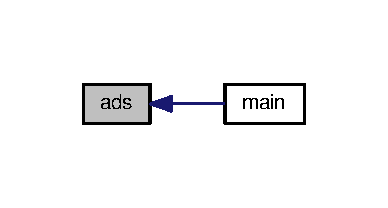
\includegraphics[width=186pt]{fluid_shader_frag_8glsl_aa92a70677efb9df36d42919ab01aaaf4_icgraph}
\end{center}
\end{figure}


\hypertarget{fluid_shader_frag_8glsl_abd810f8b2d0a0892c1c9d96228c3017d}{\index{fluid\-Shader\-Frag.\-glsl@{fluid\-Shader\-Frag.\-glsl}!uv\-To\-Eye@{uv\-To\-Eye}}
\index{uv\-To\-Eye@{uv\-To\-Eye}!fluidShaderFrag.glsl@{fluid\-Shader\-Frag.\-glsl}}
\subsubsection[{uv\-To\-Eye}]{\setlength{\rightskip}{0pt plus 5cm}vec3 uv\-To\-Eye (
\begin{DoxyParamCaption}
\item[{vec2}]{\-\_\-uv, }
\item[{float}]{\-\_\-depth}
\end{DoxyParamCaption}
)}}\label{fluid_shader_frag_8glsl_abd810f8b2d0a0892c1c9d96228c3017d}


converts uv coords and depth to eye space coodinates 


\begin{DoxyParams}{Parameters}
{\em \-\_\-uv} & -\/ texture coordinate \\
\hline
{\em \-\_\-depth} & -\/ depth at location \\
\hline
\end{DoxyParams}
\begin{DoxyReturn}{Returns}
eye space coordinate 
\end{DoxyReturn}


Here is the caller graph for this function\-:\nopagebreak
\begin{figure}[H]
\begin{center}
\leavevmode
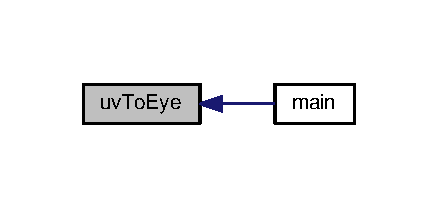
\includegraphics[width=210pt]{fluid_shader_frag_8glsl_abd810f8b2d0a0892c1c9d96228c3017d_icgraph}
\end{center}
\end{figure}



\hypertarget{fluid_shader_vert_8glsl}{\section{shaders/fluid\-Shader\-Vert.glsl File Reference}
\label{fluid_shader_vert_8glsl}\index{shaders/fluid\-Shader\-Vert.\-glsl@{shaders/fluid\-Shader\-Vert.\-glsl}}
}
\subsection*{Functions}
\begin{DoxyCompactItemize}
\item 
\hyperlink{fluid_shader_vert_8glsl_a76e82f4a2abee8cef9ec3419ca1ad185}{layout} (location=0) in vec2 vertex\-Position
\begin{DoxyCompactList}\small\item\em our vertex postion buffer \end{DoxyCompactList}\item 
\hypertarget{fluid_shader_vert_8glsl_a6288eba0f8e8ad3ab1544ad731eb7667}{void \hyperlink{fluid_shader_vert_8glsl_a6288eba0f8e8ad3ab1544ad731eb7667}{main} (void)}\label{fluid_shader_vert_8glsl_a6288eba0f8e8ad3ab1544ad731eb7667}

\begin{DoxyCompactList}\small\item\em our vertex main \end{DoxyCompactList}\end{DoxyCompactItemize}
\subsection*{Variables}
\begin{DoxyCompactItemize}
\item 
\hypertarget{fluid_shader_vert_8glsl_a849580e4568e3dc8125d8e541b50a483}{out vec2 \hyperlink{fluid_shader_vert_8glsl_a849580e4568e3dc8125d8e541b50a483}{V\-Tex\-Coord}}\label{fluid_shader_vert_8glsl_a849580e4568e3dc8125d8e541b50a483}

\begin{DoxyCompactList}\small\item\em tex\-Coords to be passed to our fragment shader \end{DoxyCompactList}\end{DoxyCompactItemize}


\subsection{Detailed Description}
\begin{DoxyAuthor}{Author}
Declan Russell 
\end{DoxyAuthor}
\begin{DoxyDate}{Date}
14/03/15 
\end{DoxyDate}
\begin{DoxyVersion}{Version}
1.\-0  G\-L\-S\-L 
\end{DoxyVersion}


\subsection{Function Documentation}
\hypertarget{fluid_shader_vert_8glsl_a76e82f4a2abee8cef9ec3419ca1ad185}{\index{fluid\-Shader\-Vert.\-glsl@{fluid\-Shader\-Vert.\-glsl}!layout@{layout}}
\index{layout@{layout}!fluidShaderVert.glsl@{fluid\-Shader\-Vert.\-glsl}}
\subsubsection[{layout}]{\setlength{\rightskip}{0pt plus 5cm}layout (
\begin{DoxyParamCaption}
\item[{location}]{ = {\ttfamily 0}}
\end{DoxyParamCaption}
)}}\label{fluid_shader_vert_8glsl_a76e82f4a2abee8cef9ec3419ca1ad185}


our vertex postion buffer 

our vertex texcoord buffer 
\hypertarget{particle_depth_frag_8glsl}{\section{/home/dexternation/\-A\-G\-S\-D\-T\-Fluid\-Sim/shaders/particle\-Depth\-Frag.glsl File Reference}
\label{particle_depth_frag_8glsl}\index{/home/dexternation/\-A\-G\-S\-D\-T\-Fluid\-Sim/shaders/particle\-Depth\-Frag.\-glsl@{/home/dexternation/\-A\-G\-S\-D\-T\-Fluid\-Sim/shaders/particle\-Depth\-Frag.\-glsl}}
}
\subsection*{Functions}
\begin{DoxyCompactItemize}
\item 
\hypertarget{particle_depth_frag_8glsl_acdef7a1fd863a6d3770c1268cb06add3}{void \hyperlink{particle_depth_frag_8glsl_acdef7a1fd863a6d3770c1268cb06add3}{main} ()}\label{particle_depth_frag_8glsl_acdef7a1fd863a6d3770c1268cb06add3}

\begin{DoxyCompactList}\small\item\em fragment main. Draws point sprites as spheres, calculates and outputs there depth. \end{DoxyCompactList}\end{DoxyCompactItemize}
\subsection*{Variables}
\begin{DoxyCompactItemize}
\item 
\hypertarget{particle_depth_frag_8glsl_a3ed508f736330bc856fb21ef562c1963}{in vec3 \hyperlink{particle_depth_frag_8glsl_a3ed508f736330bc856fb21ef562c1963}{position}}\label{particle_depth_frag_8glsl_a3ed508f736330bc856fb21ef562c1963}

\begin{DoxyCompactList}\small\item\em eye space postion from vertex shader \end{DoxyCompactList}\item 
\hypertarget{particle_depth_frag_8glsl_a59376561fcb9ace7e6531ad800fb1283}{uniform float \hyperlink{particle_depth_frag_8glsl_a59376561fcb9ace7e6531ad800fb1283}{point\-Radius}}\label{particle_depth_frag_8glsl_a59376561fcb9ace7e6531ad800fb1283}

\begin{DoxyCompactList}\small\item\em radius of our points \end{DoxyCompactList}\item 
\hypertarget{particle_depth_frag_8glsl_a06f273d5c491bfbe3897fc9c73dcf0d5}{uniform mat4 \hyperlink{particle_depth_frag_8glsl_a06f273d5c491bfbe3897fc9c73dcf0d5}{P}}\label{particle_depth_frag_8glsl_a06f273d5c491bfbe3897fc9c73dcf0d5}

\begin{DoxyCompactList}\small\item\em projection matrix \end{DoxyCompactList}\item 
\hypertarget{particle_depth_frag_8glsl_a575f888600764d6ebd67a3fd89a7d034}{out vec4 \hyperlink{particle_depth_frag_8glsl_a575f888600764d6ebd67a3fd89a7d034}{fragout}}\label{particle_depth_frag_8glsl_a575f888600764d6ebd67a3fd89a7d034}

\begin{DoxyCompactList}\small\item\em output fragment. This will be the depth of our particles \end{DoxyCompactList}\end{DoxyCompactItemize}


\subsection{Detailed Description}
\begin{DoxyAuthor}{Author}
Declan Russell 
\end{DoxyAuthor}
\begin{DoxyDate}{Date}
8/03/15 
\end{DoxyDate}
\begin{DoxyVersion}{Version}
1.\-0  G\-L\-S\-L 
\end{DoxyVersion}

\hypertarget{particle_depth_vert_8glsl}{\section{shaders/particle\-Depth\-Vert.glsl File Reference}
\label{particle_depth_vert_8glsl}\index{shaders/particle\-Depth\-Vert.\-glsl@{shaders/particle\-Depth\-Vert.\-glsl}}
}
\subsection*{Functions}
\begin{DoxyCompactItemize}
\item 
\hypertarget{particle_depth_vert_8glsl_a3a9bed495f596aa8aed4121aacc43fdd}{\hyperlink{particle_depth_vert_8glsl_a3a9bed495f596aa8aed4121aacc43fdd}{layout} (location=0) in vec3 vertex\-Position}\label{particle_depth_vert_8glsl_a3a9bed495f596aa8aed4121aacc43fdd}

\begin{DoxyCompactList}\small\item\em position of particles buffer \end{DoxyCompactList}\item 
\hypertarget{particle_depth_vert_8glsl_acdef7a1fd863a6d3770c1268cb06add3}{void \hyperlink{particle_depth_vert_8glsl_acdef7a1fd863a6d3770c1268cb06add3}{main} ()}\label{particle_depth_vert_8glsl_acdef7a1fd863a6d3770c1268cb06add3}

\begin{DoxyCompactList}\small\item\em vertex main. Scales point sprites with projection matrix and passes through eye space postion to fragment shader \end{DoxyCompactList}\end{DoxyCompactItemize}
\subsection*{Variables}
\begin{DoxyCompactItemize}
\item 
\hypertarget{particle_depth_vert_8glsl_af78042b263da1185c97c3202ced45aab}{out vec3 \hyperlink{particle_depth_vert_8glsl_af78042b263da1185c97c3202ced45aab}{position}}\label{particle_depth_vert_8glsl_af78042b263da1185c97c3202ced45aab}

\begin{DoxyCompactList}\small\item\em eye space position to be sent to fragment shader \end{DoxyCompactList}\item 
\hypertarget{particle_depth_vert_8glsl_a06f273d5c491bfbe3897fc9c73dcf0d5}{uniform mat4 \hyperlink{particle_depth_vert_8glsl_a06f273d5c491bfbe3897fc9c73dcf0d5}{P}}\label{particle_depth_vert_8glsl_a06f273d5c491bfbe3897fc9c73dcf0d5}

\begin{DoxyCompactList}\small\item\em our projection matrix \end{DoxyCompactList}\item 
\hypertarget{particle_depth_vert_8glsl_aea165d91373502f69ddf839215635405}{uniform mat4 \hyperlink{particle_depth_vert_8glsl_aea165d91373502f69ddf839215635405}{M\-V}}\label{particle_depth_vert_8glsl_aea165d91373502f69ddf839215635405}

\begin{DoxyCompactList}\small\item\em our model view matrix \end{DoxyCompactList}\item 
\hypertarget{particle_depth_vert_8glsl_ae56d8b04842b99426c8844c0785d3090}{uniform mat4 \hyperlink{particle_depth_vert_8glsl_ae56d8b04842b99426c8844c0785d3090}{M\-V\-P}}\label{particle_depth_vert_8glsl_ae56d8b04842b99426c8844c0785d3090}

\begin{DoxyCompactList}\small\item\em our model view projection matrix \end{DoxyCompactList}\item 
\hypertarget{particle_depth_vert_8glsl_a62a808a061d03e4a62f2d46d3e6efb38}{uniform int \hyperlink{particle_depth_vert_8glsl_a62a808a061d03e4a62f2d46d3e6efb38}{screen\-Width}}\label{particle_depth_vert_8glsl_a62a808a061d03e4a62f2d46d3e6efb38}

\begin{DoxyCompactList}\small\item\em the width of our screen \end{DoxyCompactList}\item 
\hypertarget{particle_depth_vert_8glsl_a9550a4bf60e3039a98ab946ba37ae067}{uniform float \hyperlink{particle_depth_vert_8glsl_a9550a4bf60e3039a98ab946ba37ae067}{point\-Size}}\label{particle_depth_vert_8glsl_a9550a4bf60e3039a98ab946ba37ae067}

\begin{DoxyCompactList}\small\item\em the size of our particles \end{DoxyCompactList}\end{DoxyCompactItemize}


\subsection{Detailed Description}
\begin{DoxyAuthor}{Author}
Declan Russell 
\end{DoxyAuthor}
\begin{DoxyDate}{Date}
8/03/15 
\end{DoxyDate}
\begin{DoxyVersion}{Version}
1.\-0  G\-L\-S\-L 
\end{DoxyVersion}

\hypertarget{sky_box_frag_8glsl}{\section{shaders/sky\-Box\-Frag.glsl File Reference}
\label{sky_box_frag_8glsl}\index{shaders/sky\-Box\-Frag.\-glsl@{shaders/sky\-Box\-Frag.\-glsl}}
}
\subsection*{Functions}
\begin{DoxyCompactItemize}
\item 
\hypertarget{sky_box_frag_8glsl_acdef7a1fd863a6d3770c1268cb06add3}{void \hyperlink{sky_box_frag_8glsl_acdef7a1fd863a6d3770c1268cb06add3}{main} ()}\label{sky_box_frag_8glsl_acdef7a1fd863a6d3770c1268cb06add3}

\begin{DoxyCompactList}\small\item\em fragment main for shading our cubemap. \end{DoxyCompactList}\end{DoxyCompactItemize}
\subsection*{Variables}
\begin{DoxyCompactItemize}
\item 
\hypertarget{sky_box_frag_8glsl_a4989ba8cb91a639702eb2204f23cf73f}{in vec3 \hyperlink{sky_box_frag_8glsl_a4989ba8cb91a639702eb2204f23cf73f}{texcoords}}\label{sky_box_frag_8glsl_a4989ba8cb91a639702eb2204f23cf73f}

\begin{DoxyCompactList}\small\item\em texture coordinates of our cube from vertex shader \end{DoxyCompactList}\item 
\hypertarget{sky_box_frag_8glsl_a9dac566b8dcb58f380dec54a9a51b3fa}{uniform sampler\-Cube \hyperlink{sky_box_frag_8glsl_a9dac566b8dcb58f380dec54a9a51b3fa}{cube\-Map\-Tex}}\label{sky_box_frag_8glsl_a9dac566b8dcb58f380dec54a9a51b3fa}

\begin{DoxyCompactList}\small\item\em cube map sampler \end{DoxyCompactList}\item 
\hypertarget{sky_box_frag_8glsl_ae6bde93c13ab90b831d2986a7de2d347}{out vec4 \hyperlink{sky_box_frag_8glsl_ae6bde93c13ab90b831d2986a7de2d347}{fragcolour}}\label{sky_box_frag_8glsl_ae6bde93c13ab90b831d2986a7de2d347}

\begin{DoxyCompactList}\small\item\em our output fragment \end{DoxyCompactList}\end{DoxyCompactItemize}


\subsection{Detailed Description}
\begin{DoxyAuthor}{Author}
Declan Russell 
\end{DoxyAuthor}
\begin{DoxyDate}{Date}
15/03/15 
\end{DoxyDate}
\begin{DoxyVersion}{Version}
1.\-0  G\-L\-S\-L 
\end{DoxyVersion}

\hypertarget{sky_box_vert_8glsl}{\section{shaders/sky\-Box\-Vert.glsl File Reference}
\label{sky_box_vert_8glsl}\index{shaders/sky\-Box\-Vert.\-glsl@{shaders/sky\-Box\-Vert.\-glsl}}
}
\subsection*{Functions}
\begin{DoxyCompactItemize}
\item 
\hypertarget{sky_box_vert_8glsl_a3a9bed495f596aa8aed4121aacc43fdd}{\hyperlink{sky_box_vert_8glsl_a3a9bed495f596aa8aed4121aacc43fdd}{layout} (location=0) in vec3 vertex\-Position}\label{sky_box_vert_8glsl_a3a9bed495f596aa8aed4121aacc43fdd}

\begin{DoxyCompactList}\small\item\em vertex position buffer \end{DoxyCompactList}\item 
\hypertarget{sky_box_vert_8glsl_acdef7a1fd863a6d3770c1268cb06add3}{void \hyperlink{sky_box_vert_8glsl_acdef7a1fd863a6d3770c1268cb06add3}{main} ()}\label{sky_box_vert_8glsl_acdef7a1fd863a6d3770c1268cb06add3}

\begin{DoxyCompactList}\small\item\em vertex shader main. Just passes texcoords and M\-V\-P$\ast$vertex\-Positons \end{DoxyCompactList}\end{DoxyCompactItemize}
\subsection*{Variables}
\begin{DoxyCompactItemize}
\item 
\hypertarget{sky_box_vert_8glsl_ae56d8b04842b99426c8844c0785d3090}{uniform mat4 \hyperlink{sky_box_vert_8glsl_ae56d8b04842b99426c8844c0785d3090}{M\-V\-P}}\label{sky_box_vert_8glsl_ae56d8b04842b99426c8844c0785d3090}

\begin{DoxyCompactList}\small\item\em Model view projection matrix uniform. \end{DoxyCompactList}\item 
\hypertarget{sky_box_vert_8glsl_a71c0fbb5bdc732da08d0a88822242470}{out vec3 \hyperlink{sky_box_vert_8glsl_a71c0fbb5bdc732da08d0a88822242470}{texcoords}}\label{sky_box_vert_8glsl_a71c0fbb5bdc732da08d0a88822242470}

\begin{DoxyCompactList}\small\item\em texture coords to be passed to our fragment shader \end{DoxyCompactList}\end{DoxyCompactItemize}


\subsection{Detailed Description}
\begin{DoxyAuthor}{Author}
Declan Russell 
\end{DoxyAuthor}
\begin{DoxyDate}{Date}
15/03/15 
\end{DoxyDate}
\begin{DoxyVersion}{Version}
1.\-0  G\-L\-S\-L 
\end{DoxyVersion}

\hypertarget{thickness_frag_8glsl}{\section{shaders/thickness\-Frag.glsl File Reference}
\label{thickness_frag_8glsl}\index{shaders/thickness\-Frag.\-glsl@{shaders/thickness\-Frag.\-glsl}}
}
\subsection*{Functions}
\begin{DoxyCompactItemize}
\item 
\hypertarget{thickness_frag_8glsl_acdef7a1fd863a6d3770c1268cb06add3}{void \hyperlink{thickness_frag_8glsl_acdef7a1fd863a6d3770c1268cb06add3}{main} ()}\label{thickness_frag_8glsl_acdef7a1fd863a6d3770c1268cb06add3}

\begin{DoxyCompactList}\small\item\em fragment main. Draws spheres from point sprites colored by our thickness scaler \end{DoxyCompactList}\end{DoxyCompactItemize}
\subsection*{Variables}
\begin{DoxyCompactItemize}
\item 
\hypertarget{thickness_frag_8glsl_a3ed508f736330bc856fb21ef562c1963}{in vec3 \hyperlink{thickness_frag_8glsl_a3ed508f736330bc856fb21ef562c1963}{position}}\label{thickness_frag_8glsl_a3ed508f736330bc856fb21ef562c1963}

\begin{DoxyCompactList}\small\item\em eye space postion from vertex shader \end{DoxyCompactList}\item 
\hypertarget{thickness_frag_8glsl_a59376561fcb9ace7e6531ad800fb1283}{uniform float \hyperlink{thickness_frag_8glsl_a59376561fcb9ace7e6531ad800fb1283}{point\-Radius}}\label{thickness_frag_8glsl_a59376561fcb9ace7e6531ad800fb1283}

\begin{DoxyCompactList}\small\item\em radius of our points \end{DoxyCompactList}\item 
\hypertarget{thickness_frag_8glsl_a18b0d87ec9f888da1e3236e988aaebaf}{uniform float \hyperlink{thickness_frag_8glsl_a18b0d87ec9f888da1e3236e988aaebaf}{thickness\-Scaler}}\label{thickness_frag_8glsl_a18b0d87ec9f888da1e3236e988aaebaf}

\begin{DoxyCompactList}\small\item\em scaler for our thickness \end{DoxyCompactList}\item 
\hypertarget{thickness_frag_8glsl_a575f888600764d6ebd67a3fd89a7d034}{out vec4 \hyperlink{thickness_frag_8glsl_a575f888600764d6ebd67a3fd89a7d034}{fragout}}\label{thickness_frag_8glsl_a575f888600764d6ebd67a3fd89a7d034}

\begin{DoxyCompactList}\small\item\em the output fragment \end{DoxyCompactList}\end{DoxyCompactItemize}


\subsection{Detailed Description}
\begin{DoxyAuthor}{Author}
Declan Russell 
\end{DoxyAuthor}
\begin{DoxyDate}{Date}
15/03/15 
\end{DoxyDate}
\begin{DoxyVersion}{Version}
1.\-0  G\-L\-S\-L 
\end{DoxyVersion}

\hypertarget{thickness_vert_8glsl}{\section{shaders/thickness\-Vert.glsl File Reference}
\label{thickness_vert_8glsl}\index{shaders/thickness\-Vert.\-glsl@{shaders/thickness\-Vert.\-glsl}}
}
\subsection*{Functions}
\begin{DoxyCompactItemize}
\item 
\hypertarget{thickness_vert_8glsl_a3a9bed495f596aa8aed4121aacc43fdd}{\hyperlink{thickness_vert_8glsl_a3a9bed495f596aa8aed4121aacc43fdd}{layout} (location=0) in vec3 vertex\-Position}\label{thickness_vert_8glsl_a3a9bed495f596aa8aed4121aacc43fdd}

\begin{DoxyCompactList}\small\item\em position of particles buffer \end{DoxyCompactList}\item 
\hypertarget{thickness_vert_8glsl_acdef7a1fd863a6d3770c1268cb06add3}{void \hyperlink{thickness_vert_8glsl_acdef7a1fd863a6d3770c1268cb06add3}{main} ()}\label{thickness_vert_8glsl_acdef7a1fd863a6d3770c1268cb06add3}

\begin{DoxyCompactList}\small\item\em vertex main. Scales point sprites with projection matrix and passes through eye space postion to fragment shader \end{DoxyCompactList}\end{DoxyCompactItemize}
\subsection*{Variables}
\begin{DoxyCompactItemize}
\item 
\hypertarget{thickness_vert_8glsl_af78042b263da1185c97c3202ced45aab}{out vec3 \hyperlink{thickness_vert_8glsl_af78042b263da1185c97c3202ced45aab}{position}}\label{thickness_vert_8glsl_af78042b263da1185c97c3202ced45aab}

\begin{DoxyCompactList}\small\item\em eye space position to be sent to fragment shader \end{DoxyCompactList}\item 
\hypertarget{thickness_vert_8glsl_a06f273d5c491bfbe3897fc9c73dcf0d5}{uniform mat4 \hyperlink{thickness_vert_8glsl_a06f273d5c491bfbe3897fc9c73dcf0d5}{P}}\label{thickness_vert_8glsl_a06f273d5c491bfbe3897fc9c73dcf0d5}

\begin{DoxyCompactList}\small\item\em our projection matrix \end{DoxyCompactList}\item 
\hypertarget{thickness_vert_8glsl_aea165d91373502f69ddf839215635405}{uniform mat4 \hyperlink{thickness_vert_8glsl_aea165d91373502f69ddf839215635405}{M\-V}}\label{thickness_vert_8glsl_aea165d91373502f69ddf839215635405}

\begin{DoxyCompactList}\small\item\em our model view matrix \end{DoxyCompactList}\item 
\hypertarget{thickness_vert_8glsl_ae56d8b04842b99426c8844c0785d3090}{uniform mat4 \hyperlink{thickness_vert_8glsl_ae56d8b04842b99426c8844c0785d3090}{M\-V\-P}}\label{thickness_vert_8glsl_ae56d8b04842b99426c8844c0785d3090}

\begin{DoxyCompactList}\small\item\em our model view projection matrix \end{DoxyCompactList}\item 
\hypertarget{thickness_vert_8glsl_a62a808a061d03e4a62f2d46d3e6efb38}{uniform int \hyperlink{thickness_vert_8glsl_a62a808a061d03e4a62f2d46d3e6efb38}{screen\-Width}}\label{thickness_vert_8glsl_a62a808a061d03e4a62f2d46d3e6efb38}

\begin{DoxyCompactList}\small\item\em the width of our screen \end{DoxyCompactList}\item 
\hypertarget{thickness_vert_8glsl_a9550a4bf60e3039a98ab946ba37ae067}{uniform float \hyperlink{thickness_vert_8glsl_a9550a4bf60e3039a98ab946ba37ae067}{point\-Size}}\label{thickness_vert_8glsl_a9550a4bf60e3039a98ab946ba37ae067}

\begin{DoxyCompactList}\small\item\em the size of our particles \end{DoxyCompactList}\end{DoxyCompactItemize}


\subsection{Detailed Description}
\begin{DoxyAuthor}{Author}
Declan Russell 
\end{DoxyAuthor}
\begin{DoxyDate}{Date}
15/03/15 
\end{DoxyDate}
\begin{DoxyVersion}{Version}
1.\-0  G\-L\-S\-L 
\end{DoxyVersion}

%--- End generated contents ---

% Index
\newpage
\phantomsection
\addcontentsline{toc}{chapter}{Index}
\printindex

\end{document}
